% Options for packages loaded elsewhere
\PassOptionsToPackage{unicode}{hyperref}
\PassOptionsToPackage{hyphens}{url}
%
\documentclass[
]{book}
\usepackage{lmodern}
\usepackage{amssymb,amsmath}
\usepackage{ifxetex,ifluatex}
\ifnum 0\ifxetex 1\fi\ifluatex 1\fi=0 % if pdftex
  \usepackage[T1]{fontenc}
  \usepackage[utf8]{inputenc}
  \usepackage{textcomp} % provide euro and other symbols
\else % if luatex or xetex
  \usepackage{unicode-math}
  \defaultfontfeatures{Scale=MatchLowercase}
  \defaultfontfeatures[\rmfamily]{Ligatures=TeX,Scale=1}
\fi
% Use upquote if available, for straight quotes in verbatim environments
\IfFileExists{upquote.sty}{\usepackage{upquote}}{}
\IfFileExists{microtype.sty}{% use microtype if available
  \usepackage[]{microtype}
  \UseMicrotypeSet[protrusion]{basicmath} % disable protrusion for tt fonts
}{}
\makeatletter
\@ifundefined{KOMAClassName}{% if non-KOMA class
  \IfFileExists{parskip.sty}{%
    \usepackage{parskip}
  }{% else
    \setlength{\parindent}{0pt}
    \setlength{\parskip}{6pt plus 2pt minus 1pt}}
}{% if KOMA class
  \KOMAoptions{parskip=half}}
\makeatother
\usepackage{xcolor}
\IfFileExists{xurl.sty}{\usepackage{xurl}}{} % add URL line breaks if available
\IfFileExists{bookmark.sty}{\usepackage{bookmark}}{\usepackage{hyperref}}
\hypersetup{
  pdftitle={Audit Analytics with R},
  pdfauthor={Jonathan Lin},
  hidelinks,
  pdfcreator={LaTeX via pandoc}}
\urlstyle{same} % disable monospaced font for URLs
\usepackage{color}
\usepackage{fancyvrb}
\newcommand{\VerbBar}{|}
\newcommand{\VERB}{\Verb[commandchars=\\\{\}]}
\DefineVerbatimEnvironment{Highlighting}{Verbatim}{commandchars=\\\{\}}
% Add ',fontsize=\small' for more characters per line
\usepackage{framed}
\definecolor{shadecolor}{RGB}{248,248,248}
\newenvironment{Shaded}{\begin{snugshade}}{\end{snugshade}}
\newcommand{\AlertTok}[1]{\textcolor[rgb]{0.94,0.16,0.16}{#1}}
\newcommand{\AnnotationTok}[1]{\textcolor[rgb]{0.56,0.35,0.01}{\textbf{\textit{#1}}}}
\newcommand{\AttributeTok}[1]{\textcolor[rgb]{0.77,0.63,0.00}{#1}}
\newcommand{\BaseNTok}[1]{\textcolor[rgb]{0.00,0.00,0.81}{#1}}
\newcommand{\BuiltInTok}[1]{#1}
\newcommand{\CharTok}[1]{\textcolor[rgb]{0.31,0.60,0.02}{#1}}
\newcommand{\CommentTok}[1]{\textcolor[rgb]{0.56,0.35,0.01}{\textit{#1}}}
\newcommand{\CommentVarTok}[1]{\textcolor[rgb]{0.56,0.35,0.01}{\textbf{\textit{#1}}}}
\newcommand{\ConstantTok}[1]{\textcolor[rgb]{0.00,0.00,0.00}{#1}}
\newcommand{\ControlFlowTok}[1]{\textcolor[rgb]{0.13,0.29,0.53}{\textbf{#1}}}
\newcommand{\DataTypeTok}[1]{\textcolor[rgb]{0.13,0.29,0.53}{#1}}
\newcommand{\DecValTok}[1]{\textcolor[rgb]{0.00,0.00,0.81}{#1}}
\newcommand{\DocumentationTok}[1]{\textcolor[rgb]{0.56,0.35,0.01}{\textbf{\textit{#1}}}}
\newcommand{\ErrorTok}[1]{\textcolor[rgb]{0.64,0.00,0.00}{\textbf{#1}}}
\newcommand{\ExtensionTok}[1]{#1}
\newcommand{\FloatTok}[1]{\textcolor[rgb]{0.00,0.00,0.81}{#1}}
\newcommand{\FunctionTok}[1]{\textcolor[rgb]{0.00,0.00,0.00}{#1}}
\newcommand{\ImportTok}[1]{#1}
\newcommand{\InformationTok}[1]{\textcolor[rgb]{0.56,0.35,0.01}{\textbf{\textit{#1}}}}
\newcommand{\KeywordTok}[1]{\textcolor[rgb]{0.13,0.29,0.53}{\textbf{#1}}}
\newcommand{\NormalTok}[1]{#1}
\newcommand{\OperatorTok}[1]{\textcolor[rgb]{0.81,0.36,0.00}{\textbf{#1}}}
\newcommand{\OtherTok}[1]{\textcolor[rgb]{0.56,0.35,0.01}{#1}}
\newcommand{\PreprocessorTok}[1]{\textcolor[rgb]{0.56,0.35,0.01}{\textit{#1}}}
\newcommand{\RegionMarkerTok}[1]{#1}
\newcommand{\SpecialCharTok}[1]{\textcolor[rgb]{0.00,0.00,0.00}{#1}}
\newcommand{\SpecialStringTok}[1]{\textcolor[rgb]{0.31,0.60,0.02}{#1}}
\newcommand{\StringTok}[1]{\textcolor[rgb]{0.31,0.60,0.02}{#1}}
\newcommand{\VariableTok}[1]{\textcolor[rgb]{0.00,0.00,0.00}{#1}}
\newcommand{\VerbatimStringTok}[1]{\textcolor[rgb]{0.31,0.60,0.02}{#1}}
\newcommand{\WarningTok}[1]{\textcolor[rgb]{0.56,0.35,0.01}{\textbf{\textit{#1}}}}
\usepackage{longtable,booktabs}
% Correct order of tables after \paragraph or \subparagraph
\usepackage{etoolbox}
\makeatletter
\patchcmd\longtable{\par}{\if@noskipsec\mbox{}\fi\par}{}{}
\makeatother
% Allow footnotes in longtable head/foot
\IfFileExists{footnotehyper.sty}{\usepackage{footnotehyper}}{\usepackage{footnote}}
\makesavenoteenv{longtable}
\usepackage{graphicx,grffile}
\makeatletter
\def\maxwidth{\ifdim\Gin@nat@width>\linewidth\linewidth\else\Gin@nat@width\fi}
\def\maxheight{\ifdim\Gin@nat@height>\textheight\textheight\else\Gin@nat@height\fi}
\makeatother
% Scale images if necessary, so that they will not overflow the page
% margins by default, and it is still possible to overwrite the defaults
% using explicit options in \includegraphics[width, height, ...]{}
\setkeys{Gin}{width=\maxwidth,height=\maxheight,keepaspectratio}
% Set default figure placement to htbp
\makeatletter
\def\fps@figure{htbp}
\makeatother
\usepackage[normalem]{ulem}
% Avoid problems with \sout in headers with hyperref
\pdfstringdefDisableCommands{\renewcommand{\sout}{}}
\setlength{\emergencystretch}{3em} % prevent overfull lines
\providecommand{\tightlist}{%
  \setlength{\itemsep}{0pt}\setlength{\parskip}{0pt}}
\setcounter{secnumdepth}{5}
\usepackage{amsmath}
\usepackage{booktabs}
\usepackage{caption}
\usepackage{longtable}

\title{Audit Analytics with R}
\author{Jonathan Lin}
\date{2020-10-29}

\begin{document}
\maketitle

{
\setcounter{tocdepth}{1}
\tableofcontents
}
\hypertarget{welcome}{%
\chapter*{Welcome}\label{welcome}}
\addcontentsline{toc}{chapter}{Welcome}

\emph{Draft Version - Please post any \href{https://github.com/jonlinca/auditanalytics/issues}{issues} found}

This is the website for Audit Analytics in R. This audience of this book is for:

\begin{itemize}
\tightlist
\item
  Audit leaders who are looking to design their environment to encourage cultivate collaboration and sustainability.
\item
  Audit data analytics practitioners, who are looking to leverage R in their data analytics tasks.
\end{itemize}

You will learn what tools and technologies are well suited for a modern audit analytics toolkit, as well as learn skills with R to perform data analytics tasks. Consider this book to be your roadmap of practical items to implement and follow.

If you are brand new to R, I encourage you to read \url{https://rstudio-education.github.io/hopr/} and \url{https://r4ds.had.co.nz}. While some limited foundations and explanations will be provided, this book is focused on an applied view of R to the financial auditor practice.

\hypertarget{about-the-author}{%
\chapter*{About the author}\label{about-the-author}}
\addcontentsline{toc}{chapter}{About the author}

\hypertarget{intro}{%
\chapter{Introduction}\label{intro}}

Within the accounting and audit profession, analytics has been around for several decades, under the concept of Computer Aided Auditing Techniques (CAATs). The software of choice was led by ACL and its ACL Analytics software. ACL Analytics was a significant audit enabler at the time, as it allowed direct access to analyze mainframe data and flat files that were otherwise inaccessible by mainstream software on the market. It enabled audit teams to obtain transparency in analysis, a rigorous audit trail, and even automation of scripts.

As computers, data analytic technology and accessibility of coding in the Accounting practice has become mainstream, there are far more tools that enable auditors to become far more powerful and self sufficient than ever before. Tools that are typically reserved for software engineers and statisticians have empowered financial auditors to expand their breadth and scope.

A traditional internal audit team would consider themselves to be consumers of information, limited by flat files sent by emails from their stakeholders. While most internal auditors have implemented data analytics in one way or another, the realm of possibilities and challenges have outpaced audit shop capabilities. The expectation now is for auditors to be fully integrated into the business, and contribute directly to the management of the financial and IT risks the company faces on a regular basis.

The most effective way to meet this new standard is to implement a current data analytics architecture and empower your team to leverage modern data analytics techniques.

\hypertarget{part-structure}{%
\part{Structure}\label{part-structure}}

\hypertarget{approach}{%
\chapter{Approach}\label{approach}}

For many audit teams, having data analytics employed in your audit team is generally a given. The advantages are well articulated - 100\% population coverage, timely response, and targeted high risk identification and results are true and real.

Unfortunately, any short-burst of investment in data analytics training tends to not last more than a few months. This is due to lack of applied skills, sustained management interest, and consistency of values. While regulations for adherence to SEC and Sox requirements exist and are necessary, the means to approaching and achieving compliance has been largely static in nature since the introduction of Sox.

The root cause is that audit teams culturally view analytics as a skill, and not as a cultural shift. On a micro level, while not every individual on your audit team needs to be a `coder', everyone needs to share the same values and philosophy for any audit analytics program to have success. Your core analytics team will set the foundation for the rest of the team to play on - if the non-data members don't show up, the analytics program is limited at best.

Having a combination of the right values and technologies will enable your team to propel forward, and should amplify your teams efforts. By thoughtfully choosing your tools and encouraging sustainable processes, your team will create a positive cycle of development, learning and deployment.

\hypertarget{code-based-development}{%
\section{Code-based development}\label{code-based-development}}

Consider the creation and auditing of a spreadsheet, where every row and column has the potential to be manipulated. Following the motto, `trust but verify', an auditor would need to examine each cell value, the formulas, the relationships, and keep a sharp eye out for manual adjustments. The auditor also needs to validate the source of data in the spreadsheet. With no built-in traceability to how the spreadsheet is used after it has been created, it contributes to the madness that is the spreadsheet ecosystem.

While it is easier to superficially consume information from a spreadsheet, to understand the inner workings is a tedious task into itself. And unfortunately, both controls and audits are conducted without a second thought within spreadsheets, as it is easier to tackle the task without fundamentally changing the approach itself.

Contrast this to a code-based environment. To achieve anything in code, you need to be explicit and specific on the mechanisms taken to reach the end state. Each line will tell the program what inputs it needs, how it is processed, and the collection of lines tells you what is achieved. The beauty of this is that it also tells the reader exactly what was executed to achieve the end result. A code based environment is inherently self documenting.

Once a baseline code has been established, finding ongoing changes becomes trivial. Similar to Track Changes or blackline comparisons in Microsoft Word or Google Docs, its far easier to detect how code (and the process it supports) has changed.

Perhaps with some merit, code can be difficult to read at times, as it is still a completely different language. \textbf{Notebooks} address this problem. Notebooks are interactive renderings of code, containing not only the code, but can also include sections of commentary as to why something was done, and can include data visualizations and interactivity. It is the ultimate form of auditability.

\hypertarget{automate-relentlessly}{%
\section{Automate relentlessly}\label{automate-relentlessly}}

By writing your routines in code, then the next logical step is to automate. Automation not only frees up your time from performing a task, but it also frees up your mental critical thinking and creative processing power. Every professional has a cognitive load - don't waste it on routine tasks.

A common use case for automation in audit is the creation of a \textbf{data mart} that is relevant to auditors. A data mart is a collection of pre-processed data that is suited for the group using it - for example, a data mart may hold a daily refresh of HR information, or the prior month's vendor invoices. Imagine that instead of needing to email HR for the latest employee list, the audit team merely needs to check within its internal database, making research and response quick and efficient. Instead of asking the vendor management team on how much money was spent per vendor, having this information in an audit mart readily available means you can spend more time thinking about how to assess these vendors for risk.

Gone are the days where you only audit a topic once a year. A byproduct of every audit is a monitoring mechanism - how do you know something has gone off the rails? Traditional remediation paths include a follow-up in the future - after that, there are few mechanisms to faithfully maintain confidence that the process is still operating reasonably.

If you've coded your audit, then you have already done the hard work of structuring how to extract your data, finding exceptions and distributing actionable results for your stakeholders. Automation takes that one step further, and allows you to ensure the steps are done repeatedly. The value you derived initially from your audit can now be done continuously.

Once you've audited the identification of issues and the metrics around them, then you can focus on the automation of work flow and resolution of them. With an audit controls database, you can upload the results of controls testing and issues identification into it, which will enable on-demand availability, visibility, transparency, and even reporting, all which can now be part of that larger automation process.

\hypertarget{share-everything}{%
\section{Share everything}\label{share-everything}}

\begin{quote}
Tribal knowledge is information or knowledge that is known within a tribe but often unknown outside of it. A tribe, in this sense, may be a group or subgroup of people that share such a common knowledge. From a corporate perspective, ``Tribal Knowledge or know-how is the collective wisdom of the organization. It is the sum of all the knowledge and capabilities of all the people''. (``Tribal Knowledge'' \protect\hyperlink{ref-tribal-knowledge}{2020})
\end{quote}

When you code the procedures, not only are you creating letters to yourself in the future, but you're also writing letters to everyone else on your team, even those who haven't joined. These fully contained notebooks serve as a guide to those on your team who are learning what you have developed.

The next thing to do is to put them in a central location where everyone on your team can access them. While you can opt for files and folders on a network drive, more practical technologies exist. \textbf{Code repositories}, such as the technology `git', serve a purpose in your data analytics environment to track changes to code and notebooks. You can encourage your team to upload notebooks to these repositories to access the latest and greatest code that your team has developed for problems already solved. New team members can go into a repository to learn how code has solved prior problems, and become inspired to solve problems of their own.

As your team gains more experience and consistency, it may be more practical to write repeatable processes and functions instead of copy and pasting code between notebooks. Code \textbf{packages} enable you to share your code and functions to solve specific problems, templates to encourage consistency amongst team members, and are easily distributed to your team for quick deployment.

\hypertarget{always-deliver-useful-product}{%
\section{Always deliver useful product}\label{always-deliver-useful-product}}

The outputs of your work are useless if they are not adopted by the business. This means you need to prioritize your customer and iterate often, to win buy-in, gain momentum and stay on course.

Audit teams are always surprised when I say that they have customers. Audit department interactions are across the entire company and up-and-down the entire chain - from manufacturing to engineering, IT to accounting, analysts to the c-suite. Audit departments handle all these groups, with kid-gloves and diplomacy. Yet we tend to ignore the \#1 customer - ourselves. Audit teams are usually at the mercy of what the business deems most convenient for them - whether in terms of reports, testing controls or even where files are kept.

Historically, this was tolerated. Audit teams were composed of accountants that specialized in Excel, IT auditors in testing general controls, and a focus adhering to evolving accounting standards. With the advance in maturity of code-based tools and even commercial audit software, there has never been a better time to code intuition.

The idea of these data products is that they promote the cognitive ease - this means, repeated experience, clear display, primed idea, and good mood.(Kahneman \protect\hyperlink{ref-cognitive-ease}{2011}) By helping your team feel at ease, but they should deliver both the most trivial of tasks and the most time-consuming tests of applied knowledge. By removing the need to execute these tasks, then the customer can focus on what they're good at - in the case of auditors, its applying professional judgement. These products can be taken up in the form of data generation, data and trend visualization, or standardized reporting.

\hypertarget{dont-be-a-hero}{%
\section{Don't be a hero}\label{dont-be-a-hero}}

Not everything needs to be fixed by you, especially in code. In a well-functioning organization where hundreds of people are supporting different software, application or databases, sometimes the best way to solve the problems found isn't directly in the work you do, but how you get others to fix systemic issues in the source itself. Key indicators of this are when you have to start hard-coding compensating controls in your code because the upstream data isn't standardized.

For example, in a typical company, employees are issued unique ID numbers. This is preferably at the source of truth - the Human Resources department. This identifier is generally considered reliable and stable, especially if is the source of truth. Consider now that you're now trying to join the data to a credit card system, where employees are issued credit cards based on their first and last name. If you take an assumption to join this dataset using an individuals first and last name, that would be a reasonable first attempt. However, last names can change over time, or individuals may prefer to go with their middle names, or even simple spelling mistakes can occur. Instead of compensating by adding different ways of `joining' information, its more effective to work with the application's data owner to see if they would be willing to adopt the unique employee ID instead as a field in their system.

\hypertarget{the-opportunity-cost}{%
\section{``The opportunity cost''}\label{the-opportunity-cost}}

\begin{quote}
The idea of opportunity costs presumes the fungibility of human experience: all our activities are equivalent or interchangeable once they are reduced to the abstract currency of clock time, and its wage correlate. (Crawford \protect\hyperlink{ref-shop-class}{2009})
\end{quote}

An internal auditors' largest limitation is time. The biggest barrier to the adoption and execution of data analytic talents is the fact there is `more' perceived value in doing something else. A common excuse is that a task will only be performed once (or even worse, at an irregular basis) - auditors may instead opt to perform a manual task in an unsustainable way. Instead of learning a new skill, our opportunity cost is projected against how much time can be used have to perform this task at hand.

If your existence was highly limited by the lifespan of a fly, it would be hard to argue against such a position. However, your career is long (hopefully), fruitful and full of exciting and interesting work.

Truly engaging work should challenging and rewarding, and applying coding to audit lends itself to a skill worth mastering. Using these skills, no matter how immature, will continue to pay off dividends in future implementations, no matter how insignificant or incremental. Implementing repeatable processes means not only does the end consumer receive their product quicker, but the data auditor is enabled to continuously refine or tackle another code-related problem. And that is worth the opportunity cost, today.

\hypertarget{architecture}{%
\chapter{Architecture}\label{architecture}}

\begin{figure}

{\centering 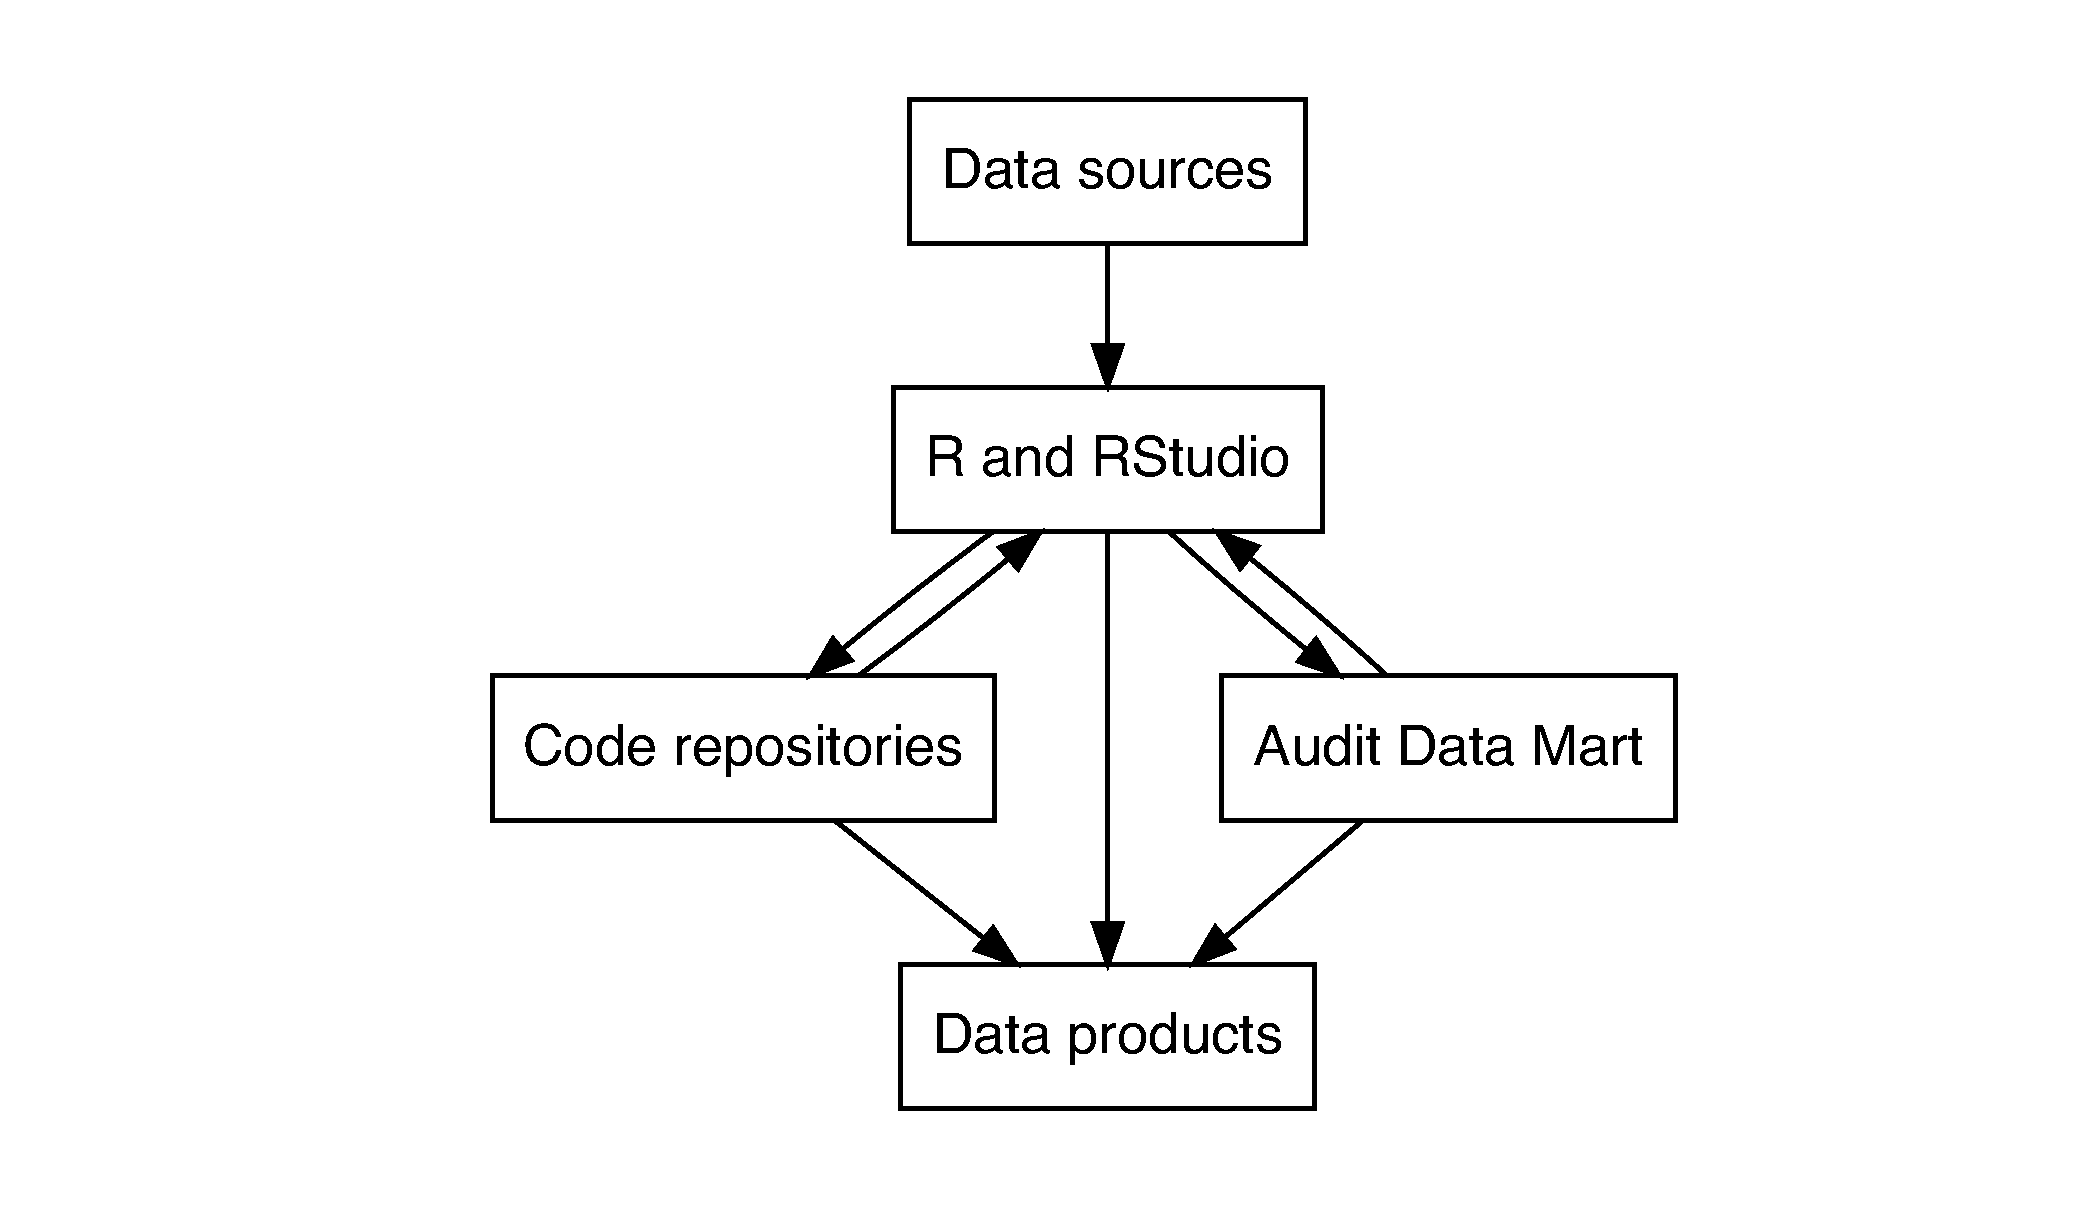
\includegraphics[width=1\linewidth]{Audit_Analytics_with-R_files/figure-latex/architecture-1} 

}

\caption{Internal Audit Data Analytics Architecture}\label{fig:architecture}
\end{figure}

The architecture and tools you select should support and amplify your team, and not be a burden to maintain. Maintenance of databases and applications can also be delegated to application support teams, so you can focus on implementing analytics and delivering data products.

Other things to consider: You should have, at a bare minimum, direct access to read-only internal databases or data warehouses. A generic service user account has its merits here when it comes to automation - tying an eventual automation to a user with password expiry every 90 days will make updating passwords feel like quarterly financial reporting.

Any software you consider should be able to talk to your company's internal and external applications. Be wary of software that locks you in or makes access to data cumbersome, as it limits your ability to integrate with your company's tools as you gain sophistication.

\hypertarget{architecture-r}{%
\section{R and RStudio}\label{architecture-r}}

\href{https://www.r-project.org}{R} is a programming language with an emphasis on statistics. It is considered free software, free in the perspective that you can run, distribute, and change it as you like.

What makes R so great is the large suite of packages that are available to use to help analyze information. This is distributed through \href{https://cran.r-project.org}{CRAN}, which is the central repository for R packages that meet minimum quality standards. What doesn't exist in base R will likely have been developed by someone else: there are hundreds of packages that support data connectivity (\href{https://cran.r-project.org/web/packages/DBI/}{DBI}, \href{https://cran.r-project.org/web/packages/xlsx/}{xlsx}), day-to-day manipulation and analysis (\href{https://cran.r-project.org/web/packages/dplyr/}{dplyr}, \href{https://cran.r-project.org/web/packages/ggplot2/}{ggplot2}), and even auditing (\href{https://cran.r-project.org/web/packages/jfa/}{jfa}, \href{https://cran.r-project.org/web/packages/MUS/}{MUS}).

As R is a language, you may want to consider an application to code in, similar to how you may write memos in Microsoft Word. \href{https://rstudio.com}{RStudio Desktop} is an integrated development environment (IDE) that has an open source version and is free to use. There are also free versions of RStudio Server, as well as commercially supported versions of its Desktop, Server, and two unique products that we will go into more later - Package Manager and Connect.

With both R and RStudio installed, you can perform the minimum requirements of your audit data analysis career: you can download data, wrangle it, visualize it, and save completed analyses. The potential is limitless though, as it enables all the other technologies to operate with it - machine learning, automation, dashboarding, and code sharing.

\hypertarget{code-repositories}{%
\section{Code repositories}\label{code-repositories}}

Here is a typical logistical challenge faced in even the smallest of audit teams. Person A will write the first version of a script to download data (version 1). Person B in the team may want to use it to download data from elsewhere, so they will get an emailed script file from person B, modify it, and start to use it. Person A may make improvements to their own file (now version 2), but Person B will not benefit from the improvements. Knowledge are immediately siloed, and changes become more difficult to share between auditors.

One of the most effective ways to solve this problem is to leverage a code repository (also known as version control). While version control has several software engineering advantages, the most notable advantages for audit teams are:

\begin{itemize}
\tightlist
\item
  Centralizing domain knowledge and sharing code,
\item
  Tracking and tracing changes to code throughout time (including who, what was changed, and when), and
\item
  Ability to test with an isolated code set before rolling out to production.
\end{itemize}

Code versioning technologies resonate closely with IT General Controls and even the COBIT framework.

\hypertarget{git}{%
\subsection{git}\label{git}}

\href{https://git-scm.com}{git} is a type of version control. Another free, open source software, and the basic usage of the tool is accessible.

The basics of git are:

\begin{itemize}
\tightlist
\item
  Pull code from the remote server to the local computer.
\item
  Write and save code on your local computer.
\item
  Commit code on your local computer.
\item
  Push code from your local computer to the remote server.
\end{itemize}

While this is a superficial example of how to use git, it is enough to get the most basic of audit teams started. Trying to master git may take you many months of hands-on experience and collaboration. If using git sometimes results in infinite frustration, just remember that you can always \href{https://xkcd.com/1597/}{make a new folder and start fresh}.

Several different server technologies support git - \href{https://github.com}{GitHub}, \href{https://azure.microsoft.com/en-us/services/devops/repos/}{Azure Repos} within Azure DevOps, \href{https://gitlab.com}{gitlab} are all willing to host your code. If you're using these to hold proprietary or sensitive code, it would be wise to get your company's support and pay for the ability to have a private repository that only your team can see.

\hypertarget{packages}{%
\subsection{Packages}\label{packages}}

As you write more code and templates, you will eventually want to share these new techniques with others on your team. Packages put your best practices together, including templates, functions to solve common problems, and templates for common workflows. In short: packages contain tasks to help you do your job and save you time.

Packages go beyond the tangible and provide several qualitative benefits as well. They standardize your team's workflow, create consistency and readability standards, and get your team to speak a single language. It creates a cohesive foundation where anyone on the team can contribute, and a library for those who wish to learn more.

How do you share packages? You certainly don't not need to force your team to copy-and-paste code or even a templates from a central folder! The most elegant way to distribute your code is via hosting packages on a code or package repository. These repositories (hosted internally or externally) enable your team to download best practices with a simple line of code. You can also compile your packages and leave them on a network drive.

The best part? You can give your package a creative name that represents the culture of your internal audit team or organization. Just don't call it auditR!

\hypertarget{data-products}{%
\section{Data products}\label{data-products}}

All auditors face this problem at one point or another. An audit finding doesn't matter until someone takes accountability for it. And if an audit finding is too vague, or does not have the buy-in from the right stakeholders, it is as good as unsolicited advice.

The data analysis you deliver are vulnerable to the same expectations. Not only do they need to be objective and accurate, but they also need to be accessible, relevant, and delivered at the right time. If there are too many barriers for entry or usage, someone will revert back to their old processes and methods. Here is a sobering thought: when was the last time you made a beautiful visualization for someone, only to be asked for the detailed Excel worksheet afterwards? Or instead of an automated report that users can self-serve, someone asked you to just forward them an email instead?

Data products are deliverable that enhance your customer's ability to gather, process and analyze information. They facilitate decision making and are integrated into their processes. They should be designed thoughtfully and simply, masking the complexity underneath. In short, they should make your co-auditors feel like rockstars. The reports you write and code you develop should strive for the goal of being accessible by your team, on-time and on-demand.

\hypertarget{galvanize-highbond}{%
\subsection{Galvanize Highbond}\label{galvanize-highbond}}

\href{https://www.wegalvanize.com}{Galvanize}, the parent company of ACL Analytics and one of the most popular companies in the audit software industry, invested significant efforts into their cloud-based working paper solution, Highbond.

\textbf{Highbond Results} is an unrivaled for audit exception and remediation workflow. The idea with an audit exception workflow is that audit testing will identify an actionable transaction or outcome. This may be an exception within a process, a control requiring execution, or even a request for additional information or clarification. Once a process has been designed, Highbond Results will allow you to focus on the users who should action the workflow and the rules for setting up triggers.

Highbond Results also provides capabilities to do no-code based visualizations hosted on the web. Once set up, they offer a stable method of delivering storyboards and visualizations.

While Galvanize and its products (most notably, Projects and Results) are distinct products not directly in the R universe, it does integrate with R through its \textbf{Application Programming Interface} (API). An API allows you to interact with a cloud service via code, and Highbond's API enables you to upload findings and results directly into a Results set. This enables you to handle the data on R, and then upload the analyzed results online so you can create the workflows on the website. The API also enables access to its Projects data that your audit team may already use to document audits, offering advantages to audit teams that design their workpaper environments effectively.

Galvanize cloud-based tools are fully hosted, meaning audit teams pay for high availability and security maintained by a professional team. Galvanize supports the \href{https://www.wegalvanize.com/trust/}{security}, design and coding for hosting a tool online, allowing you to focus on designing workflows for your internal customers.

\hypertarget{rstudio-connect}{%
\subsection{RStudio Connect}\label{rstudio-connect}}

RStudio offers commercially supported server software, including the \href{https://rstudio.com/products/connect/}{RStudio Connect} solution that allows R deliverable to be hosted online. These include:

\begin{itemize}
\tightlist
\item
  \href{https://rmarkdown.rstudio.com}{RMarkdown} notebooks, which are fully self-contained analytics. These notebooks perform full analyses from start to finish, including downloading data, wrangling, analysis and data visualization.
\item
  These notebooks can also act as Extract, Transform, and Load (ETL) processes. These notebooks have the advantage of being automatically scheduled, with rules that can notify stakeholders if need be. The loading component can be any destination - most popular is the audit data mart, or into other web applications via API connectivity (example: Galvanize Highbond Results).
\item
  The hosting of \href{https://shiny.rstudio.com}{Shiny} apps, which are interactive web applications, offer a way to analyze and present information in an intelligent, slick manner. The analysis performed in R can be factored into a Shiny app, which can be hooked directly into your data.
\end{itemize}

For audit teams with expertise in programming, RStudio Connect offers some of the best capabilities for publishing visualizations and analysis to your teams and internal stakeholders. With its git capability, it can also receive updates from a code repository, integrating tightly with a team's best practices of a code repository.

RStudio server software will require talent and cost to stand-up and maintain, and should be considered in an environment where automation and internal hosting of data products will bring advantages to an internal audit team.

For those socially conscious teams, you can check off the box by going with RStudio, which is a Certified B Corporation. A company that has has the Certified B Corporation is obligated to the mission of the company, and not to its shareholders. This means that they are to balance both profit and purpose. RStudio has long contributed to free and open-source data science with its packages that are widely adopted within the R ecosystem, and is a significant driver to creating free and accessible education for individuals all over the world.

Lightweight alternatives include the hosting a free \href{https://rstudio.com/products/shiny/shiny-server/}{Shiny Server} or low-cost publishing to \href{https://www.shinyapps.io}{Shinyapps.io}.

\hypertarget{rstudio-package-manager}{%
\subsection{RStudio Package Manager}\label{rstudio-package-manager}}

As your team develops more code and functions, there becomes a greater need to distribute these best practices easily. \href{https://rstudio.com/products/package-manager/}{RStudio Package Manager} offers the capability to distribute code packages to your coworkers and even the broader organization. By integrating with your code repository, it can bundle new functionality added by your team and distribute it. It offers versioning of packages, for those audit environments where reproducability is paramount.

An alternative is also \href{https://cran.r-project.org/web/packages/miniCRAN/index.html}{miniCRAN}, a reduced feature set yet free and open source version, or even simply hosting packages on a network drive.

\hypertarget{data-sources}{%
\section{Data sources}\label{data-sources}}

To create and host a data product that is always up-to-date, it needs to be directly connected to data sources and can grab data on-demand to refresh itself. Any manual steps in this process, whether manually triggering a report on a website, or waiting for an email with a data file attachment, means the data has an intolerable source of error - the person who is tasked with manually copying the file to the folder and manually refreshing the data product.

A modern audit team will need direct, programmatic access to the data being audited. By programmatic, we mean that code can be used to access data, versus going through a front-end graphical user interface or website. This can be achieved whether internal or external data sources are used.

\hypertarget{internal-databases}{%
\subsection{Internal databases}\label{internal-databases}}

At its core, databases hold transactional information that runs the business. Databases generally can fit two separate use cases: Online Transaction Processing (OLTP), for high speed transaction writing, and Online Analytic Processing (OLAP), for analyzing to support business decisions. Typically OLTP databases act as a source of truth, and send updates to the OLAP database.

The language of choice to access internal databases is Structured Query Language (SQL). As a defacto standard for accessing databases since 1970's, all relational databases still leverage SQL. While each brand may have subtle nuances in the way SQL works, this essential language will allow your audit team to access a majority of sources within the company. Non-relational databases and NoSQL are becoming more mainstream, as well as graph databases, so your audit team will need to tool up as necessary.

The preferred approach is to get data from an internal \textbf{data warehouse}. A data warehouse mirrors the data activity from an application's database - the application processes data and acts as an OLTP, and it will send any processed data to the data warehouse which is an OLAP. That way, critical business functionality can continue on the application with its dedicated computing resources, and intense queries can be directed to the data warehouse with its own set of computing resources.

Audit teams historically had a bad reputation for `bringing down the database', meaning that an attempt to download data crashed the database and made it unaccessible to the business. While this historically used to be a common catastrophe, nowadays computing power is so accessible and cheap that the fear is generally unwarranted. An auditor should still take precautions, and you should avoid querying any production database that supports customers or staff directly unless absolutely necessary. If needed, some other strategies are useful depending on the circumstances:

\begin{itemize}
\tightlist
\item
  Test queries in a test application database, before trying them in production,
\item
  Filter the data with WHERE clauses,
\item
  Perform joins in the database, instead of downloading multiple tables individually and joining them on the desktop,
\item
  Download data in chunks or segments, split by day, week or month, or
\item
  Schedule queries during off-business hours.
\end{itemize}

\hypertarget{external-sources}{%
\subsection{External sources}\label{external-sources}}

As more applications move to the cloud, using SQL to access data becomes more difficult. While some of this data can be brought into an internal data warehouse or used as an integration, more often than not transactional data is left online within the tool.

Certain online cloud software providers will make an \protect\hyperlink{APIs}{Application Programming Interface (API)} available for customers These APIs open a window to the cloud application, where subsets of data can be downloaded from the system. Each vendor may provide API documentation, and then can be accessed via packages like \href{https://cran.r-project.org/web/packages/httr/index.html}{httr} and digested with \href{https://cran.r-project.org/web/packages/jsonlite/index.html}{jsonlite}.

While APIs enable audit teams to retrieve data, it adds a layer of difficulty in obtaining data:

\begin{itemize}
\tightlist
\item
  Each API behaves differently - authentication, calls, and the data return all may vary between systems.
\item
  APIs endpoints, the part that allows a tool to query it, tend to be highly specific-use cases, and may provide a limited scope of data at one time.
\item
  Data may not be in the format that you want, or even exist - you are at the mercy what the API supplies.
\item
  If an API does allow for a larger data download, it may be limited by pagination, where multiple results are spread out over multiple pages.
\item
  APIs may be `rate-limited', which means it may restrict the number of queries, whether in parallel or in sequence.
\end{itemize}

Tips for audit teams needing to rely on cloud providers:

\begin{itemize}
\tightlist
\item
  API access should be part of the requirements before signing an agreement with a provider.
\item
  Ask for, and generate, an API key for usage, and treat it like a password.
\item
  If APIs are out of the skill of your team, consider asking your IT department to schedule a data pull into your audit data mart.
\end{itemize}

\hypertarget{audit-data-mart}{%
\section{Audit data mart}\label{audit-data-mart}}

While internal databases are accessible, generally they hold the entirety of the company's data, which is far too much information. Only a fraction of the data is considered important and significant to the audit team.

An audit data mart is a key piece of infrastructure that will sit between your data products and data source. This data mart should contain highly specific, refined and cleaned data, which improves the speed and responsiveness of data products and data-on-demand. The audit data mart can also be secured to your audit team members, so confidentiality is not compromised.

To take full advantage of an audit data mart, an automated ETL process should connect directly to internal databases, and perform transformations to get to a clean end product. ETLs can be created and scheduled within RStudio Connect.

\hypertarget{part-technical}{%
\part{Technical}\label{part-technical}}

\hypertarget{setup}{%
\chapter{Setup}\label{setup}}

The next set of technical chapters are intended to give you more hands-on guidance for using R in an audit environment. You should have R and RStudio installed, as well as some of the packages we intend to use.

There are countless number of guides to setting up your local R and RStudio environment. If you're learning on your own, its easy to get some of the below applications and packages installed.

\hypertarget{setup-r}{%
\section{R with RStudio}\label{setup-r}}

One of the most respected introductions to R is \href{https://r4ds.had.co.nz/introduction.html}{R for Data Science} by Hadley Wickham and Garrett Grolemund, and the \href{https://r4ds.had.co.nz/introduction.html\#prerequisites}{Prerequisities} section is set up for installing R.

\hypertarget{common-packages}{%
\section{Common packages}\label{common-packages}}

We will use several common packages; if you haven't installed them yet, feel free to install them into R:

\begin{Shaded}
\begin{Highlighting}[]
\KeywordTok{install.packages}\NormalTok{(}\KeywordTok{c}\NormalTok{(}\StringTok{'tidyverse'}\NormalTok{, }\StringTok{'lubridate'}\NormalTok{, }\StringTok{'httr'}\NormalTok{, }\StringTok{'jsonlite'}\NormalTok{, }\StringTok{'DBI'}\NormalTok{, }\StringTok{'devtools'}\NormalTok{))}
\end{Highlighting}
\end{Shaded}

\hypertarget{audit-package-helpers}{%
\section{Audit Package helpers}\label{audit-package-helpers}}

For those customers who use the cloud-based Galvanize Highbond (and specifically the Results Module), we will use the R package \href{https://github.com/jonlinca/galvanizer}{galvanizer} to use Results information in the applied analytics components.

As these packages are in active development, they are not currently available on CRAN. You are able to install any package on GitHub - simply install \href{https://cran.r-project.org/bin/windows/Rtools/}{RTools} on your computer, which allows you to bundle your own packages.

\begin{Shaded}
\begin{Highlighting}[]
\NormalTok{remotes}\OperatorTok{::}\KeywordTok{install_github}\NormalTok{(}\StringTok{'jonlinca/galvanizer'}\NormalTok{)}
\end{Highlighting}
\end{Shaded}

\hypertarget{github-or-another-git-related-brand}{%
\section{GitHub (or another git-related brand)}\label{github-or-another-git-related-brand}}

There are many different companies that provide git - Azure, Atlassian, Gitlab, etc. If you're learning, GitHub is a fantastic free source to set up shop at. Within your own company, see what the IT and developers are using, as its far more convenient to jump onto that.

Like the R tutorial, \href{https://happygitwithr.com}{Happy Git and GitHub for the useR} by Jenny Bryan et. al.~is a practical guide to installing R, setting up keys and the core fundamentals.

\hypertarget{import-data}{%
\chapter{Import data}\label{import-data}}

In this chapter, we will download some datasets and import them. You will need the following packages to follow along.

\begin{Shaded}
\begin{Highlighting}[]
\KeywordTok{library}\NormalTok{(dplyr) }\CommentTok{# For manipulating data}

\KeywordTok{library}\NormalTok{(readr) }\CommentTok{# For reading flat files}

\KeywordTok{library}\NormalTok{(DBI) }\CommentTok{# For database connections}

\CommentTok{# For API connections}
\KeywordTok{library}\NormalTok{(httr)}
\KeywordTok{library}\NormalTok{(jsonlite)}
\end{Highlighting}
\end{Shaded}

\hypertarget{delimited-files}{%
\section{Delimited files}\label{delimited-files}}

The most common method of obtaining data is via flat files, usually in the form of comma separated files (CSV). While delimited data sources are the most convenient for data sources where direct data connections are otherwise unobtainable, they are not set up for long term sustainability and automation.

The base package, installed with all instances of R, and \texttt{read.table()} is a convenient built-in standard function for importing CSV files. Another package, \href{https://readr.tidyverse.org}{readr}, includes a similar function called \texttt{read\_delim()}, which is faster and allows for easy altering of column specifications, which directs the data types each column is imported as (for example, overriding an employee's identification number as a character versus a numeric).

Before importing the file, lets download the file from the repository that contains the Vendor Master. This dataset contains the vendor system ID number, the date it was added, and other traits.

\begin{Shaded}
\begin{Highlighting}[]
\KeywordTok{dir.create}\NormalTok{(}\StringTok{"data"}\NormalTok{, }\DataTypeTok{showWarnings =} \OtherTok{FALSE}\NormalTok{) }\CommentTok{# Creates a directory in your project}
\KeywordTok{download.file}\NormalTok{(}\DataTypeTok{url =} \StringTok{"https://github.com/jonlinca/auditanalytics/raw/master/data/vendor_master.csv"}\NormalTok{,}
              \DataTypeTok{destfile =} \StringTok{"data/vendor_master.csv"}\NormalTok{, }\DataTypeTok{mode =} \StringTok{"wb"}\NormalTok{) }\CommentTok{# Downloads this csv file into the data folder}
\end{Highlighting}
\end{Shaded}

When importing delimited files, there will always be a few aspects to consider. The \emph{delimiter} is the character that separates each field - most common delimiters are commas (,), pipes (\textbar) and tab separators. Using an uncommon character was a typical workaround when exporting data from legacy systems, as commas within text fields were incorrectly parsed as extra columns. If possible, \emph{qualifiers} should be used to enclose text with a field, typically quotes or double quotes. This will indicate to the system that everything within those quotes belongs to a specific field.

In this case, if you view the file (on the Files panel on the right, go to the data folder, click on vendor\_master.csv, and select View File), you will see the data is separated by commas.

\begin{Shaded}
\begin{Highlighting}[]
\NormalTok{raw_vendors <-}\StringTok{ }\KeywordTok{read_delim}\NormalTok{(}\StringTok{'data/vendor_master.csv'}\NormalTok{, }\DataTypeTok{delim =} \StringTok{","}\NormalTok{)}
\end{Highlighting}
\end{Shaded}

\begin{verbatim}
## Parsed with column specification:
## cols(
##   id = col_double(),
##   type = col_character(),
##   name = col_character(),
##   date_added = col_date(format = ""),
##   summary = col_character(),
##   `2015` = col_double(),
##   `2016` = col_double(),
##   `2017` = col_double(),
##   `2018` = col_double()
## )
\end{verbatim}

The message indicates that default column types were assigned to each field imported. If all the fields imported as expected, this message can be ignored.

However, ID numbers, while presented as a number, don't have a real value in any calculations. As a result, you can specify a column specification via the \texttt{col\_types} argument, copy and pasting the framework in the message and changing the fields as need be:

\begin{Shaded}
\begin{Highlighting}[]
\NormalTok{cols <-}\StringTok{ }\KeywordTok{cols}\NormalTok{(}
  \DataTypeTok{id =} \KeywordTok{col_character}\NormalTok{(), }\CommentTok{# Changed from col_double()}
  \DataTypeTok{name =} \KeywordTok{col_character}\NormalTok{(),}
  \DataTypeTok{date_added =} \KeywordTok{col_date}\NormalTok{(}\DataTypeTok{format =} \StringTok{""}\NormalTok{),}
  \StringTok{`}\DataTypeTok{2015}\StringTok{`}\NormalTok{ =}\StringTok{ }\KeywordTok{col_double}\NormalTok{(),}
  \StringTok{`}\DataTypeTok{2016}\StringTok{`}\NormalTok{ =}\StringTok{ }\KeywordTok{col_double}\NormalTok{(),}
  \StringTok{`}\DataTypeTok{2017}\StringTok{`}\NormalTok{ =}\StringTok{ }\KeywordTok{col_double}\NormalTok{(),}
  \StringTok{`}\DataTypeTok{2018}\StringTok{`}\NormalTok{ =}\StringTok{ }\KeywordTok{col_double}\NormalTok{()}
\NormalTok{)}

\NormalTok{raw_vendors <-}\StringTok{ }\KeywordTok{read_delim}\NormalTok{(}\StringTok{'data/vendor_master.csv'}\NormalTok{, }\DataTypeTok{delim =} \StringTok{","}\NormalTok{, }\DataTypeTok{col_types =}\NormalTok{ cols)}

\KeywordTok{glimpse}\NormalTok{(raw_vendors)}
\end{Highlighting}
\end{Shaded}

\begin{verbatim}
## Rows: 9
## Columns: 9
## $ id         <chr> "793", "666", "77", "2726", "2612", "2211", "2726", "261...
## $ type       <chr> "E", "E", "E", "V", "V", "V", "V", "V", "V"
## $ name       <chr> "al-Bangura, Habeeba", "Akina, Duncan", "el-Kazmi, Munee...
## $ date_added <date> 2015-07-15, 2015-07-28, 2015-05-26, 2015-05-23, 2015-07...
## $ summary    <chr> NA, NA, NA, "spend", "spend", "spend", "credits", "credi...
## $ `2015`     <dbl> NA, NA, NA, 65325.5287, 88270.0937, 51847.2728, 509.4308...
## $ `2016`     <dbl> NA, NA, NA, 83413.7426, 148569.7780, 89260.3035, 860.399...
## $ `2017`     <dbl> NA, NA, NA, 150261.9517, 254178.2672, 142074.7898, 908.9...
## $ `2018`     <dbl> NA, NA, NA, 55569.8474, 179056.0944, 76761.0587, 347.912...
\end{verbatim}

You may have noticed that while our normal columns are specified as-is, we had to wrap our years with backticks (`), because while a column can technically be a number, asking R to reference a number will interpret it as a value, and not a field name.

\hypertarget{handling-problematic-delimited-files}{%
\subsection{Handling problematic delimited files}\label{handling-problematic-delimited-files}}

While well exported delimited files can be useful, they often contain hidden surprises. Consider this rather innocuous CSV file from active directory (the controller for Windows authentication), with a username and manager fields:

\begin{Shaded}
\begin{Highlighting}[]
\CommentTok{# Active directory file, with just a username and manager field.}

\KeywordTok{download.file}\NormalTok{(}\DataTypeTok{url =} \StringTok{"https://github.com/jonlinca/auditanalytics/raw/master/data/active_directory.csv"}\NormalTok{,}
              \DataTypeTok{destfile =} \StringTok{"data/active_directory.csv"}\NormalTok{, }\DataTypeTok{mode =} \StringTok{"wb"}\NormalTok{) }\CommentTok{# Downloads this csv file into the data folder}

\NormalTok{raw_ad <-}\StringTok{ }\KeywordTok{read_delim}\NormalTok{(}\StringTok{'data/active_directory.csv'}\NormalTok{, }\DataTypeTok{delim =} \StringTok{";"}\NormalTok{)}
\end{Highlighting}
\end{Shaded}

\begin{verbatim}
## Parsed with column specification:
## cols(
##   uid = col_character(),
##   manager = col_character()
## )
\end{verbatim}

\begin{verbatim}
## Warning: 2 parsing failures.
## row col  expected    actual                        file
##   2  -- 2 columns 1 columns 'data/active_directory.csv'
##   4  -- 2 columns 1 columns 'data/active_directory.csv'
\end{verbatim}

These warnings indicate that there were columns expected (as dictated by the first line of column headers), but missing in one or more lines. You can inspect the CSV file in the RStudio interface by clicking on the file on the navigation pane to the right, and select `View File'. You will notice that the location for both accounts is on a new line, but it belongs to the prior record. The raw characters can be confirmed within R, by reading the file directly as is (i.e.~raw):

\begin{Shaded}
\begin{Highlighting}[]
\NormalTok{ad_char <-}\StringTok{ }\KeywordTok{readChar}\NormalTok{(}\StringTok{'data/active_directory.csv'}\NormalTok{, }\KeywordTok{file.info}\NormalTok{(}\StringTok{'data/active_directory.csv'}\NormalTok{)}\OperatorTok{$}\NormalTok{size)}

\KeywordTok{print}\NormalTok{(ad_char)}
\end{Highlighting}
\end{Shaded}

\begin{verbatim}
## [1] "uid;manager\r\njonlin; jason durrand\nlocation: calgary\r\nronaldlee; reid turra\nlocation: melbourne"
\end{verbatim}

These special characters are hidden within the seemingly innocuous delimited file, and are typical of systems where information is extracted from, especially Windows, \texttt{\textbackslash{}r} represents a carriage return, and \texttt{\textbackslash{}n} represents a line feed. Together, \texttt{\textbackslash{}r\textbackslash{}n} represents a new line and new record, while \texttt{\textbackslash{}n} can appear in a file when a new line is made by pressing Shift+Enter.

In this common yet inconvenient case, these can be substituted out with regular expressions. Regular expressions are a standard, cryptic yet powerful way to match text in strings. We will cover specific use cases of these in \protect\hyperlink{test-searchtext}{Searching Text}.

In this case, the below regular expression only replaces \texttt{\textbackslash{}n} when there is no \texttt{\textbackslash{}r} preceding it. The \texttt{gsub()} function will try to match the regular expression criteria in the in the first field, with its replacement value in the second field.

\begin{Shaded}
\begin{Highlighting}[]
\KeywordTok{gsub}\NormalTok{(}\StringTok{"(?<!}\CharTok{\textbackslash{}\textbackslash{}}\StringTok{r)}\CharTok{\textbackslash{}\textbackslash{}}\StringTok{n"}\NormalTok{,}\StringTok{" "}\NormalTok{, ad_char, }\DataTypeTok{perl =} \OtherTok{TRUE}\NormalTok{)}
\end{Highlighting}
\end{Shaded}

\begin{verbatim}
## [1] "uid;manager\r\njonlin; jason durrand location: calgary\r\nronaldlee; reid turra location: melbourne"
\end{verbatim}

The gsub output shows that the manager's name and location no longer has a \texttt{\textbackslash{}n} in between them. As a result, it can now be imported cleanly.

\begin{Shaded}
\begin{Highlighting}[]
\NormalTok{ad_raw <-}\StringTok{ }\KeywordTok{read_delim}\NormalTok{(}\KeywordTok{gsub}\NormalTok{(}\StringTok{"(?<!}\CharTok{\textbackslash{}\textbackslash{}}\StringTok{r)}\CharTok{\textbackslash{}\textbackslash{}}\StringTok{n"}\NormalTok{,}\StringTok{" "}\NormalTok{, ad_char, }\DataTypeTok{perl =} \OtherTok{TRUE}\NormalTok{), }\DataTypeTok{delim =} \StringTok{";"}\NormalTok{)}

\KeywordTok{print}\NormalTok{(ad_raw)}
\end{Highlighting}
\end{Shaded}

\begin{verbatim}
## # A tibble: 2 x 2
##   uid       manager                           
##   <chr>     <chr>                             
## 1 jonlin    " jason durrand location: calgary"
## 2 ronaldlee " reid turra location: melbourne"
\end{verbatim}

\hypertarget{import-db}{%
\section{Databases}\label{import-db}}

It is likely that the company you are auditing will have their data stored in a database. While having skills in SQL is recommended, having R skills means you are able to perform basic queries on databases. There are many different database brands and vendors in the world, and thus there are many different subtleties on how SQL works for each vendor, but they all operate on the same standard.

The Open Databases Connectivity (ODBC) standard allows different vendors to write drivers, or the technical back-end methods, to connect to their database. Generally, you will need a driver that matches the vendor and version of the database you're using.

The Database Interface (DBI) is the interaction between R and the driver. Practically speaking, it enables R to send queries to the database via the driver that is defined in the ODBC.

The most common way to connect to a database on your network is to install the vendor drivers, and then create a Data Source Name (DSN). To properly create this DSN, you'll need the name of your database, as well as read-only credentials. Alternatively, you may specify the server name, database schema and credentials explicitly, which offers some advantages from a portability perspective as your other team mates will not need to create DSNs, and only need to install the drivers themselves.

For this example, we will use an SQLite database. Unlike commercial databases you have to install, configure and hire database administrators to manage, a SQLite database is a small self-sustaining file. SQLite files can be kept in your normal documents folders, and are perfect for lightweight applications (including training!)

Again, lets start by downloading the file, or in this case, a database:

\begin{Shaded}
\begin{Highlighting}[]
\KeywordTok{dir.create}\NormalTok{(}\StringTok{"data"}\NormalTok{, }\DataTypeTok{showWarnings =} \OtherTok{FALSE}\NormalTok{)}

\KeywordTok{download.file}\NormalTok{(}\DataTypeTok{url =} \StringTok{"https://github.com/jonlinca/auditanalytics/raw/master/data/rauditanalytics.sqlite"}\NormalTok{,}
             \DataTypeTok{destfile =} \StringTok{"data/rauditanalytics.sqlite"}\NormalTok{, }\DataTypeTok{mode =} \StringTok{"wb"}\NormalTok{)}
\end{Highlighting}
\end{Shaded}

One thing that is different about connecting to databases is that you need to set up a database connection within R. This will usually consist of a driver (in this case, \texttt{RSQLite::SQLite()}), a DSN or a file location (\texttt{data/rauditanalytics.sqlite}). In the help file, it asks for other needed fields as well; user, password, host etc. At your company, having that information along with ports, schema names, and whether or not its a trusted connection (authenticating automatically with your own active directory credentials). If you haven't yet already at your company, request a read-only account that can get this information.

We're going to establish a connection with the database, creating the \texttt{con} connection object:

\begin{Shaded}
\begin{Highlighting}[]
\NormalTok{con <-}\StringTok{ }\KeywordTok{dbConnect}\NormalTok{(RSQLite}\OperatorTok{::}\KeywordTok{SQLite}\NormalTok{(), }\StringTok{"data/rauditanalytics.sqlite"}\NormalTok{)}
\end{Highlighting}
\end{Shaded}

You can confirm the connection works correctly by listing the tables in the database. One important thing to remember is that you'll be passing this connection object each time as you perform your commands. For example, if you want to see what tables exist in the database and schema, you will still need to tell the command which database you want to connect to.

\begin{Shaded}
\begin{Highlighting}[]
\KeywordTok{dbListTables}\NormalTok{(con)}
\end{Highlighting}
\end{Shaded}

\begin{verbatim}
## [1] "gl"       "industry" "tb"       "vendors"
\end{verbatim}

To get data out of a database, you'll need to communicate to it with SQL (Structured Query Language). Here is an example of how to select all the records in a table:

\begin{Shaded}
\begin{Highlighting}[]
\KeywordTok{dbGetQuery}\NormalTok{(con, }\StringTok{'select * from gl'}\NormalTok{)}
\end{Highlighting}
\end{Shaded}

\begin{verbatim}
##   je_num   amount gl_date gl_date_char vendor_id            account
## 1      1 22667.46   18232   2019-12-02      2211 exp_materials_6000
##   invoice_date         description paid_date
## 1        18225 Packaging and boxes     18262
##  [ reached 'max' / getOption("max.print") -- omitted 1999 rows ]
\end{verbatim}

While knowing SQL is advantageous (and eventually critical), sometimes switching between languages is a hassle, especially when performing basic tasks within a database. Using the \textbf{dplyr} package, you can generate several of the same SQL queries using R syntax. All you need to do is create a reference to the table in the connection object - in this case, the \texttt{con} connection object contains the \texttt{gl} table:

\begin{Shaded}
\begin{Highlighting}[]
\NormalTok{db_gl <-}\StringTok{ }\KeywordTok{tbl}\NormalTok{(con, }\StringTok{'gl'}\NormalTok{)}

\NormalTok{db_gl}
\end{Highlighting}
\end{Shaded}

\begin{verbatim}
## # Source:   table<gl> [?? x 9]
## # Database: sqlite 3.30.1
## #   [/Users/jon/Documents/R/auditanalytics/data/rauditanalytics.sqlite]
##    je_num  amount gl_date gl_date_char vendor_id account invoice_date
##     <int>   <dbl>   <dbl> <chr>            <int> <chr>          <dbl>
##  1      1  22667.   18232 2019-12-02        2211 exp_ma~        18225
##  2      1 -22667.   18232 2019-12-02          NA liab_a~        18225
##  3      2   1397.   18228 2019-11-28        2612 exp_ma~        18218
##  4      2  -1397.   18228 2019-11-28          NA liab_a~        18218
##  5      3   2319.   17995 2019-04-09        2612 exp_ma~        17985
##  6      3  -2319.   17995 2019-04-09          NA liab_a~        17985
##  7      4  20037.   18199 2019-10-30        2612 exp_ma~        18189
##  8      4 -20037.   18199 2019-10-30          NA liab_a~        18189
##  9      5  43140.   18051 2019-06-04        2612 exp_ma~        18041
## 10      5 -43140.   18051 2019-06-04          NA liab_a~        18041
## # ... with more rows, and 2 more variables: description <chr>, paid_date <dbl>
\end{verbatim}

Not only is it pointing to the same table, but its also performing the same query, even though it was made up using R and dplyr:

\begin{Shaded}
\begin{Highlighting}[]
\NormalTok{db_gl }\OperatorTok\StringTok{ }
\StringTok{  }\KeywordTok{show_query}\NormalTok{()}
\end{Highlighting}
\end{Shaded}

\begin{verbatim}
## <SQL>
## SELECT *
## FROM `gl`
\end{verbatim}

There are a few differences though between using these approaches.

\begin{itemize}
\item
  \texttt{dbGetQuery()} will return a data.frame that is immediately usable, while creating the table connection via \texttt{tbl()} results in a preview of the query but hasn't been formally downloaded in the database. In order to use the data within R with \texttt{tbl()}, a further \texttt{collect()} is needed. Instead of performing a data download every time, it is advantageous to preview the results first before collecting it.
\item
  \texttt{dbGetQuery} requires the entire SQL query to be pre-written, and can not be further leveraged within the database. However, the \texttt{tbl} object can still be further manipulated. This is especially useful when creating new fields or performing joins in same database.
\end{itemize}

Lets say that you wanted to filter amounts greater than \$75,000 in the database. In the SQL method, you would need to type a whole new SQL query:

\begin{Shaded}
\begin{Highlighting}[]
\KeywordTok{dbGetQuery}\NormalTok{(con, }\StringTok{'select * from gl where amount > 75000'}\NormalTok{)}
\end{Highlighting}
\end{Shaded}

\begin{verbatim}
##   je_num   amount gl_date gl_date_char vendor_id            account
## 1    140 96354.61   18249   2019-12-19      2211 exp_materials_6000
##   invoice_date         description paid_date
## 1        18242 Packaging and boxes     18279
##  [ reached 'max' / getOption("max.print") -- omitted 1 rows ]
\end{verbatim}

Where in the dplyr method, you would only need to build on the same connection object already established. Identical queries, and results

\begin{Shaded}
\begin{Highlighting}[]
\NormalTok{db_gl_threshold <-}\StringTok{ }\NormalTok{db_gl }\OperatorTok
\StringTok{  }\NormalTok{dplyr}\OperatorTok{::}\KeywordTok{filter}\NormalTok{(amount }\OperatorTok{>}\StringTok{ }\DecValTok{75000}\NormalTok{)}

\NormalTok{db_gl_threshold}
\end{Highlighting}
\end{Shaded}

\begin{verbatim}
## # Source:   lazy query [?? x 9]
## # Database: sqlite 3.30.1
## #   [/Users/jon/Documents/R/auditanalytics/data/rauditanalytics.sqlite]
##   je_num amount gl_date gl_date_char vendor_id account invoice_date description
##    <int>  <dbl>   <dbl> <chr>            <int> <chr>          <dbl> <chr>      
## 1    140 96355.   18249 2019-12-19        2211 exp_ma~        18242 Packaging ~
## 2    693 88524.   18121 2019-08-13        2726 exp_ma~        18114 Quality co~
## # ... with 1 more variable: paid_date <dbl>
\end{verbatim}

\begin{Shaded}
\begin{Highlighting}[]
\KeywordTok{show_query}\NormalTok{(db_gl_threshold)}
\end{Highlighting}
\end{Shaded}

\begin{verbatim}
## <SQL>
## SELECT *
## FROM `gl`
## WHERE (`amount` > 75000.0)
\end{verbatim}

And when you're happy with this, simply \texttt{collect()} to save the query results as a data frame. To be nice to your database administrators, you should also disconnect from the database to free up a connection.

\begin{Shaded}
\begin{Highlighting}[]
\NormalTok{gl_threshold <-}\StringTok{ }\NormalTok{db_gl_threshold }\OperatorTok
\StringTok{  }\KeywordTok{collect}\NormalTok{()}

\KeywordTok{dbDisconnect}\NormalTok{(con)}
\end{Highlighting}
\end{Shaded}

We will go through an advanced application of setting up database queries in \protect\hyperlink{auditpackage}{Audit Package Creation}, which builds upon leveraging dplyr to create the pieces that enable powerful queries.

\hypertarget{apis}{%
\section{APIs}\label{apis}}

As more applications are hosted on the cloud, it is an important skill to obtain information from them without resorting to manually triggered reports. Data can be accessed from these systems via an \textbf{Application Programming Interface} (API), and typically it is exposed via the method Representational State Transfer (REST). An API will allow one application to talk to another. Some examples of APIs are web sites with search functions, or loading a list of comments other users have published, or determining who is friends with whom. REST advises how the endpoint is structured, and also suggests how the data is returned.

While APIs may appear to be daunting, retrieving data from them is not difficult at all. A user needs to know what they want, then:

\begin{itemize}
\tightlist
\item
  match what is desired to the `endpoint', a pre-defined url or path where the data resides,
\item
  send a valid request to \texttt{GET} the data, and
\item
  receive the response.
\end{itemize}

Here is an example. Lets say you want to see what repositories I have available to the public on GitHub.

\begin{itemize}
\tightlist
\item
  You look up the GitHub API documentation, and discover you can \href{https://developer.github.com/v3/repos/\#list-repositories-for-a-user}{list what repositories a user has}.
\item
  You formulate your request, and the request URL becomes \texttt{https://api.github.com/users/jonlinca/repos}
\item
  Then you send the above URL using the httr package and the \texttt{GET} command.
\end{itemize}

\begin{Shaded}
\begin{Highlighting}[]
\KeywordTok{library}\NormalTok{(httr)}
\KeywordTok{library}\NormalTok{(jsonlite)}

\NormalTok{response <-}\StringTok{ }\KeywordTok{GET}\NormalTok{(}\StringTok{'https://api.github.com/users/jonlinca/repos'}\NormalTok{) }\CommentTok{# Endpoint}

\NormalTok{response}
\end{Highlighting}
\end{Shaded}

\begin{verbatim}
## Response [https://api.github.com/users/jonlinca/repos]
##   Date: 2020-10-30 04:56
##   Status: 200
##   Content-Type: application/json; charset=utf-8
##   Size: 34.1 kB
## [
##   {
##     "id": 129155075,
##     "node_id": "MDEwOlJlcG9zaXRvcnkxMjkxNTUwNzU=",
##     "name": "ACLandR_DeployingModels",
##     "full_name": "jonlinca/ACLandR_DeployingModels",
##     "private": false,
##     "owner": {
##       "login": "jonlinca",
##       "id": 29468012,
## ...
\end{verbatim}

The structure of the data in an API looks different than a data frame. Typically there is an overall response (indicating success or the nature of the failure), the type of content (in this case, `application/json'), and the data itself. The entire download is usually stored as a list with multiple references:

\begin{Shaded}
\begin{Highlighting}[]
\KeywordTok{names}\NormalTok{(response)}
\end{Highlighting}
\end{Shaded}

\begin{verbatim}
##  [1] "url"         "status_code" "headers"     "all_headers" "cookies"    
##  [6] "content"     "date"        "times"       "request"     "handle"
\end{verbatim}

And the data you want will be in the response's \texttt{\$content}:

\begin{Shaded}
\begin{Highlighting}[]
\KeywordTok{head}\NormalTok{(response}\OperatorTok{$}\NormalTok{content)}
\end{Highlighting}
\end{Shaded}

\begin{verbatim}
## [1] 5b 0a 20 20 7b 0a
\end{verbatim}

This raw data is generally uninterpretable, and it is because the structure of the data is in a different format - in this case, the Content-Type above indicates it is a json file. Its quite easy to convert the data in this format to something more understandable with the httr \texttt{content()} and jsonlite \texttt{fromJSON()} and \texttt{toJSON()} functions:

\begin{Shaded}
\begin{Highlighting}[]
\NormalTok{content <-}\StringTok{ }\KeywordTok{content}\NormalTok{(response)}

\NormalTok{cleancontent <-}\StringTok{ }\NormalTok{jsonlite}\OperatorTok{::}\KeywordTok{fromJSON}\NormalTok{(jsonlite}\OperatorTok{::}\KeywordTok{toJSON}\NormalTok{(content), }\DataTypeTok{flatten =} \OtherTok{TRUE}\NormalTok{)}

\CommentTok{# Print it out}
\NormalTok{cleancontent[,}\KeywordTok{c}\NormalTok{(}\StringTok{'id'}\NormalTok{, }\StringTok{'name'}\NormalTok{)]}
\end{Highlighting}
\end{Shaded}

\begin{verbatim}
##          id                    name
## 1 129155075 ACLandR_DeployingModels
## 2 164948874          ACLandR_KMeans
## 3 269707027          auditanalytics
## 4 183726578                calgaryr
## 5 277917653              galvanizer
## 6 298054213                 onepass
\end{verbatim}

Some data sources may be difficult to obtain data from, or perhaps you're not quite ready at the technical skill level to develop your own data connectivity for APIs. One alternative for such information is the use of a third party tool - for example, \href{https://www.cdata.com/kb/tech/office365-jdbc-r.rst}{CData} supports an interface that allows you to interact with programs like Office 365 (including emails and file audit logs) directly. Office 365 also offers APIs that expose Sharepoint and Outlook, although they take more time to understand.

\hypertarget{data-completeness}{%
\chapter{Data Completeness}\label{data-completeness}}

The first thing you should do when you get a new piece of data, before you do any analysis, is to validate the data for obvious data errors and to perform completeness testing. The intent of Completeness testing is to evaluate whether you have received a full set of data - data anomalies can be explored further after the preliminary testing (for example, malformed dates, NA information, etc.).

Ideally, completeness on a data set should be performed by comparing to another data set - for example, a detailed ledger can roll up into account balances. Other ways of performing completeness is to compare data against a third party, independently managed source of information.

For this section we will use the accounting database and validate our Journal Entry file prior to doing further work. We covered the importing of data in the prior chapter, so we'll do that again along with some packages:

\begin{Shaded}
\begin{Highlighting}[]
\KeywordTok{library}\NormalTok{(dplyr) }\CommentTok{# For manipulating data}
\KeywordTok{library}\NormalTok{(tidyr) }\CommentTok{# For making data long and wide}

\KeywordTok{library}\NormalTok{(DBI) }\CommentTok{# For database connections}

\KeywordTok{dir.create}\NormalTok{(}\StringTok{"data"}\NormalTok{, }\DataTypeTok{showWarnings =} \OtherTok{FALSE}\NormalTok{)}

\KeywordTok{download.file}\NormalTok{(}\DataTypeTok{url =} \StringTok{"https://github.com/jonlinca/auditanalytics/raw/master/data/rauditanalytics.sqlite"}\NormalTok{,}
             \DataTypeTok{destfile =} \StringTok{"data/rauditanalytics.sqlite"}\NormalTok{, }\DataTypeTok{mode =} \StringTok{"wb"}\NormalTok{)}

\NormalTok{con <-}\StringTok{ }\KeywordTok{dbConnect}\NormalTok{(RSQLite}\OperatorTok{::}\KeywordTok{SQLite}\NormalTok{(), }\StringTok{"data/rauditanalytics.sqlite"}\NormalTok{)}

\CommentTok{# Creates a table reference and collects the table, saving it as a gl object}
\NormalTok{gl <-}\StringTok{ }\KeywordTok{tbl}\NormalTok{(con, }\StringTok{'gl'}\NormalTok{) }\OperatorTok
\StringTok{  }\KeywordTok{collect}\NormalTok{()}
\end{Highlighting}
\end{Shaded}

\hypertarget{exploration-of-general-ledger-data}{%
\section{Exploration of General Ledger data}\label{exploration-of-general-ledger-data}}

General Ledger (GL) data is where all the transactions against the accounting system are stored. Sub-ledgers may exist for specific systems (Accounts Payable, Accounts Receivable, Inventory) in a more detailed form, and these systems will also post to the General Ledger.

For the data set in our example, we've requested and received a full year's worth of transactions.

A rapid preview of all your columns can be done quickly with \texttt{summary()}. Not only does it list all the fields available in the table, but it also gives quick statistics on numeric columns as well (whether it makes sense is up to you):

\begin{Shaded}
\begin{Highlighting}[]
\KeywordTok{summary}\NormalTok{(gl)}
\end{Highlighting}
\end{Shaded}

\begin{verbatim}
##      je_num           amount          gl_date      gl_date_char      
##  Min.   :   1.0   Min.   :-96355   Min.   :17897   Length:2000       
##  1st Qu.: 250.8   1st Qu.: -6846   1st Qu.:17986   Class :character  
##  Median : 500.5   Median :     0   Median :18080   Mode  :character  
##  Mean   : 500.5   Mean   :     0   Mean   :18078                     
##  3rd Qu.: 750.2   3rd Qu.:  6846   3rd Qu.:18171                     
##  Max.   :1000.0   Max.   : 96355   Max.   :18261                     
##                                                                      
##    vendor_id      account           invoice_date   description       
##  Min.   :  77   Length:2000        Min.   :17887   Length:2000       
##  1st Qu.:2211   Class :character   1st Qu.:17976   Class :character  
##  Median :2612   Mode  :character   Median :18072   Mode  :character  
##  Mean   :2464                      Mean   :18069                     
##  3rd Qu.:2726                      3rd Qu.:18162                     
##  Max.   :2726                      Max.   :18254                     
##  NA's   :1000                      NA's   :44                        
##    paid_date    
##  Min.   :17900  
##  1st Qu.:18003  
##  Median :18097  
##  Mean   :18096  
##  3rd Qu.:18188  
##  Max.   :18291  
##  NA's   :44
\end{verbatim}

A high level summary scan is useful for us:

\begin{itemize}
\tightlist
\item
  \texttt{je\_num} is a number value, although it has no meaning as a number, as it is a reference.
\item
  \texttt{vendor\_id} is a number as well, but it contains NA's. NA's are R's way of indicating that data does not exist.
\item
  \texttt{amount} is both positive and negative - indicating this column has indicators of both credits and debits
\item
  The dates (\texttt{gl\_date}, \texttt{invoice\_date} and \texttt{paid\_date}) are numeric while \texttt{gl\_date\_char} is a character. We will talk about converting these dates to something interpretable in the next chapter.
\end{itemize}

It may be useful to look at a few data samples more closely to understand patterns. \texttt{head()} is useful in seeing the first few columns

\begin{Shaded}
\begin{Highlighting}[]
\KeywordTok{head}\NormalTok{(gl)}
\end{Highlighting}
\end{Shaded}

\begin{verbatim}
## # A tibble: 6 x 9
##   je_num  amount gl_date gl_date_char vendor_id account invoice_date description
##    <int>   <dbl>   <dbl> <chr>            <int> <chr>          <dbl> <chr>      
## 1      1  22667.   18232 2019-12-02        2211 exp_ma~        18225 Packaging ~
## 2      1 -22667.   18232 2019-12-02          NA liab_a~        18225 Packaging ~
## 3      2   1397.   18228 2019-11-28        2612 exp_ma~        18218 Paper      
## 4      2  -1397.   18228 2019-11-28          NA liab_a~        18218 Paper      
## 5      3   2319.   17995 2019-04-09        2612 exp_ma~        17985 Paper      
## 6      3  -2319.   17995 2019-04-09          NA liab_a~        17985 Paper      
## # ... with 1 more variable: paid_date <dbl>
\end{verbatim}

We get a more detailed understanding of the fields:

\begin{itemize}
\tightlist
\item
  \texttt{je\_num} indicates a set of lines within a journal entry.
\item
  \texttt{vendor\_id} is usually associated to an expense account.
\item
  \texttt{amount} is both positive and negative for the same journal entry - this means theoretically, it should balance to zero.
\item
  The dates, \texttt{gl\_date} specifically, are numeric while \texttt{gl\_date\_char} appears as a date (but is still a character).
\end{itemize}

\hypertarget{examination-of-potential-errors}{%
\section{Examination of potential errors}\label{examination-of-potential-errors}}

\hypertarget{completeness-na}{%
\subsection{NA values}\label{completeness-na}}

At this stage, you could explore obvious potential issues - in this case, NA values have surfaced themselves early through the \texttt{summary()} command, so we should explore it a bit.

NAs are ``Not available'' or Missing Values. As an auditor, its important for to understand why NA values exist in your data set. Reasons I have heard in my career include:

\begin{itemize}
\item
  Data was not recorded - A field may be blank because it was intentionally or accidentally omitted. A ``void date'' is quite commonly NA in a GL database as most entries have not been voided. Or perhaps a journal entry is NA because it has not yet been approved. There may be business rules that indicate why a row's value may be NA.
\item
  Data was not recorded at the time - A data source is always evolving, and new columns may be introduced as new features are rolled out or data structure changes. For example, a relatively new requirement indicating companies must identify government companies within their databases, and only applicable for new companies in the database. Vendors entered prior to this change may be left as NA.
\item
  Inappropriate coercion - the column type was converted from one to another and a loss of value occured. For example, converting the letter `a' using \texttt{as.numeric()} will give the following:
\end{itemize}

\begin{Shaded}
\begin{Highlighting}[]
\KeywordTok{as.numeric}\NormalTok{(}\StringTok{'a'}\NormalTok{)}
\end{Highlighting}
\end{Shaded}

\begin{verbatim}
## Warning: NAs introduced by coercion
\end{verbatim}

\begin{verbatim}
## [1] NA
\end{verbatim}

Its not that this value never existed. The letter `a' did exist in the original format, but it doesn't have a numerical representation within R. As it did not have a valid value when converted to a numeric type, it shows as NA.

In our data set, the \texttt{vendor\_id} has NA values. We can inspect these by isolating them to determine the nature of the pattern:

\begin{Shaded}
\begin{Highlighting}[]
\CommentTok{# Base R equivalent: }
\CommentTok{#  gl[is.na(gl$vendor_id), ]}

\CommentTok{# Tidyverse / dplyr}
\NormalTok{gl }\OperatorTok
\StringTok{  }\KeywordTok{filter}\NormalTok{(}\KeywordTok{is.na}\NormalTok{(vendor_id))}
\end{Highlighting}
\end{Shaded}

\begin{verbatim}
## # A tibble: 1,000 x 9
##    je_num  amount gl_date gl_date_char vendor_id account invoice_date
##     <int>   <dbl>   <dbl> <chr>            <int> <chr>          <dbl>
##  1      1 -22667.   18232 2019-12-02          NA liab_a~        18225
##  2      2  -1397.   18228 2019-11-28          NA liab_a~        18218
##  3      3  -2319.   17995 2019-04-09          NA liab_a~        17985
##  4      4 -20037.   18199 2019-10-30          NA liab_a~        18189
##  5      5 -43140.   18051 2019-06-04          NA liab_a~        18041
##  6      6 -13603.   17927 2019-01-31          NA liab_a~        17920
##  7      7  -7001.   18190 2019-10-21          NA liab_a~        18183
##  8      8 -24753.   18010 2019-04-24          NA liab_a~        18003
##  9      9  -2295.   18087 2019-07-10          NA liab_a~        18080
## 10     10 -34263.   18060 2019-06-13          NA liab_a~        18053
## # ... with 990 more rows, and 2 more variables: description <chr>,
## #   paid_date <dbl>
\end{verbatim}

This indicates that several values are NA. This enables us to ask the proper questions - specifically, we should seek to understand and corroborate with the business if there is a certain pattern associated to these NAs. dplyr's \texttt{group\_by()} and \texttt{summarize()} are useful for identifying these patterns further:

\begin{Shaded}
\begin{Highlighting}[]
\NormalTok{gl }\OperatorTok
\StringTok{  }\KeywordTok{filter}\NormalTok{(}\KeywordTok{is.na}\NormalTok{(vendor_id)) }\OperatorTok
\StringTok{  }\KeywordTok{group_by}\NormalTok{(account) }\OperatorTok
\StringTok{  }\KeywordTok{summarize}\NormalTok{(}\DataTypeTok{n =} \KeywordTok{n}\NormalTok{(),}
           \DataTypeTok{.groups =} \StringTok{'drop'}\NormalTok{) }\CommentTok{# Needed to suppress the ungrouping object message}
\end{Highlighting}
\end{Shaded}

\begin{verbatim}
## # A tibble: 2 x 2
##   account                         n
##   <chr>                       <int>
## 1 liab_accountspayable_2000     990
## 2 liab_creditcardpayable_2100    10
\end{verbatim}

\hypertarget{journal-entries-balance-to-zero}{%
\subsection{Journal Entries balance to zero}\label{journal-entries-balance-to-zero}}

A quick sanity check for the analysis of GL accounts is to do a quick summarization.

In this case, you will want to \texttt{group\_by()} and \texttt{summarize()} again - in this case, by the \texttt{je\_num} will test whether all journal entries will net to zero.

\begin{Shaded}
\begin{Highlighting}[]
\NormalTok{gl }\OperatorTok
\StringTok{  }\KeywordTok{group_by}\NormalTok{(je_num) }\OperatorTok
\StringTok{  }\KeywordTok{summarize}\NormalTok{(}\DataTypeTok{amount =} \KeywordTok{sum}\NormalTok{(amount),}
             \DataTypeTok{.groups =} \StringTok{'drop'}\NormalTok{) }\OperatorTok
\StringTok{  }\KeywordTok{filter}\NormalTok{(amount }\OperatorTok{!=}\StringTok{ }\DecValTok{0}\NormalTok{)}
\end{Highlighting}
\end{Shaded}

\begin{verbatim}
## # A tibble: 0 x 2
## # ... with 2 variables: je_num <int>, amount <dbl>
\end{verbatim}

\hypertarget{transforming-of-trial-balance-data}{%
\section{Transforming of Trial Balance data}\label{transforming-of-trial-balance-data}}

The Trial Balance (TB) is intended to track and record higher level movements of the General Ledger. It does so by maintaining an accurate balance of debits and credits made to the accounts.

Lets look at our TB:

\begin{Shaded}
\begin{Highlighting}[]
\NormalTok{tb <-}\StringTok{ }\KeywordTok{tbl}\NormalTok{(con, }\StringTok{'tb'}\NormalTok{) }\OperatorTok
\StringTok{  }\KeywordTok{collect}\NormalTok{()}

\KeywordTok{head}\NormalTok{(tb)}
\end{Highlighting}
\end{Shaded}

\begin{verbatim}
## # A tibble: 5 x 13
##   account activity_2019_01 activity_2019_02 activity_2019_03 activity_2019_04
##   <chr>              <dbl>            <dbl>            <dbl>            <dbl>
## 1 exp_co~         28785.              9942.            9715.            9931.
## 2 exp_ma~       1021508.            834766.          746621.          636011.
## 3 exp_me~             1.55               0                0              281.
## 4 liab_a~      -1050295.           -844708.         -756336.         -646057.
## 5 liab_c~             0                  0                0             -166.
## # ... with 8 more variables: activity_2019_05 <dbl>, activity_2019_06 <dbl>,
## #   activity_2019_07 <dbl>, activity_2019_08 <dbl>, activity_2019_09 <dbl>,
## #   activity_2019_10 <dbl>, activity_2019_11 <dbl>, activity_2019_12 <dbl>
\end{verbatim}

The TB provided has the net change or net activity level by month. In your day-to-day work, you may also receive a TB that has an Opening and Closing balance - to obtain the net change for the audit period, simply deduct the Close from the Open to calculate the Change for the year, zeroing out the `Open' component for income statement accounts.

In our case, we would like to perform completeness testing by account for the entire year, which means we compare the total activity of the account in the TB to the GL. As each column is its own month, we can approach this in several ways - each of the below methods demonstrates how to solve the problem.

\hypertarget{sum-by-absolute-references}{%
\subsection{Sum by absolute references}\label{sum-by-absolute-references}}

In traditional ``Excel-esque'' form, you would add up each column for each row - simply taking the values of each column and adding them together.

\begin{Shaded}
\begin{Highlighting}[]
\NormalTok{tb }\OperatorTok
\StringTok{  }\KeywordTok{mutate}\NormalTok{(}\DataTypeTok{tb_activity =}\NormalTok{ activity_}\DecValTok{2019}\NormalTok{_}\DecValTok{01} \OperatorTok{+}\StringTok{ }\NormalTok{activity_}\DecValTok{2019}\NormalTok{_}\DecValTok{02} \OperatorTok{+}\StringTok{ }\NormalTok{activity_}\DecValTok{2019}\NormalTok{_}\DecValTok{03} \OperatorTok{+}\StringTok{ }\NormalTok{activity_}\DecValTok{2019}\NormalTok{_}\DecValTok{04} \OperatorTok{+}\StringTok{ }\NormalTok{activity_}\DecValTok{2019}\NormalTok{_}\DecValTok{05} \OperatorTok{+}\StringTok{ }\NormalTok{activity_}\DecValTok{2019}\NormalTok{_}\DecValTok{06} \OperatorTok{+}\StringTok{ }\NormalTok{activity_}\DecValTok{2019}\NormalTok{_}\DecValTok{07} \OperatorTok{+}\StringTok{ }\NormalTok{activity_}\DecValTok{2019}\NormalTok{_}\DecValTok{08} \OperatorTok{+}\StringTok{ }\NormalTok{activity_}\DecValTok{2019}\NormalTok{_}\DecValTok{09} \OperatorTok{+}\StringTok{ }\NormalTok{activity_}\DecValTok{2019}\NormalTok{_}\DecValTok{10} \OperatorTok{+}\StringTok{ }\NormalTok{activity_}\DecValTok{2019}\NormalTok{_}\DecValTok{11} \OperatorTok{+}\StringTok{ }\NormalTok{activity_}\DecValTok{2019}\NormalTok{_}\DecValTok{12}\NormalTok{) }\OperatorTok
\StringTok{  }\KeywordTok{select}\NormalTok{(account, tb_activity)}
\end{Highlighting}
\end{Shaded}

\begin{verbatim}
## # A tibble: 5 x 2
##   account                     tb_activity
##   <chr>                             <dbl>
## 1 exp_consulting_6500             248427.
## 2 exp_materials_6000             9984507.
## 3 exp_meals_7000                    1706.
## 4 liab_accountspayable_2000    -10227945.
## 5 liab_creditcardpayable_2100      -6695.
\end{verbatim}

While the above works, there are some risks to this code:

\begin{itemize}
\tightlist
\item
  the code is difficult to read, as it is a long string of column names,
\item
  is prone to errors as you have to type out each column, and
\item
  this approach could only be used once, this year, as when the next audit year rolls around, you would have to manually change the references.
\end{itemize}

\hypertarget{sum-by-numeric-position}{%
\subsection{Sum by numeric position}\label{sum-by-numeric-position}}

To make this code more reusable, we could make some changes. We notice that the activity columns are in the second column through the thirteenth position, so we can assume that the `position' of the columns will never change - second column will always be January, and the thirteenth will be December.

\begin{Shaded}
\begin{Highlighting}[]
\KeywordTok{names}\NormalTok{(tb) }\CommentTok{# This tells us the position number of each column names}
\end{Highlighting}
\end{Shaded}

\begin{verbatim}
##  [1] "account"          "activity_2019_01" "activity_2019_02" "activity_2019_03"
##  [5] "activity_2019_04" "activity_2019_05" "activity_2019_06" "activity_2019_07"
##  [9] "activity_2019_08" "activity_2019_09" "activity_2019_10" "activity_2019_11"
## [13] "activity_2019_12"
\end{verbatim}

\begin{Shaded}
\begin{Highlighting}[]
\KeywordTok{names}\NormalTok{(tb)[}\DecValTok{2}\NormalTok{] }\CommentTok{# Returns January}
\end{Highlighting}
\end{Shaded}

\begin{verbatim}
## [1] "activity_2019_01"
\end{verbatim}

\begin{Shaded}
\begin{Highlighting}[]
\KeywordTok{names}\NormalTok{(tb)[}\DecValTok{13}\NormalTok{] }\CommentTok{# Returns December}
\end{Highlighting}
\end{Shaded}

\begin{verbatim}
## [1] "activity_2019_12"
\end{verbatim}

Therefore, we can reference a range of column numbers in our script:

\begin{Shaded}
\begin{Highlighting}[]
\NormalTok{tb }\OperatorTok
\StringTok{  }\KeywordTok{select}\NormalTok{(}\DecValTok{2}\OperatorTok{:}\DecValTok{13}\NormalTok{) }\CommentTok{# Selects just the numeric columns that we assume, by column number}
\end{Highlighting}
\end{Shaded}

\begin{verbatim}
## # A tibble: 5 x 12
##   activity_2019_01 activity_2019_02 activity_2019_03 activity_2019_04
##              <dbl>            <dbl>            <dbl>            <dbl>
## 1         28785.              9942.            9715.            9931.
## 2       1021508.            834766.          746621.          636011.
## 3             1.55               0                0              281.
## 4      -1050295.           -844708.         -756336.         -646057.
## 5             0                  0                0             -166.
## # ... with 8 more variables: activity_2019_05 <dbl>, activity_2019_06 <dbl>,
## #   activity_2019_07 <dbl>, activity_2019_08 <dbl>, activity_2019_09 <dbl>,
## #   activity_2019_10 <dbl>, activity_2019_11 <dbl>, activity_2019_12 <dbl>
\end{verbatim}

And now we can summarize by row

\begin{Shaded}
\begin{Highlighting}[]
\NormalTok{tb_activity <-}\StringTok{ }\NormalTok{tb }\OperatorTok
\StringTok{  }\KeywordTok{select}\NormalTok{(}\DecValTok{2}\OperatorTok{:}\DecValTok{13}\NormalTok{) }\OperatorTok
\StringTok{  }\KeywordTok{rowSums}\NormalTok{() }\CommentTok{# And sums up the row}

\KeywordTok{print}\NormalTok{(tb_activity) }\CommentTok{# This is saved as a numeric vector}
\end{Highlighting}
\end{Shaded}

\begin{verbatim}
## [1]    248426.92   9984507.34      1705.97 -10227945.12     -6695.11
\end{verbatim}

The newly calculated row summarization will return the total activity as a numeric vector; each item in the vector represents which row it belonged to. As this is a vector of numbers, we can a vector of the same TB account names and join them together.

\begin{Shaded}
\begin{Highlighting}[]
\KeywordTok{print}\NormalTok{(tb}\OperatorTok{$}\NormalTok{account) }\CommentTok{# Vector of account names as a character}
\end{Highlighting}
\end{Shaded}

\begin{verbatim}
## [1] "exp_consulting_6500"         "exp_materials_6000"         
## [3] "exp_meals_7000"              "liab_accountspayable_2000"  
## [5] "liab_creditcardpayable_2100"
\end{verbatim}

With these two vectors, we can create a new data frame with the account name and TB activity we calculated.

\begin{Shaded}
\begin{Highlighting}[]
\KeywordTok{data.frame}\NormalTok{(}\DataTypeTok{account =}\NormalTok{ tb}\OperatorTok{$}\NormalTok{account, }\DataTypeTok{tb_activity =}\NormalTok{ tb_activity) }\CommentTok{# We create a new dataframe - one from the character vector in the original trial balance file, the other from the created tb_activity}
\end{Highlighting}
\end{Shaded}

\begin{verbatim}
##                       account  tb_activity
## 1         exp_consulting_6500    248426.92
## 2          exp_materials_6000   9984507.34
## 3              exp_meals_7000      1705.97
## 4   liab_accountspayable_2000 -10227945.12
## 5 liab_creditcardpayable_2100     -6695.11
\end{verbatim}

\hypertarget{sum-by-named-references}{%
\subsection{Sum by named references}\label{sum-by-named-references}}

In addition of referencing by position number, we can also reference by column name. We want to sum up all columns that start with ``activity\_''. The selecting by position and selecting by variable name are similar, so we'll also introduce the `dot' in this select statement.

\begin{Shaded}
\begin{Highlighting}[]
\NormalTok{tb }\OperatorTok
\StringTok{  }\KeywordTok{mutate}\NormalTok{(}\DataTypeTok{tb_activity =} \KeywordTok{rowSums}\NormalTok{(}
    \KeywordTok{select}\NormalTok{(., }\KeywordTok{contains}\NormalTok{(}\StringTok{'activity_'}\NormalTok{)) }\CommentTok{# Only keep the column names with the word 'activity_'}
\NormalTok{    )) }\OperatorTok
\StringTok{  }\KeywordTok{select}\NormalTok{(account, tb_activity)}
\end{Highlighting}
\end{Shaded}

\begin{verbatim}
## # A tibble: 5 x 2
##   account                     tb_activity
##   <chr>                             <dbl>
## 1 exp_consulting_6500             248427.
## 2 exp_materials_6000             9984507.
## 3 exp_meals_7000                    1706.
## 4 liab_accountspayable_2000    -10227945.
## 5 liab_creditcardpayable_2100      -6695.
\end{verbatim}

What occurs here is that the dot will take the preceding command (technically known as the `left hand side' or LHS) and feed it directly into the function. So in this case, the command can be narrated as:

\begin{quote}
Using the \emph{TB table} (this becomes our LHS), create a column named ``tb\_activity''\ldots{} Calculate ``tb\_activity'' by identifying all column names containing the word ``activity\_'' from the \emph{TB table} (referenced by the dot). Using these columns, add them together with rowSums.
\end{quote}

By introducing and referencing our columns by names, we've introduced a more specific and robust way to aggregate our information by account.

\hypertarget{pivot-then-summarize}{%
\subsection{Pivot then summarize}\label{pivot-then-summarize}}

While the prior methods focused on summing up multiple columns, you could also approach this problem as if it was a wide data set that needed to become long. The ability to pivot data longer and wider is incredibly useful - not only for cleaning, but also for reshaping data into other formats for plotting and preparing for databases.

If we look at our original TB data again, we notice there is:

\begin{itemize}
\tightlist
\item
  one unique identifier (the account name),
\item
  multiple values for each month (example, \texttt{activity\_2019\_01} represents the period with a value January 2019),
\item
  and the dollar value itself for each month.
\end{itemize}

When we deconstruct our data, it becomes much easier to delve into the \textbf{tidyr} package and the functions \texttt{pivot\_longer()} and \texttt{pivot\_wider()}. We will discuss the details of pivoting in \protect\hyperlink{clean-pivot}{cleaning data}.

\begin{Shaded}
\begin{Highlighting}[]
\KeywordTok{head}\NormalTok{(tb) }\OperatorTok
\StringTok{  }\NormalTok{DT}\OperatorTok{::}\KeywordTok{datatable}\NormalTok{(}\DataTypeTok{options =} \KeywordTok{list}\NormalTok{(}\DataTypeTok{scrollX =} \OtherTok{TRUE}\NormalTok{)) }\CommentTok{# Notice how this data looks wide}
\end{Highlighting}
\end{Shaded}

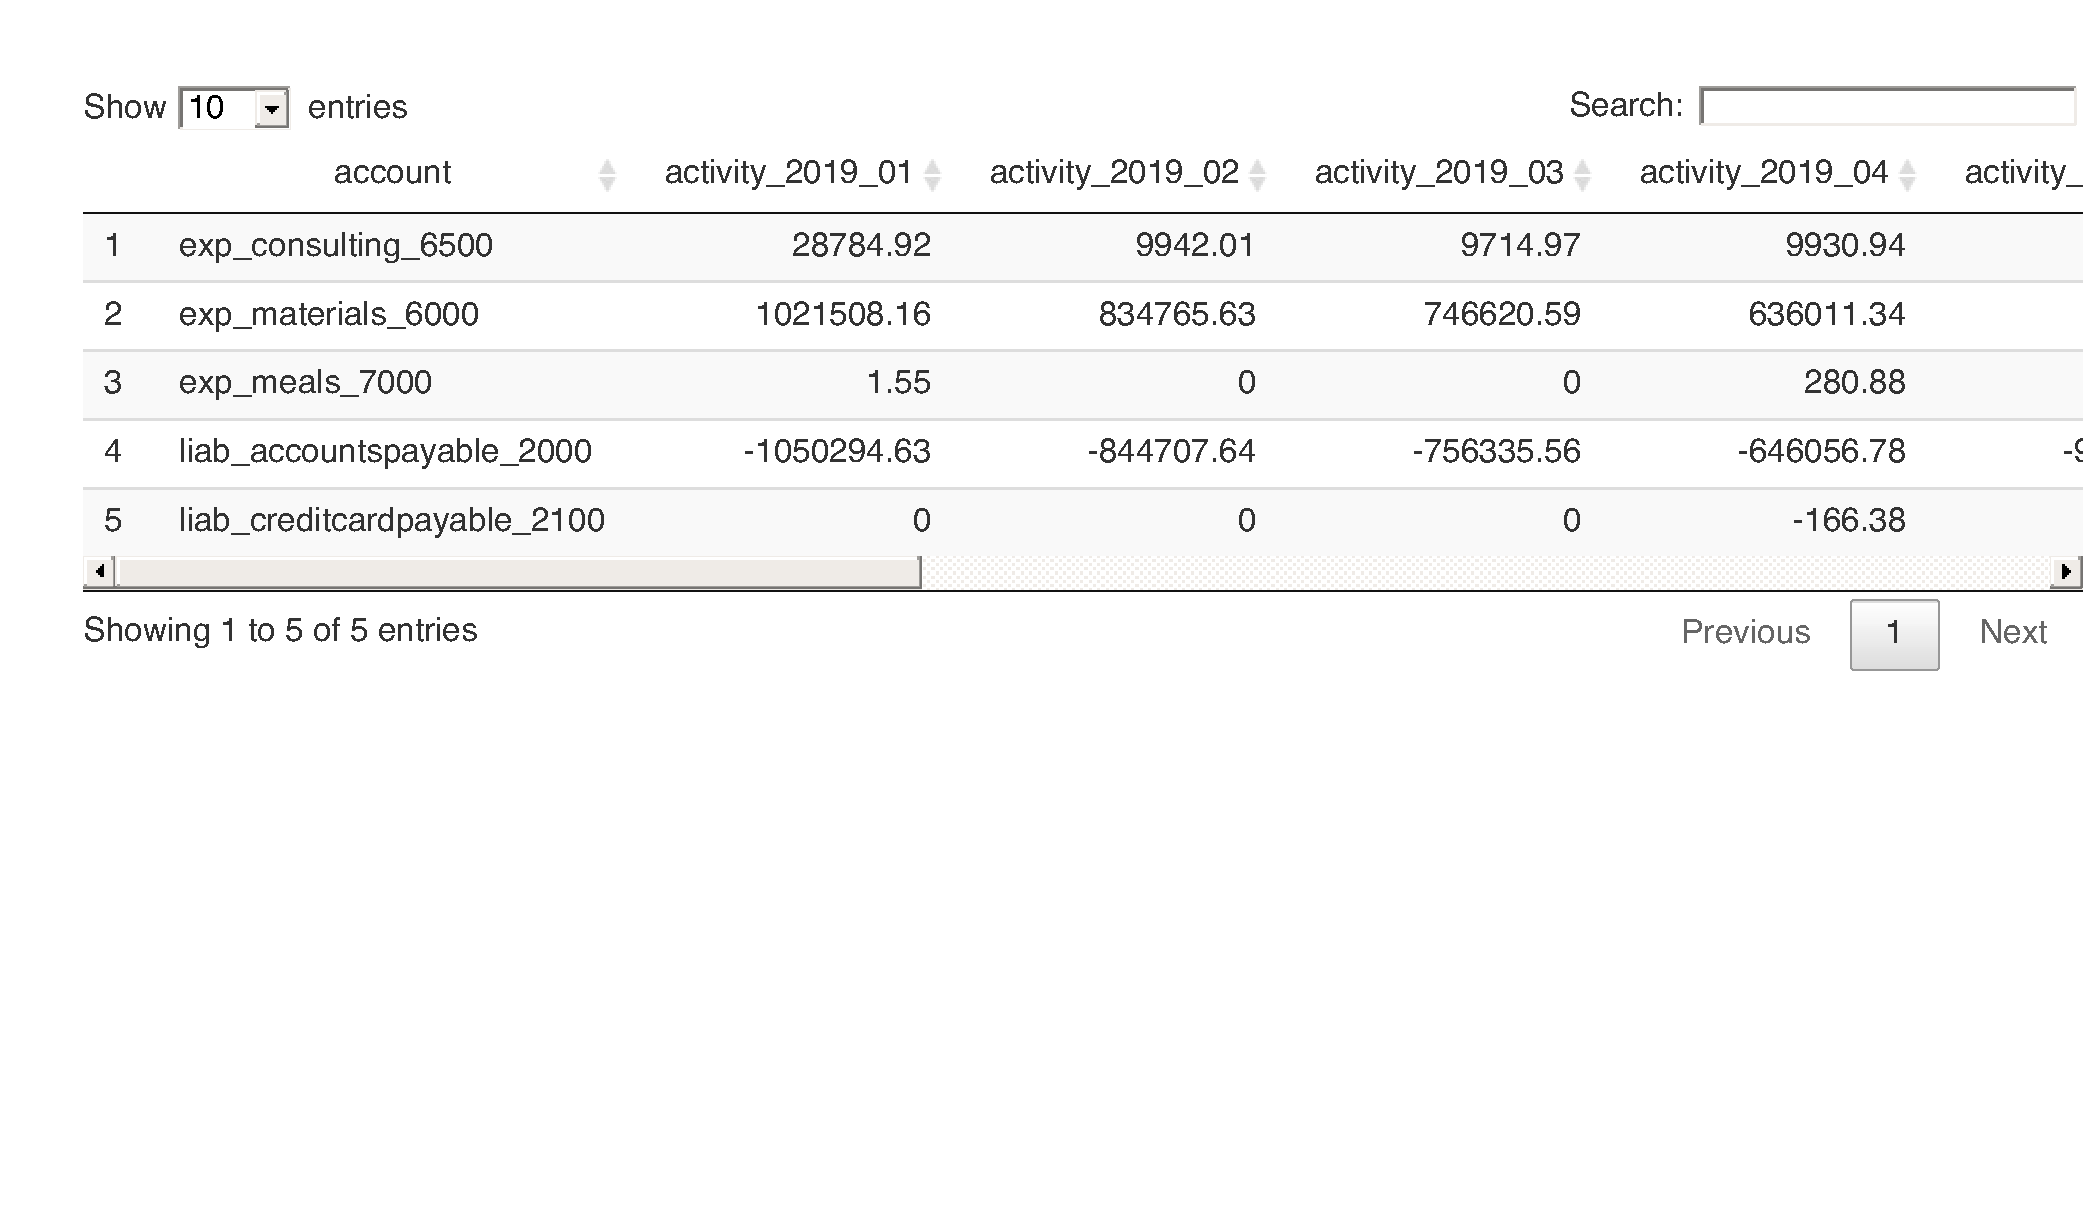
\includegraphics{Audit_Analytics_with-R_files/figure-latex/unnamed-chunk-39-1.pdf}

\begin{Shaded}
\begin{Highlighting}[]
\NormalTok{tb_long <-}\StringTok{ }\NormalTok{tb }\OperatorTok
\StringTok{  }\KeywordTok{pivot_longer}\NormalTok{(}\DataTypeTok{cols =} \KeywordTok{starts_with}\NormalTok{(}\StringTok{"activity_"}\NormalTok{), }\CommentTok{# We want to aggregate the values in these columns}
               \DataTypeTok{names_to =} \StringTok{"period"}\NormalTok{, }\CommentTok{# What we want to call this new column}
               \DataTypeTok{values_to =} \StringTok{"activity"}\NormalTok{) }\CommentTok{# And the values we want to take from it}

\NormalTok{tb_long}
\end{Highlighting}
\end{Shaded}

\begin{verbatim}
## # A tibble: 60 x 3
##    account             period           activity
##    <chr>               <chr>               <dbl>
##  1 exp_consulting_6500 activity_2019_01   28785.
##  2 exp_consulting_6500 activity_2019_02    9942.
##  3 exp_consulting_6500 activity_2019_03    9715.
##  4 exp_consulting_6500 activity_2019_04    9931.
##  5 exp_consulting_6500 activity_2019_05   28973.
##  6 exp_consulting_6500 activity_2019_06   37677.
##  7 exp_consulting_6500 activity_2019_07   19295.
##  8 exp_consulting_6500 activity_2019_08    9104.
##  9 exp_consulting_6500 activity_2019_09   28698.
## 10 exp_consulting_6500 activity_2019_10   28753.
## # ... with 50 more rows
\end{verbatim}

This data is now represented longer - there is now one unique value (activity) for each account and month. From here, we can now \texttt{summarize()}:

\begin{Shaded}
\begin{Highlighting}[]
\NormalTok{tb_long }\OperatorTok
\StringTok{  }\KeywordTok{group_by}\NormalTok{(account) }\OperatorTok
\StringTok{  }\KeywordTok{summarize}\NormalTok{(}\DataTypeTok{tb_activity =} \KeywordTok{sum}\NormalTok{(activity))}
\end{Highlighting}
\end{Shaded}

\begin{verbatim}
## `summarise()` ungrouping output (override with `.groups` argument)
\end{verbatim}

\begin{verbatim}
## # A tibble: 5 x 2
##   account                     tb_activity
##   <chr>                             <dbl>
## 1 exp_consulting_6500             248427.
## 2 exp_materials_6000             9984507.
## 3 exp_meals_7000                    1706.
## 4 liab_accountspayable_2000    -10227945.
## 5 liab_creditcardpayable_2100      -6695.
\end{verbatim}

While any of these approaches will work to calculate the trial balance of activity, there are sustainability advantages where the columns are not verbatim and explicitly mentioned - what matters is how you believe your dataset can change over time, or how easily readable you can communicate your work to a new individual.

\hypertarget{asserting-completeness}{%
\section{Asserting Completeness}\label{asserting-completeness}}

The practical goal before we do any further testing is to ensure we're not wasting time with a data set that is missing information. This completeness test will help validate that we received data for twelve months of GL activity. In Journal Entry testing, this means we will compare the summarized Trial Balance file against the General Ledger entries to obtain reasonableness that our data set we received is complete.

To compare both the GL and TB, we will want to aggregate the data in both datasets before joining them together. First, we will aggregate the GL:

\begin{Shaded}
\begin{Highlighting}[]
\NormalTok{gl_summarized <-}\StringTok{ }\NormalTok{gl }\OperatorTok
\StringTok{  }\KeywordTok{group_by}\NormalTok{(account) }\OperatorTok
\StringTok{  }\KeywordTok{summarize}\NormalTok{(}\DataTypeTok{gl_total =} \KeywordTok{sum}\NormalTok{(amount),}
           \DataTypeTok{.groups =} \StringTok{'drop'}\NormalTok{) }\CommentTok{# Needed to suppress the ungrouping object message}

\NormalTok{gl_summarized}
\end{Highlighting}
\end{Shaded}

\begin{verbatim}
## # A tibble: 5 x 2
##   account                       gl_total
##   <chr>                            <dbl>
## 1 exp_consulting_6500            248427.
## 2 exp_materials_6000            9984507.
## 3 exp_meals_7000                   1706.
## 4 liab_accountspayable_2000   -10227945.
## 5 liab_creditcardpayable_2100     -6695.
\end{verbatim}

And also aggregate the TB:

\begin{Shaded}
\begin{Highlighting}[]
\NormalTok{tb_summarized <-}\StringTok{ }\NormalTok{tb }\OperatorTok
\StringTok{  }\KeywordTok{mutate}\NormalTok{(}\DataTypeTok{tb_activity =} \KeywordTok{rowSums}\NormalTok{(}
    \KeywordTok{select}\NormalTok{(., }\KeywordTok{contains}\NormalTok{(}\StringTok{'activity_'}\NormalTok{))}
\NormalTok{    )) }\OperatorTok
\StringTok{  }\KeywordTok{select}\NormalTok{(account, tb_activity)}

\NormalTok{tb_summarized}
\end{Highlighting}
\end{Shaded}

\begin{verbatim}
## # A tibble: 5 x 2
##   account                     tb_activity
##   <chr>                             <dbl>
## 1 exp_consulting_6500             248427.
## 2 exp_materials_6000             9984507.
## 3 exp_meals_7000                    1706.
## 4 liab_accountspayable_2000    -10227945.
## 5 liab_creditcardpayable_2100      -6695.
\end{verbatim}

\hypertarget{completeness-join}{%
\subsection{Joining the GL to the TB}\label{completeness-join}}

To perform a proper test of completeness, we should join both tables together. \emph{dplyr} and the \texttt{*\_join()} family of functions can be used to join tables, and also used as diagnosis tools to help debug information as well.

Our GL and TB summarized datasets could be joined by the \texttt{account} column, prior to performing the calculation to identify differences:

\begin{Shaded}
\begin{Highlighting}[]
\NormalTok{gl_summarized }\OperatorTok
\StringTok{  }\KeywordTok{full_join}\NormalTok{(tb_summarized, }\DataTypeTok{by =} \StringTok{'account'}\NormalTok{)}
\end{Highlighting}
\end{Shaded}

\begin{verbatim}
## # A tibble: 5 x 3
##   account                       gl_total tb_activity
##   <chr>                            <dbl>       <dbl>
## 1 exp_consulting_6500            248427.     248427.
## 2 exp_materials_6000            9984507.    9984507.
## 3 exp_meals_7000                   1706.       1706.
## 4 liab_accountspayable_2000   -10227945.  -10227945.
## 5 liab_creditcardpayable_2100     -6695.      -6695.
\end{verbatim}

Once you have joined the columns together, a simple difference calculation will let you know what the differences are (if any):

\begin{Shaded}
\begin{Highlighting}[]
\NormalTok{gl_summarized }\OperatorTok
\StringTok{  }\KeywordTok{full_join}\NormalTok{(tb_summarized, }\DataTypeTok{by =} \StringTok{'account'}\NormalTok{) }\OperatorTok
\StringTok{  }\KeywordTok{mutate}\NormalTok{(}\DataTypeTok{tb_diff =}\NormalTok{ gl_total }\OperatorTok{-}\StringTok{ }\NormalTok{tb_activity)}
\end{Highlighting}
\end{Shaded}

\begin{verbatim}
## # A tibble: 5 x 4
##   account                       gl_total tb_activity tb_diff
##   <chr>                            <dbl>       <dbl>   <dbl>
## 1 exp_consulting_6500            248427.     248427.       0
## 2 exp_materials_6000            9984507.    9984507.       0
## 3 exp_meals_7000                   1706.       1706.       0
## 4 liab_accountspayable_2000   -10227945.  -10227945.       0
## 5 liab_creditcardpayable_2100     -6695.      -6695.       0
\end{verbatim}

And if you like clean working papers, simply filter to identify where the reconciliation did not work out:

\begin{Shaded}
\begin{Highlighting}[]
\NormalTok{gl_summarized }\OperatorTok
\StringTok{  }\KeywordTok{full_join}\NormalTok{(tb_summarized, }\DataTypeTok{by =} \StringTok{'account'}\NormalTok{) }\OperatorTok
\StringTok{  }\KeywordTok{mutate}\NormalTok{(}\DataTypeTok{tb_diff =}\NormalTok{ gl_total }\OperatorTok{-}\StringTok{ }\NormalTok{tb_activity) }\OperatorTok
\StringTok{  }\NormalTok{dplyr}\OperatorTok{::}\KeywordTok{filter}\NormalTok{(tb_diff }\OperatorTok{!=}\StringTok{ }\DecValTok{0}\NormalTok{)}
\end{Highlighting}
\end{Shaded}

\begin{verbatim}
## # A tibble: 0 x 4
## # ... with 4 variables: account <chr>, gl_total <dbl>, tb_activity <dbl>,
## #   tb_diff <dbl>
\end{verbatim}

\hypertarget{cautionary-notes-for-completeness}{%
\section{Cautionary notes for Completeness}\label{cautionary-notes-for-completeness}}

While performing completeness, you are proving you have a complete set of data. Exercise caution and ensure you are aware of the following:

\begin{itemize}
\item
  A completeness check is only as good as the data provided. In the above case, if November was completely excluded in both GL and TB, you would not be able to detect it at this stage if you did not look through the TB data to see that all twelve months were included.
\item
  Using \texttt{*\_join()} functions will generally return all combinations of matches. This is a strong motivation to ensure you have summarized rows by the join columns, prior to joining. Once you have summarized your data, the \texttt{*\_join()} functions are far more predictable.
\item
  \texttt{full\_join()} will indicate if there are any accounts missing from either table. In our example, if the \texttt{tb\_summarized} data had missing accounts that did exist in the \texttt{gl\_summarized} table, the resulting \texttt{tb\_activity} column values would show up as NA.
\item
  \texttt{anti\_join()} will show what columns are included on the left, but missing on the right. In our example, if the \texttt{tb\_summarized} data had missing accounts that existed in the \texttt{gl\_summarized} table, only this account would show up in the results.
\end{itemize}

You may want to consider testing for invalid values or missing dates up front. While the primary goal is to ensure the datasets received are appropriate, you may want to consider validating this information earlier. The next chapter will show you how to further manipulate and test these columns.

\hypertarget{cleaning-data}{%
\chapter{Cleaning data}\label{cleaning-data}}

Cleaning a data set, including fields and reshaping of the data, is a fundamental skill in order to get the data into an analyzable format. Real world data is messy, and will not typically be immediately analyzable immediately after downloading.

For this section we will still use the company database, along with some more packages. New packages in this chapter include lubridate and tidyr.

\begin{Shaded}
\begin{Highlighting}[]
\KeywordTok{library}\NormalTok{(dplyr) }\CommentTok{# For manipulating data}
\KeywordTok{library}\NormalTok{(tidyr) }\CommentTok{# For making data long and wide}

\KeywordTok{library}\NormalTok{(lubridate) }\CommentTok{# For date handling}

\KeywordTok{library}\NormalTok{(DBI) }\CommentTok{# For database connections}

\KeywordTok{dir.create}\NormalTok{(}\StringTok{"data"}\NormalTok{, }\DataTypeTok{showWarnings =} \OtherTok{FALSE}\NormalTok{)}

\KeywordTok{download.file}\NormalTok{(}\DataTypeTok{url =} \StringTok{"https://github.com/jonlinca/auditanalytics/raw/master/data/rauditanalytics.sqlite"}\NormalTok{,}
             \DataTypeTok{destfile =} \StringTok{"data/rauditanalytics.sqlite"}\NormalTok{, }\DataTypeTok{mode =} \StringTok{"wb"}\NormalTok{)}

\NormalTok{con <-}\StringTok{ }\KeywordTok{dbConnect}\NormalTok{(RSQLite}\OperatorTok{::}\KeywordTok{SQLite}\NormalTok{(), }\StringTok{"data/rauditanalytics.sqlite"}\NormalTok{)}

\NormalTok{gl <-}\StringTok{ }\KeywordTok{tbl}\NormalTok{(con, }\StringTok{'gl'}\NormalTok{) }\OperatorTok
\StringTok{  }\KeywordTok{collect}\NormalTok{()}

\NormalTok{vendors <-}\StringTok{ }\KeywordTok{tbl}\NormalTok{(con, }\StringTok{'vendors'}\NormalTok{) }\OperatorTok
\StringTok{  }\KeywordTok{collect}\NormalTok{()}

\NormalTok{industry <-}\StringTok{ }\KeywordTok{dbReadTable}\NormalTok{(con, }\StringTok{'industry'}\NormalTok{) }\OperatorTok
\StringTok{  }\KeywordTok{collect}\NormalTok{()}

\KeywordTok{dbDisconnect}\NormalTok{(con)}
\end{Highlighting}
\end{Shaded}

\hypertarget{basic-math}{%
\section{Basic math}\label{basic-math}}

We covered some of the basic operators in R in the Completeness chapter, so we'll cover some more calculations and transformations.

\begin{Shaded}
\begin{Highlighting}[]
\NormalTok{x <-}\StringTok{ }\KeywordTok{c}\NormalTok{(}\DecValTok{1}\NormalTok{, }\DecValTok{2}\NormalTok{, }\DecValTok{3}\NormalTok{)}
\NormalTok{y <-}\StringTok{ }\KeywordTok{c}\NormalTok{(}\DecValTok{4}\NormalTok{, }\DecValTok{5}\NormalTok{, }\DecValTok{6}\NormalTok{)}
\end{Highlighting}
\end{Shaded}

The basic mathematical symbols will calculate a vector with a position element against a different vector with the same position. In this case, the first number in \texttt{x} is added to the first number in \texttt{y} resulting in the first calculation, the second number in \texttt{x} is added to the second number in \texttt{y} resulting in the second calculation, and so on.

\begin{Shaded}
\begin{Highlighting}[]
\NormalTok{y }\OperatorTok{+}\StringTok{ }\NormalTok{x}
\end{Highlighting}
\end{Shaded}

\begin{verbatim}
## [1] 5 7 9
\end{verbatim}

This distinction is important - vectorization allows R to be fast, but it changes how the user needs to understand objects.

\texttt{sum()} is fairly straight forward - it will add all the elements given, together:

\begin{Shaded}
\begin{Highlighting}[]
\KeywordTok{sum}\NormalTok{(x)}
\end{Highlighting}
\end{Shaded}

\begin{verbatim}
## [1] 6
\end{verbatim}

If you specify multiple vectors - it will merely combine them all together, equivalent to \texttt{sum(c(1,\ 2,\ 3),\ c(4,\ 5,\ 6))}:

\begin{Shaded}
\begin{Highlighting}[]
\KeywordTok{sum}\NormalTok{(x, y)}
\end{Highlighting}
\end{Shaded}

\begin{verbatim}
## [1] 21
\end{verbatim}

We mentioned in the prior chapter about NA values, which were `Not Available' or Missing Values. It becomes important to understand the implication of them in your calculations. For example, when a NA value exists in a vector, you will get an NA by default:

\begin{Shaded}
\begin{Highlighting}[]
\NormalTok{z <-}\StringTok{ }\KeywordTok{c}\NormalTok{(}\DecValTok{1}\NormalTok{, }\DecValTok{2}\NormalTok{, }\OtherTok{NA}\NormalTok{)}
\KeywordTok{sum}\NormalTok{(z)}
\end{Highlighting}
\end{Shaded}

\begin{verbatim}
## [1] NA
\end{verbatim}

While \texttt{sum()}, and several other functions like \texttt{mean()}, \texttt{min()} and \texttt{max()} all generally behave in predictable manners, they all have an argument of \texttt{na.rm\ =\ FALSE} by default (enter \texttt{?sum} to see this argument in the help file. The reason why \texttt{FALSE} is by default is that it brings attention to the vector missing values. If you want to perform the calculation on this, you either need to substitute the \texttt{NA} out for a value (imputation), or simply ignore them. Both these decisions require professional judgment before substitution or ignoring. To substitute \texttt{NA} for a value (for example, 10):

\begin{Shaded}
\begin{Highlighting}[]
\KeywordTok{is.na}\NormalTok{(z) }\CommentTok{# Shows which positions in the vector have an NA value}
\end{Highlighting}
\end{Shaded}

\begin{verbatim}
## [1] FALSE FALSE  TRUE
\end{verbatim}

\begin{Shaded}
\begin{Highlighting}[]
\NormalTok{z[}\KeywordTok{is.na}\NormalTok{(z)] <-}\StringTok{ }\DecValTok{10} \CommentTok{# Where the z value is is.na, assign 10}
\KeywordTok{sum}\NormalTok{(z)}
\end{Highlighting}
\end{Shaded}

\begin{verbatim}
## [1] 13
\end{verbatim}

Or alternatively, set the argument \texttt{na.rm\ =\ TRUE} to throw away these values completely:

\begin{Shaded}
\begin{Highlighting}[]
\NormalTok{z <-}\StringTok{ }\KeywordTok{c}\NormalTok{(}\DecValTok{1}\NormalTok{, }\DecValTok{2}\NormalTok{, }\OtherTok{NA}\NormalTok{)}
\KeywordTok{sum}\NormalTok{(z, }\DataTypeTok{na.rm =} \OtherTok{TRUE}\NormalTok{)}
\end{Highlighting}
\end{Shaded}

\begin{verbatim}
## [1] 3
\end{verbatim}

\hypertarget{dates-and-times}{%
\section{Dates and Times}\label{dates-and-times}}

Unlike numbers, date and times are inherently more complex. They require many additional considerations to properly wrangle:

\begin{itemize}
\tightlist
\item
  What format is the date and time in?
\item
  Are the timezones as expected? This also applies for dates.
\item
  Do you want the the month the transaction took place in? The year? The day-of-week?
\item
  Do you care about daylight savings time?
\end{itemize}

Starting with a basic example, lets understand the basic characteristics of dates. When you define a new date, the \texttt{lubridate::as\_date()} function (or base \texttt{as.Date()}) works to convert character strings to dates.

\begin{Shaded}
\begin{Highlighting}[]
\NormalTok{startString <-}\StringTok{ '2020-07-30'} \CommentTok{# ISO 8601 standards, follow them}

\CommentTok{# base::as.Date(startString) # Same thing as as_date, for now...}
\NormalTok{start <-}\StringTok{ }\NormalTok{lubridate}\OperatorTok{::}\KeywordTok{as_date}\NormalTok{(startString)}

\KeywordTok{class}\NormalTok{(start)}
\end{Highlighting}
\end{Shaded}

\begin{verbatim}
## [1] "Date"
\end{verbatim}

You can convert any date to a date, as long as you specify the mask or format. A mask specifies where the date, month, year exist (as well as for time, hours, minutes, seconds). If you check the help file for \texttt{?strptime}, you will see several different formats for both specifying dates and times. For example, \texttt{\%Y} is a four digit year while \texttt{\%y\%} is a two digit year. Here are a few examples with the same date (some are more unreasonable than others, but all can be captured):

\begin{Shaded}
\begin{Highlighting}[]
\NormalTok{lubridate}\OperatorTok{::}\KeywordTok{as_date}\NormalTok{(}\StringTok{'2020-07-30'}\NormalTok{, }\DataTypeTok{format =} \StringTok{"%Y-%m-%d"}\NormalTok{)}
\NormalTok{lubridate}\OperatorTok{::}\KeywordTok{as_date}\NormalTok{(}\StringTok{'30/07/2020'}\NormalTok{, }\DataTypeTok{format =} \StringTok{"%d/%m/%Y"}\NormalTok{) }\CommentTok{# Not ISO 8601}
\NormalTok{lubridate}\OperatorTok{::}\KeywordTok{as_date}\NormalTok{(}\StringTok{'July 30, 20'}\NormalTok{, }\DataTypeTok{format =} \StringTok{"%B %d, %y"}\NormalTok{) }\CommentTok{# Really not ISO 8601}
\NormalTok{lubridate}\OperatorTok{::}\KeywordTok{as_date}\NormalTok{(}\StringTok{'Jul3020'}\NormalTok{, }\DataTypeTok{format =} \StringTok{"%b%d%y"}\NormalTok{) }\CommentTok{# Definitely not ISO 8601}
\end{Highlighting}
\end{Shaded}

The same concept also applies to datetimes, where you can convert a given time to a `POSIXct' or `POSIXlt' format (the differences between `POSIXct' and `POSIXlt' are found in \texttt{?DateTimeClasses}, under details):

\begin{Shaded}
\begin{Highlighting}[]
\NormalTok{starttime_base <-}\StringTok{ }\KeywordTok{as.POSIXct}\NormalTok{(}\StringTok{'2020-07-30 12:00:00'}\NormalTok{)}
\NormalTok{starttime_lub <-}\StringTok{ }\NormalTok{lubridate}\OperatorTok{::}\KeywordTok{as_datetime}\NormalTok{(}\StringTok{'2020-07-30 12:00:00'}\NormalTok{)}

\KeywordTok{class}\NormalTok{(starttime_base); }\KeywordTok{class}\NormalTok{(starttime_lub)}
\end{Highlighting}
\end{Shaded}

\begin{verbatim}
## [1] "POSIXct" "POSIXt"
\end{verbatim}

\begin{verbatim}
## [1] "POSIXct" "POSIXt"
\end{verbatim}

And format masks apply as well to date time, just in case you get something unconventional:

\begin{Shaded}
\begin{Highlighting}[]
\NormalTok{lubridate}\OperatorTok{::}\KeywordTok{as_datetime}\NormalTok{(}\StringTok{'2020-07-30 12:00:00 PM -0600'}\NormalTok{, }
                       \DataTypeTok{format =} \StringTok{"%Y-%m-%d %I:%M:%S %p %z"}\NormalTok{)}
\end{Highlighting}
\end{Shaded}

\begin{verbatim}
## [1] "2020-07-30 18:00:00 UTC"
\end{verbatim}

\hypertarget{understanding-default-time-zones}{%
\subsection{Understanding Default Time Zones}\label{understanding-default-time-zones}}

Did you consider the time zone that the times were created in? This is system-specific and base \texttt{POSIXct} and lubridate \texttt{as\_datetime} behave differently, so you have to be careful!

\begin{Shaded}
\begin{Highlighting}[]
\KeywordTok{print}\NormalTok{(starttime_base); }\KeywordTok{attr}\NormalTok{(starttime_base,}\StringTok{"tzone"}\NormalTok{)}
\end{Highlighting}
\end{Shaded}

\begin{verbatim}
## [1] "2020-07-30 12:00:00 MDT"
\end{verbatim}

\begin{verbatim}
## [1] ""
\end{verbatim}

Notice that base treats the creation of the current timezone based off your local R machine, although its not extractable (and you will eventually find, hard to change).

\begin{Shaded}
\begin{Highlighting}[]
\KeywordTok{print}\NormalTok{(starttime_lub); }\KeywordTok{tz}\NormalTok{(starttime_lub)}
\end{Highlighting}
\end{Shaded}

\begin{verbatim}
## [1] "2020-07-30 12:00:00 UTC"
\end{verbatim}

\begin{verbatim}
## [1] "UTC"
\end{verbatim}

The lubridate version will assign the date-time automatically to UTC, unless you specify it. It is for this reason you will generally want to avoid using base R to convert to date times, and stick with lubridate for better predictability.

Having an automatic conversion to UTC isn't bad per se - having a universal ground truth to UTC is good, as it removes Daylight Saving component, and is an easy way to standardize multiple data sets together. Unfortunately, many systems will not tell you what time zone their data is in, so you will have to figure it out and ensure R is aligned accordingly.

\hypertarget{override-or-display-timezones}{%
\subsection{Override or display timezones}\label{override-or-display-timezones}}

Hopefully you have been convinced to stick with lubridate for your date transformations. Now, lets get some confidence on these timezone transformations.

The first method is \texttt{force\_tz()}, which forces the current time to become that same hour in a new timezone. When we assigned July 30th to the date, we would have assumed this date would have been in the current timezone we exist in (generally, the system time-zone you are in). To do this, specify the date, but also the time zone you want the date or time to be harmonized in:

\begin{Shaded}
\begin{Highlighting}[]
\NormalTok{starttime_lub }\CommentTok{# Starts as UTC}
\end{Highlighting}
\end{Shaded}

\begin{verbatim}
## [1] "2020-07-30 12:00:00 UTC"
\end{verbatim}

\begin{Shaded}
\begin{Highlighting}[]
\KeywordTok{force_tz}\NormalTok{(starttime_lub, }\DataTypeTok{tz =} \StringTok{'Canada/Mountain'}\NormalTok{) }\CommentTok{# Force the saved time to be Mountain}
\end{Highlighting}
\end{Shaded}

\begin{verbatim}
## [1] "2020-07-30 12:00:00 MDT"
\end{verbatim}

Alternatively, you may wish to only convert the time so its displayed in the correct timezone, but leave the base truth as is. \texttt{with\_tz()} will allow you to change the timezone that is displayed, while honoring the original time in the data.

\begin{Shaded}
\begin{Highlighting}[]
\NormalTok{starttime_lub}
\end{Highlighting}
\end{Shaded}

\begin{verbatim}
## [1] "2020-07-30 12:00:00 UTC"
\end{verbatim}

\begin{Shaded}
\begin{Highlighting}[]
\KeywordTok{with_tz}\NormalTok{(starttime_lub, }\DataTypeTok{tz =} \StringTok{'Canada/Mountain'}\NormalTok{) }\CommentTok{# Display the current time as Mountain}
\end{Highlighting}
\end{Shaded}

\begin{verbatim}
## [1] "2020-07-30 06:00:00 MDT"
\end{verbatim}

\hypertarget{daylight-saving-implications}{%
\subsection{Daylight Saving Implications}\label{daylight-saving-implications}}

There are also timezone implications when it comes to daylight saving time. This is especially important when making audit decisions based on duration, or expected local norms for time-of-day.

In several locales across the world, daylight saving time will alter the clock for half a year locally, but has no impact on UTC. For example, your staff may start their day at 8:00 AM locally. When daylight saving kicks in, the local time stays at 8:00 AM and the UTC time shifts from 15:00 to 14:00.

\begin{Shaded}
\begin{Highlighting}[]
\NormalTok{pre <-}\StringTok{ }\KeywordTok{as_datetime}\NormalTok{(}\StringTok{'2020-03-07 8:00:00'}\NormalTok{, }\DataTypeTok{tz =} \StringTok{'Canada/Mountain'}\NormalTok{) }\CommentTok{# The day before DST starts}
\NormalTok{post <-}\StringTok{ }\KeywordTok{as_datetime}\NormalTok{(}\StringTok{'2020-03-08 8:00:00'}\NormalTok{, }\DataTypeTok{tz =} \StringTok{'Canada/Mountain'}\NormalTok{) }\CommentTok{# The day DST started}

\KeywordTok{dst}\NormalTok{(pre); }\KeywordTok{with_tz}\NormalTok{(pre, }\DataTypeTok{tz =} \StringTok{'UTC'}\NormalTok{) }\CommentTok{# Was DST active before? ; What is the UTC time before? }
\end{Highlighting}
\end{Shaded}

\begin{verbatim}
## [1] FALSE
\end{verbatim}

\begin{verbatim}
## [1] "2020-03-07 15:00:00 UTC"
\end{verbatim}

\begin{Shaded}
\begin{Highlighting}[]
\KeywordTok{dst}\NormalTok{(post); }\KeywordTok{with_tz}\NormalTok{(post, }\DataTypeTok{tz =} \StringTok{'UTC'}\NormalTok{) }\CommentTok{# Was DST active after? ; What is the UTC time after?}
\end{Highlighting}
\end{Shaded}

\begin{verbatim}
## [1] TRUE
\end{verbatim}

\begin{verbatim}
## [1] "2020-03-08 14:00:00 UTC"
\end{verbatim}

\hypertarget{differences-between-time}{%
\subsection{Differences between time}\label{differences-between-time}}

Another common calculation is to calculate the time differences between two points of time. This seemingly simple action has several interpretations behind it. Do you want relative dates? Do you want exact elapsed time?

\begin{quote}
People are not always consistent in how they expect time to behave. Sometimes the passage of time is a monotone progression of instants that should be as mathematically reliable as the number line. On other occasions time must follow complex conventions and rules so that the clock times we see reflect what we expect to observe in terms of daylight, season, and congruence with the atomic clock. (Vitalie Spinu \protect\hyperlink{ref-lubridate-help}{2016})
\end{quote}

Adding time is easy - you simply need to decide if you're adding a period (i.e.~human construct of days) or if you are following physical time (i.e.~seconds). The main difference is choosing lubridate's functions that honor periods or durations

\begin{Shaded}
\begin{Highlighting}[]
\NormalTok{pre <-}\StringTok{ }\KeywordTok{as_datetime}\NormalTok{(}\StringTok{'2020-03-07 8:00:00'}\NormalTok{, }\DataTypeTok{tz =} \StringTok{'Canada/Mountain'}\NormalTok{) }\CommentTok{# The day before DST starts}
\NormalTok{post <-}\StringTok{ }\KeywordTok{as_datetime}\NormalTok{(}\StringTok{'2020-03-08 8:00:00'}\NormalTok{, }\DataTypeTok{tz =} \StringTok{'Canada/Mountain'}\NormalTok{) }\CommentTok{# The day DST started, skipped ahead 1 hour}

\CommentTok{# Periods: Human construct of days}
\NormalTok{pre }\OperatorTok{+}\StringTok{ }\KeywordTok{days}\NormalTok{(}\DecValTok{1}\NormalTok{) ; pre }\OperatorTok{+}\StringTok{ }\KeywordTok{hours}\NormalTok{(}\DecValTok{24}\NormalTok{) }\CommentTok{# Equal to post, the human construct}
\end{Highlighting}
\end{Shaded}

\begin{verbatim}
## [1] "2020-03-08 08:00:00 MDT"
\end{verbatim}

\begin{verbatim}
## [1] "2020-03-08 08:00:00 MDT"
\end{verbatim}

\begin{Shaded}
\begin{Highlighting}[]
\CommentTok{# Duration: Physical construct of time}
\NormalTok{pre }\OperatorTok{+}\StringTok{ }\KeywordTok{ddays}\NormalTok{(}\DecValTok{1}\NormalTok{) ; pre }\OperatorTok{+}\StringTok{ }\KeywordTok{dhours}\NormalTok{(}\DecValTok{24}\NormalTok{) }\CommentTok{# NOT to post, but actually 1 hour after}
\end{Highlighting}
\end{Shaded}

\begin{verbatim}
## [1] "2020-03-08 09:00:00 MDT"
\end{verbatim}

\begin{verbatim}
## [1] "2020-03-08 09:00:00 MDT"
\end{verbatim}

Calculating intervals and periods is a bit different. If we go back up to our example of pre-and-post daylight saving time, we can either expect this answer to be 1 day or 23 hours. Again, depending on your use case, it is up to you.\footnote{Division is the intended mechanism - see \url{https://github.com/tidyverse/lubridate/issues/105} and \url{https://stackoverflow.com/questions/8765621/length-of-lubridate-interval}}

\begin{Shaded}
\begin{Highlighting}[]
\NormalTok{span <-}\StringTok{ }\KeywordTok{interval}\NormalTok{(pre, post)}

\CommentTok{# Period: To find the number of days, in human constructs}
\NormalTok{span }\OperatorTok{/}\StringTok{ }\KeywordTok{days}\NormalTok{(}\DecValTok{1}\NormalTok{) }\CommentTok{# Period calculation by days. }
\end{Highlighting}
\end{Shaded}

\begin{verbatim}
## [1] 1
\end{verbatim}

\begin{Shaded}
\begin{Highlighting}[]
\CommentTok{# Duration - To find the hours between, in physical constructs}
\KeywordTok{as.duration}\NormalTok{(span)}
\end{Highlighting}
\end{Shaded}

\begin{verbatim}
## [1] "82800s (~23 hours)"
\end{verbatim}

\hypertarget{derived-date-information}{%
\subsection{Derived date information}\label{derived-date-information}}

A common task for auditors is to find out the month a transaction took place in. With lubridate, its quite straight forward - for example, to extract the month, you don't need to have any messy substrings (or to extract other useful times, for that matter):

\begin{Shaded}
\begin{Highlighting}[]
\NormalTok{thedate <-}\StringTok{ }\KeywordTok{as_datetime}\NormalTok{(}\StringTok{'2020-07-01 12:00:00'}\NormalTok{, }\DataTypeTok{tz =} \StringTok{'Canada/Mountain'}\NormalTok{) }

\KeywordTok{month}\NormalTok{(thedate)}
\end{Highlighting}
\end{Shaded}

\begin{verbatim}
## [1] 7
\end{verbatim}

\begin{Shaded}
\begin{Highlighting}[]
\KeywordTok{year}\NormalTok{(thedate)}
\end{Highlighting}
\end{Shaded}

\begin{verbatim}
## [1] 2020
\end{verbatim}

\begin{Shaded}
\begin{Highlighting}[]
\KeywordTok{quarter}\NormalTok{(thedate) }\CommentTok{# Canada Day starts on the first day of the third quarter. Does your company Financial Year not start on January 1? Just change the fiscal_start argument.}
\end{Highlighting}
\end{Shaded}

\begin{verbatim}
## [1] 3
\end{verbatim}

\begin{Shaded}
\begin{Highlighting}[]
\KeywordTok{wday}\NormalTok{(thedate, }\DataTypeTok{label =} \OtherTok{TRUE}\NormalTok{)}
\end{Highlighting}
\end{Shaded}

\begin{verbatim}
## [1] Wed
## Levels: Sun < Mon < Tue < Wed < Thu < Fri < Sat
\end{verbatim}

\hypertarget{cleaning-numerical-dates}{%
\subsection{Cleaning numerical dates}\label{cleaning-numerical-dates}}

With dates, sometimes they may represented as a number - it is important to understand your source system date before you convert it.

Some systems may calculate a date from an `origin' using the number. While our concept of time may start with 0 AD (as the origin), several computer systems and applications do not behave in that manner. Excel, for example, starts from 1900-01-01, whereas Unix operating systems have their origin as 1970-01-01. If converting a date from a number, you need to research and then specify an origin, otherwise you will have challenges in specifying dates.

In our vendors table, we have a numeric date but also a date in a character form for reference

\begin{Shaded}
\begin{Highlighting}[]
\NormalTok{vendors }\OperatorTok
\StringTok{  }\KeywordTok{select}\NormalTok{(date_added, date_added_char)}
\end{Highlighting}
\end{Shaded}

\begin{verbatim}
## # A tibble: 9 x 2
##   date_added date_added_char
##        <dbl> <chr>          
## 1      16631 2015-07-15     
## 2      16644 2015-07-28     
## 3      16581 2015-05-26     
## 4      16578 2015-05-23     
## 5      16620 2015-07-04     
## 6      16652 2015-08-05     
## 7      16578 2015-05-23     
## 8      16620 2015-07-04     
## 9      16652 2015-08-05
\end{verbatim}

By specifying the origin a few different origins, we can see what the origin should have been in this case:

\begin{Shaded}
\begin{Highlighting}[]
\NormalTok{vendors }\OperatorTok
\StringTok{  }\KeywordTok{select}\NormalTok{(date_added, date_added_char) }\OperatorTok
\StringTok{  }\KeywordTok{mutate}\NormalTok{(}\DataTypeTok{date_added_unix =} \KeywordTok{as_date}\NormalTok{(date_added, }\DataTypeTok{origin =} \StringTok{'1970-01-01'}\NormalTok{),}
         \DataTypeTok{date_added_excel =} \KeywordTok{as_date}\NormalTok{(date_added, }\DataTypeTok{origin =} \StringTok{'1900-01-01'}\NormalTok{))}
\end{Highlighting}
\end{Shaded}

\begin{verbatim}
## # A tibble: 9 x 4
##   date_added date_added_char date_added_unix date_added_excel
##        <dbl> <chr>           <date>          <date>          
## 1      16631 2015-07-15      2015-07-15      1945-07-15      
## 2      16644 2015-07-28      2015-07-28      1945-07-28      
## 3      16581 2015-05-26      2015-05-26      1945-05-26      
## 4      16578 2015-05-23      2015-05-23      1945-05-23      
## 5      16620 2015-07-04      2015-07-04      1945-07-04      
## 6      16652 2015-08-05      2015-08-05      1945-08-05      
## 7      16578 2015-05-23      2015-05-23      1945-05-23      
## 8      16620 2015-07-04      2015-07-04      1945-07-04      
## 9      16652 2015-08-05      2015-08-05      1945-08-05
\end{verbatim}

Dates can also appear in a completely different format. Julian (also known as mainframe or ordinal) dates are an example, where the year is specified but the date is relative to January 1. So 212 days is either July 30 or 31, depending if it is a leap year or not.

\begin{Shaded}
\begin{Highlighting}[]
\NormalTok{lubridate}\OperatorTok{::}\KeywordTok{as_date}\NormalTok{(}\StringTok{'19212'}\NormalTok{, }\DataTypeTok{format =} \StringTok{"%y%j"}\NormalTok{)}
\end{Highlighting}
\end{Shaded}

\begin{verbatim}
## [1] "2019-07-31"
\end{verbatim}

\begin{Shaded}
\begin{Highlighting}[]
\NormalTok{lubridate}\OperatorTok{::}\KeywordTok{as_date}\NormalTok{(}\StringTok{'20212'}\NormalTok{, }\DataTypeTok{format =} \StringTok{"%y%j"}\NormalTok{)}
\end{Highlighting}
\end{Shaded}

\begin{verbatim}
## [1] "2020-07-30"
\end{verbatim}

JDE E1's dates also add an extra digit in front of it, to symbolize the century. While there is no R way to translate 0 to 19xx and 1 to 20xx, practically speaking we are safe with assuming the century as we are at least 20 years past that point (as of this writing). Amending the mask to ignore the 1 can be done in the format:

\begin{Shaded}
\begin{Highlighting}[]
\NormalTok{lubridate}\OperatorTok{::}\KeywordTok{as_date}\NormalTok{(}\StringTok{'119212'}\NormalTok{, }\DataTypeTok{format =} \StringTok{"1%y%j"}\NormalTok{)}
\end{Highlighting}
\end{Shaded}

\begin{verbatim}
## [1] "2019-07-31"
\end{verbatim}

\begin{Shaded}
\begin{Highlighting}[]
\NormalTok{lubridate}\OperatorTok{::}\KeywordTok{as_date}\NormalTok{(}\StringTok{'120212'}\NormalTok{, }\DataTypeTok{format =} \StringTok{"1%y%j"}\NormalTok{)}
\end{Highlighting}
\end{Shaded}

\begin{verbatim}
## [1] "2020-07-30"
\end{verbatim}

\hypertarget{separate}{%
\section{Separate}\label{separate}}

Occasionally, distinct data will be combined in the same cell. This can be due to data entry or an unusual method of storing information. There will generally a separator within the field (similar to a delimiter), but the data is still contained within one field.

For example, if we look at our vendor table and \texttt{name} column, we can see the company names appear to also have a Contact person.

\begin{Shaded}
\begin{Highlighting}[]
\NormalTok{vendors }\OperatorTok
\StringTok{  }\KeywordTok{select}\NormalTok{(type, name)}
\end{Highlighting}
\end{Shaded}

\begin{verbatim}
## # A tibble: 9 x 2
##   type  name                                          
##   <chr> <chr>                                         
## 1 E     al-Bangura, Habeeba                           
## 2 E     Akina, Duncan                                 
## 3 E     el-Kazmi, Muneefa                             
## 4 V     el-Shafi Company Ltd - Contact: Rivera, Evan  
## 5 V     Bray Company Ltd - Contact: el-Jaffer, Shaheer
## 6 V     Chrisman Company Ltd - Contact: Burch, Kryslyn
## 7 V     el-Shafi Company Ltd - Contact: Rivera, Evan  
## 8 V     Bray Company Ltd - Contact: el-Jaffer, Shaheer
## 9 V     Chrisman Company Ltd - Contact: Burch, Kryslyn
\end{verbatim}

While the name is accurate, the contact name shouldn't be in there. We can isolate the contact name by using \texttt{separate()}, allowing us to split a column by defining a separator and also new column names. In this case, the `-' (dash) character could work:

\begin{Shaded}
\begin{Highlighting}[]
\NormalTok{vendors }\OperatorTok
\StringTok{  }\KeywordTok{select}\NormalTok{(type, name) }\OperatorTok
\StringTok{  }\KeywordTok{separate}\NormalTok{(name, }\KeywordTok{c}\NormalTok{(}\StringTok{'name'}\NormalTok{, }\StringTok{'company_contact'}\NormalTok{), }\DataTypeTok{sep =} \StringTok{'-'}\NormalTok{)}
\end{Highlighting}
\end{Shaded}

\begin{verbatim}
## Warning: Expected 2 pieces. Additional pieces discarded in 4 rows [4, 5, 7, 8].
\end{verbatim}

\begin{verbatim}
## Warning: Expected 2 pieces. Missing pieces filled with `NA` in 1 rows [2].
\end{verbatim}

\begin{verbatim}
## # A tibble: 9 x 3
##   type  name                    company_contact           
##   <chr> <chr>                   <chr>                     
## 1 E     "al"                    "Bangura, Habeeba"        
## 2 E     "Akina, Duncan"          <NA>                     
## 3 E     "el"                    "Kazmi, Muneefa"          
## 4 V     "el"                    "Shafi Company Ltd "      
## 5 V     "Bray Company Ltd "     " Contact: el"            
## 6 V     "Chrisman Company Ltd " " Contact: Burch, Kryslyn"
## 7 V     "el"                    "Shafi Company Ltd "      
## 8 V     "Bray Company Ltd "     " Contact: el"            
## 9 V     "Chrisman Company Ltd " " Contact: Burch, Kryslyn"
\end{verbatim}

Sometimes a character isn't specific enough. We can actually customize the separator even further by changing its argument to be more specific. In this case, perhaps we want both the dash and the word ``Contact:'':

\begin{Shaded}
\begin{Highlighting}[]
\NormalTok{vendors }\OperatorTok
\StringTok{  }\KeywordTok{select}\NormalTok{(id, type, name) }\OperatorTok
\StringTok{  }\KeywordTok{separate}\NormalTok{(name, }\KeywordTok{c}\NormalTok{(}\StringTok{'name'}\NormalTok{, }\StringTok{'company_contact'}\NormalTok{), }\DataTypeTok{sep =} \StringTok{'- Contact:'}\NormalTok{)}
\end{Highlighting}
\end{Shaded}

\begin{verbatim}
## Warning: Expected 2 pieces. Missing pieces filled with `NA` in 3 rows [1, 2, 3].
\end{verbatim}

\begin{verbatim}
## # A tibble: 9 x 4
##      id type  name                    company_contact      
##   <int> <chr> <chr>                   <chr>                
## 1   793 E     "al-Bangura, Habeeba"    <NA>                
## 2   666 E     "Akina, Duncan"          <NA>                
## 3    77 E     "el-Kazmi, Muneefa"      <NA>                
## 4  2726 V     "el-Shafi Company Ltd " " Rivera, Evan"      
## 5  2612 V     "Bray Company Ltd "     " el-Jaffer, Shaheer"
## 6  2211 V     "Chrisman Company Ltd " " Burch, Kryslyn"    
## 7  2726 V     "el-Shafi Company Ltd " " Rivera, Evan"      
## 8  2612 V     "Bray Company Ltd "     " el-Jaffer, Shaheer"
## 9  2211 V     "Chrisman Company Ltd " " Burch, Kryslyn"
\end{verbatim}

What is nice about this functionality is that if the separator isn't found, the missing values are NA. The warning is good to see (as the employees don't have a company contact), and can be safely ignored in this case.

\hypertarget{separate_rows}{%
\section{Separate\_rows}\label{separate_rows}}

Similarly grouped data can also be combined in the same cell. This is typically representing a one-to-many (or many-to-one) relationship. This can be due to data entry or unusual output formats. Consider our industry table, which is an industry-to-company mapping table, telling us which companies and the respective industry they work in:

\begin{Shaded}
\begin{Highlighting}[]
\NormalTok{industry}
\end{Highlighting}
\end{Shaded}

\begin{verbatim}
##          id            industry
## 1      2726         Health Care
## 2 2612,2211 Commerical Supplies
\end{verbatim}

As of now, there would be no way to join the industry, and specifically the value Commercial Supplies, into our vendor table. The unique key is id number of the company, which gets joined to the vendor table.

When we run into a situation where a value may belong to the same key multiple times (multiple IDs are associated with one industry), we can use \texttt{separate\_rows()} to break up that row into several rows. For this function, we need to specify the columns that need to be separated - in this case, \texttt{id} needs to be broken apart.

\begin{Shaded}
\begin{Highlighting}[]
\NormalTok{clean_industry <-}\StringTok{ }\NormalTok{industry }\OperatorTok
\StringTok{  }\KeywordTok{separate_rows}\NormalTok{(id, }\DataTypeTok{convert =} \OtherTok{TRUE}\NormalTok{) }\CommentTok{# Convert will try to guess the data type for each field, based on the content that was separated}

\KeywordTok{print}\NormalTok{(clean_industry)}
\end{Highlighting}
\end{Shaded}

\begin{verbatim}
## # A tibble: 3 x 2
##      id industry           
##   <int> <chr>              
## 1  2726 Health Care        
## 2  2612 Commerical Supplies
## 3  2211 Commerical Supplies
\end{verbatim}

\texttt{separate\_rows()} will automatically expand the column that needs to be separated, while replicating the content for that same value into subsequent rows.

\hypertarget{tidy-data}{%
\section{Tidy data}\label{tidy-data}}

The three key concepts in `tidy data' (Hadley Wickham \protect\hyperlink{ref-rfordatasci}{2017}) is that:

\begin{itemize}
\tightlist
\item
  Each variable must have its own column.
\item
  Each observation must have its own row.
\item
  Each value must have its own cell.
\end{itemize}

While you can get away with performing basic analysis and checks, having the ability to move data between formats increases competency for cleaning, flexibility for plotting, and legibility for outputting tables in a readable format.

Lets start by cleaning the vendor table

\begin{Shaded}
\begin{Highlighting}[]
\NormalTok{clean_vendors <-}\StringTok{ }\NormalTok{vendors }\OperatorTok
\StringTok{  }\KeywordTok{separate}\NormalTok{(name, }\KeywordTok{c}\NormalTok{(}\StringTok{'name'}\NormalTok{, }\StringTok{'company_contact'}\NormalTok{), }\DataTypeTok{sep =} \StringTok{'- Contact: '}\NormalTok{) }\OperatorTok\StringTok{ }\CommentTok{# From the separate() section}
\StringTok{  }\KeywordTok{select}\NormalTok{(}\OperatorTok{-}\NormalTok{date_added_char) }\OperatorTok\StringTok{ }\CommentTok{# Remove one of the date fields }
\StringTok{  }\KeywordTok{mutate}\NormalTok{(}\DataTypeTok{date_added =} \KeywordTok{as_date}\NormalTok{(date_added, }\DataTypeTok{origin =} \StringTok{'1970-01-01'}\NormalTok{)) }\OperatorTok\StringTok{ }\CommentTok{# From the cleaning dates section}
\StringTok{  }\KeywordTok{filter}\NormalTok{(type }\OperatorTok{==}\StringTok{ 'V'}\NormalTok{)}
\end{Highlighting}
\end{Shaded}

\begin{verbatim}
## Warning: Expected 2 pieces. Missing pieces filled with `NA` in 3 rows [1, 2, 3].
\end{verbatim}

\begin{Shaded}
\begin{Highlighting}[]
\KeywordTok{print}\NormalTok{(clean_vendors)}
\end{Highlighting}
\end{Shaded}

\begin{verbatim}
## # A tibble: 6 x 10
##      id type  name  company_contact date_added summary `2015` `2016` `2017`
##   <int> <chr> <chr> <chr>           <date>     <chr>    <dbl>  <dbl>  <dbl>
## 1  2726 V     "el-~ Rivera, Evan    2015-05-23 spend   65326. 8.34e4 1.50e5
## 2  2612 V     "Bra~ el-Jaffer, Sha~ 2015-07-04 spend   88270. 1.49e5 2.54e5
## 3  2211 V     "Chr~ Burch, Kryslyn  2015-08-05 spend   51847. 8.93e4 1.42e5
## 4  2726 V     "el-~ Rivera, Evan    2015-05-23 credits   509. 8.60e2 9.09e2
## 5  2612 V     "Bra~ el-Jaffer, Sha~ 2015-07-04 credits   777. 1.09e3 1.85e3
## 6  2211 V     "Chr~ Burch, Kryslyn  2015-08-05 credits   221. 3.69e2 6.57e2
## # ... with 1 more variable: `2018` <dbl>
\end{verbatim}

This vendor data set is a combination of both long and wide, and needs to be standardized to fit the tidy data model. Specifically:

\begin{itemize}
\tightlist
\item
  \emph{Each variable must have its own column} - The vendor's spend and credits each year is separated over multiple columns. That is, the values of the variable (the year) is in the column name. In the end output, every combination of vendor-year should be a row.
\item
  \emph{Each observation must have its own row} - Each vendor has both a spend and credits value, within the \texttt{summary} column. Even though these are one observation for each vendor-year, they are separated by two rows.
\item
  \emph{Each value must have its own cell} - Thankfully, this seems to be valid (although if not, you can clean it with \texttt{separate()} and \texttt{separate\_rows()}).
\end{itemize}

Why would you want to subscribe to this tidy data philosophy? When you have a tidy data set, you are more empowered to explore your data (especially with tidyverse related commands), but you can also have the power to reshape data as necessary to fit the visualizing output you are imagining.

\hypertarget{clean-pivot}{%
\section{Pivots, wide and longer}\label{clean-pivot}}

Effectively pivoting your data into more suitable columns and rows requires you to consider the following:

\begin{itemize}
\tightlist
\item
  What columns contains the values you want to aggregate?
\item
  What do you want the new name of these columns to be? Consider both the name and aggregated value.
\end{itemize}

In the \texttt{clean\_vendors} data, we see each year represented as columns, and those columns represent dollar amounts.

\begin{Shaded}
\begin{Highlighting}[]
\NormalTok{clean_vendors}
\end{Highlighting}
\end{Shaded}

\begin{verbatim}
## # A tibble: 6 x 10
##      id type  name  company_contact date_added summary `2015` `2016` `2017`
##   <int> <chr> <chr> <chr>           <date>     <chr>    <dbl>  <dbl>  <dbl>
## 1  2726 V     "el-~ Rivera, Evan    2015-05-23 spend   65326. 8.34e4 1.50e5
## 2  2612 V     "Bra~ el-Jaffer, Sha~ 2015-07-04 spend   88270. 1.49e5 2.54e5
## 3  2211 V     "Chr~ Burch, Kryslyn  2015-08-05 spend   51847. 8.93e4 1.42e5
## 4  2726 V     "el-~ Rivera, Evan    2015-05-23 credits   509. 8.60e2 9.09e2
## 5  2612 V     "Bra~ el-Jaffer, Sha~ 2015-07-04 credits   777. 1.09e3 1.85e3
## 6  2211 V     "Chr~ Burch, Kryslyn  2015-08-05 credits   221. 3.69e2 6.57e2
## # ... with 1 more variable: `2018` <dbl>
\end{verbatim}

We can pivot this data by specifying the years, and then aggregating the amount. In this case, we want to take the columns and assign them to rows, and making the data longer. \texttt{pivot\_longer()} will allow us to make this transformation:

\begin{Shaded}
\begin{Highlighting}[]
\NormalTok{clean_vendors }\OperatorTok
\StringTok{  }\KeywordTok{pivot_longer}\NormalTok{(}\DataTypeTok{cols =} \KeywordTok{c}\NormalTok{(}\StringTok{`}\DataTypeTok{2015}\StringTok{`}\NormalTok{, }\StringTok{`}\DataTypeTok{2016}\StringTok{`}\NormalTok{, }\StringTok{`}\DataTypeTok{2017}\StringTok{`}\NormalTok{, }\StringTok{`}\DataTypeTok{2018}\StringTok{`}\NormalTok{), }\CommentTok{# The columns we want to pivot, in this case, the years. }
               \DataTypeTok{names_to =} \StringTok{'year'}\NormalTok{, }\CommentTok{# We want this collected column to be called the year}
               \DataTypeTok{values_to =} \StringTok{'amount'}\NormalTok{) }\CommentTok{# the values of the aggregation}
\end{Highlighting}
\end{Shaded}

\begin{verbatim}
## # A tibble: 24 x 8
##       id type  name            company_contact   date_added summary year  amount
##    <int> <chr> <chr>           <chr>             <date>     <chr>   <chr>  <dbl>
##  1  2726 V     "el-Shafi Comp~ Rivera, Evan      2015-05-23 spend   2015  6.53e4
##  2  2726 V     "el-Shafi Comp~ Rivera, Evan      2015-05-23 spend   2016  8.34e4
##  3  2726 V     "el-Shafi Comp~ Rivera, Evan      2015-05-23 spend   2017  1.50e5
##  4  2726 V     "el-Shafi Comp~ Rivera, Evan      2015-05-23 spend   2018  5.56e4
##  5  2612 V     "Bray Company ~ el-Jaffer, Shahe~ 2015-07-04 spend   2015  8.83e4
##  6  2612 V     "Bray Company ~ el-Jaffer, Shahe~ 2015-07-04 spend   2016  1.49e5
##  7  2612 V     "Bray Company ~ el-Jaffer, Shahe~ 2015-07-04 spend   2017  2.54e5
##  8  2612 V     "Bray Company ~ el-Jaffer, Shahe~ 2015-07-04 spend   2018  1.79e5
##  9  2211 V     "Chrisman Comp~ Burch, Kryslyn    2015-08-05 spend   2015  5.18e4
## 10  2211 V     "Chrisman Comp~ Burch, Kryslyn    2015-08-05 spend   2016  8.93e4
## # ... with 14 more rows
\end{verbatim}

This data is more readable - each year is on its own row. However, we still have the issue where the same company will have two rows for each year - for the \texttt{summary} field, both a spend and credits exist for a vendor:

\begin{Shaded}
\begin{Highlighting}[]
\NormalTok{clean_vendors }\OperatorTok
\StringTok{    }\KeywordTok{pivot_longer}\NormalTok{(}\DataTypeTok{cols =} \KeywordTok{c}\NormalTok{(}\StringTok{`}\DataTypeTok{2015}\StringTok{`}\NormalTok{, }\StringTok{`}\DataTypeTok{2016}\StringTok{`}\NormalTok{, }\StringTok{`}\DataTypeTok{2017}\StringTok{`}\NormalTok{, }\StringTok{`}\DataTypeTok{2018}\StringTok{`}\NormalTok{), }\CommentTok{# The columns we want to pivot, in this case, the years. }
               \DataTypeTok{names_to =} \StringTok{'year'}\NormalTok{, }\CommentTok{# We want this collected column to be called the year}
               \DataTypeTok{values_to =} \StringTok{'amount'}\NormalTok{)  }\OperatorTok\StringTok{ }\CommentTok{# the values of the aggregation }
\StringTok{  }\KeywordTok{arrange}\NormalTok{(id) }\OperatorTok
\StringTok{  }\KeywordTok{head}\NormalTok{(}\DecValTok{10}\NormalTok{)}
\end{Highlighting}
\end{Shaded}

\begin{verbatim}
## # A tibble: 10 x 8
##       id type  name            company_contact   date_added summary year  amount
##    <int> <chr> <chr>           <chr>             <date>     <chr>   <chr>  <dbl>
##  1  2211 V     "Chrisman Comp~ Burch, Kryslyn    2015-08-05 spend   2015  5.18e4
##  2  2211 V     "Chrisman Comp~ Burch, Kryslyn    2015-08-05 spend   2016  8.93e4
##  3  2211 V     "Chrisman Comp~ Burch, Kryslyn    2015-08-05 spend   2017  1.42e5
##  4  2211 V     "Chrisman Comp~ Burch, Kryslyn    2015-08-05 spend   2018  7.68e4
##  5  2211 V     "Chrisman Comp~ Burch, Kryslyn    2015-08-05 credits 2015  2.21e2
##  6  2211 V     "Chrisman Comp~ Burch, Kryslyn    2015-08-05 credits 2016  3.69e2
##  7  2211 V     "Chrisman Comp~ Burch, Kryslyn    2015-08-05 credits 2017  6.57e2
##  8  2211 V     "Chrisman Comp~ Burch, Kryslyn    2015-08-05 credits 2018  4.58e2
##  9  2612 V     "Bray Company ~ el-Jaffer, Shahe~ 2015-07-04 spend   2015  8.83e4
## 10  2612 V     "Bray Company ~ el-Jaffer, Shahe~ 2015-07-04 spend   2016  1.49e5
\end{verbatim}

Since spend and credits belong to a single vendor-year pairing, it may be worthwhile to to put both \texttt{summary} classifications into their own column. In this case, we want to make the table wider by adding columns, so lets use \texttt{pivot\_wider()}. This function is similar to \texttt{pivot\_longer} in the same approach:

\begin{itemize}
\tightlist
\item
  What columns contains the values you want to \sout{aggregate} spread out? These values becomes the new column name.
\item
  Where is the value located? These will get moved under the new column.
\end{itemize}

Building from our last example, lets make this data bit wider

\begin{Shaded}
\begin{Highlighting}[]
\NormalTok{clean_vendors }\OperatorTok
\StringTok{  }\KeywordTok{pivot_longer}\NormalTok{(}\DataTypeTok{cols =} \KeywordTok{c}\NormalTok{(}\StringTok{`}\DataTypeTok{2015}\StringTok{`}\NormalTok{, }\StringTok{`}\DataTypeTok{2016}\StringTok{`}\NormalTok{, }\StringTok{`}\DataTypeTok{2017}\StringTok{`}\NormalTok{, }\StringTok{`}\DataTypeTok{2018}\StringTok{`}\NormalTok{), }\CommentTok{# The columns we want to pivot, in this case, the years. }
               \DataTypeTok{names_to =} \StringTok{'year'}\NormalTok{, }\CommentTok{# We want this collected column to be called the year}
               \DataTypeTok{values_to =} \StringTok{'amount'}\NormalTok{)  }\OperatorTok\StringTok{ }\CommentTok{# the values of the aggregation }
\StringTok{  }\KeywordTok{pivot_wider}\NormalTok{(}\DataTypeTok{names_from =} \StringTok{'summary'}\NormalTok{,}
              \DataTypeTok{values_from =} \StringTok{'amount'}\NormalTok{)}
\end{Highlighting}
\end{Shaded}

\begin{verbatim}
## # A tibble: 12 x 8
##       id type  name            company_contact   date_added year   spend credits
##    <int> <chr> <chr>           <chr>             <date>     <chr>  <dbl>   <dbl>
##  1  2726 V     "el-Shafi Comp~ Rivera, Evan      2015-05-23 2015  6.53e4    509.
##  2  2726 V     "el-Shafi Comp~ Rivera, Evan      2015-05-23 2016  8.34e4    860.
##  3  2726 V     "el-Shafi Comp~ Rivera, Evan      2015-05-23 2017  1.50e5    909.
##  4  2726 V     "el-Shafi Comp~ Rivera, Evan      2015-05-23 2018  5.56e4    348.
##  5  2612 V     "Bray Company ~ el-Jaffer, Shahe~ 2015-07-04 2015  8.83e4    777.
##  6  2612 V     "Bray Company ~ el-Jaffer, Shahe~ 2015-07-04 2016  1.49e5   1094.
##  7  2612 V     "Bray Company ~ el-Jaffer, Shahe~ 2015-07-04 2017  2.54e5   1854.
##  8  2612 V     "Bray Company ~ el-Jaffer, Shahe~ 2015-07-04 2018  1.79e5   1395.
##  9  2211 V     "Chrisman Comp~ Burch, Kryslyn    2015-08-05 2015  5.18e4    221.
## 10  2211 V     "Chrisman Comp~ Burch, Kryslyn    2015-08-05 2016  8.93e4    369.
## 11  2211 V     "Chrisman Comp~ Burch, Kryslyn    2015-08-05 2017  1.42e5    657.
## 12  2211 V     "Chrisman Comp~ Burch, Kryslyn    2015-08-05 2018  7.68e4    458.
\end{verbatim}

Each company now has its spend and credits in separate columns, but is now digestible by year.

\hypertarget{joining-data}{%
\section{Joining data}\label{joining-data}}

Often our data will come from different data sets or different tables. Having the ability to combine data from different systems is a powerful way to add more analyzable information from your dataset. In the \protect\hyperlink{completeness-join}{Completeness chapter}, we joined accounts from both the GL and TB to calculate whether there were any differences.

The \href{https://r4ds.had.co.nz/relational-data.html}{Relational Data chapter in R for Data Science} goes into depth how the different join operations work.

\hypertarget{exploring-data}{%
\chapter{Exploring data}\label{exploring-data}}

As for exploring data, there is no quick, one-click method to explore your data, whether at a high level or in more granular detail. Realistically, you will oscillate between cleaning and exploration before you are able to better understand the data you are looking testing.

There are many primarily two methods in exploring data, both quantitatively and visually. Both are necessary methods for understanding data, at a quantitative and also a human level.

For this section we will still use the same company database, and also another unique dataset, along with some more packages - mainly, ggplot2.

\begin{Shaded}
\begin{Highlighting}[]
\KeywordTok{library}\NormalTok{(dplyr) }
\KeywordTok{library}\NormalTok{(tidyr) }
\KeywordTok{library}\NormalTok{(lubridate) }
\KeywordTok{library}\NormalTok{(DBI) }

\KeywordTok{library}\NormalTok{(ggplot2) }\CommentTok{# For graphics}

\KeywordTok{dir.create}\NormalTok{(}\StringTok{"data"}\NormalTok{, }\DataTypeTok{showWarnings =} \OtherTok{FALSE}\NormalTok{)}

\KeywordTok{download.file}\NormalTok{(}\DataTypeTok{url =} \StringTok{"https://github.com/jonlinca/auditanalytics/raw/master/data/rauditanalytics.sqlite"}\NormalTok{,}
             \DataTypeTok{destfile =} \StringTok{"data/rauditanalytics.sqlite"}\NormalTok{, }\DataTypeTok{mode =} \StringTok{"wb"}\NormalTok{)}

\NormalTok{con <-}\StringTok{ }\KeywordTok{dbConnect}\NormalTok{(RSQLite}\OperatorTok{::}\KeywordTok{SQLite}\NormalTok{(), }\StringTok{"data/rauditanalytics.sqlite"}\NormalTok{)}

\NormalTok{gl <-}\StringTok{ }\KeywordTok{tbl}\NormalTok{(con, }\StringTok{'gl'}\NormalTok{) }\OperatorTok
\StringTok{  }\KeywordTok{collect}\NormalTok{()}

\KeywordTok{dbDisconnect}\NormalTok{(con)}
\end{Highlighting}
\end{Shaded}

\hypertarget{explore-stats}{%
\section{Basic Statistics}\label{explore-stats}}

Performing summaries, or profiling the data, is a great way to begin analyzing data. It allows you to understand general numeric performance of a group. More importantly, understanding the characteristics of a datset, including mean, median, and percentiles are useful, as they help you determine what is both normal and abnormal in your data.

In our GL account, we have a materials category - lets isolate by that and begin our analysis:

\begin{Shaded}
\begin{Highlighting}[]
\NormalTok{materials <-}\StringTok{ }\NormalTok{gl }\OperatorTok
\StringTok{  }\KeywordTok{filter}\NormalTok{(account }\OperatorTok{==}\StringTok{ 'exp_materials_6000'}\NormalTok{) }\OperatorTok
\StringTok{  }\KeywordTok{mutate}\NormalTok{(}\DataTypeTok{gl_date =} \KeywordTok{as_date}\NormalTok{(gl_date_char)) }\OperatorTok\StringTok{ }\CommentTok{# We demonstrated how to handle dates in the Cleaning chapter}
\StringTok{  }\KeywordTok{select}\NormalTok{(}\OperatorTok{-}\NormalTok{gl_date_char)}
\end{Highlighting}
\end{Shaded}

\texttt{summary()} gives a high level preview of each field, including the type and the statistical profile of the data table:

\begin{Shaded}
\begin{Highlighting}[]
\KeywordTok{summary}\NormalTok{(materials)}
\end{Highlighting}
\end{Shaded}

\begin{verbatim}
##      je_num           amount          gl_date             vendor_id   
##  Min.   :   1.0   Min.   :-18873   Min.   :2019-01-01   Min.   :2211  
##    account           invoice_date   description          paid_date    
##  Length:952         Min.   :17887   Length:952         Min.   :17900  
##  [ reached getOption("max.print") -- omitted 5 rows ]
\end{verbatim}

If we focus on amount, we can reproduce the same summaries as well, useful if we want to extract items relative to the criteria:

\begin{Shaded}
\begin{Highlighting}[]
\KeywordTok{min}\NormalTok{(materials}\OperatorTok{$}\NormalTok{amount)}
\end{Highlighting}
\end{Shaded}

\begin{verbatim}
## [1] -18872.85
\end{verbatim}

\begin{Shaded}
\begin{Highlighting}[]
\KeywordTok{max}\NormalTok{(materials}\OperatorTok{$}\NormalTok{amount)}
\end{Highlighting}
\end{Shaded}

\begin{verbatim}
## [1] 96354.61
\end{verbatim}

\begin{Shaded}
\begin{Highlighting}[]
\KeywordTok{mean}\NormalTok{(materials}\OperatorTok{$}\NormalTok{amount) }\CommentTok{# The average}
\end{Highlighting}
\end{Shaded}

\begin{verbatim}
## [1] 10487.93
\end{verbatim}

\begin{Shaded}
\begin{Highlighting}[]
\KeywordTok{median}\NormalTok{(materials}\OperatorTok{$}\NormalTok{amount) }\CommentTok{# The value in the middle between upper half and lower half. If these are different than the average, then you may expect some skew in the data set.}
\end{Highlighting}
\end{Shaded}

\begin{verbatim}
## [1] 6816.1
\end{verbatim}

Quartiles are useful because they help you generally understand where the majority of the data lies. These also also known as quantiles (or percentiles), but they cover the same area of a normal curve.

\begin{Shaded}
\begin{Highlighting}[]
\KeywordTok{quantile}\NormalTok{(materials}\OperatorTok{$}\NormalTok{amount) }\CommentTok{# Look familiar?}
\end{Highlighting}
\end{Shaded}

\begin{verbatim}
##        0%       25%       50%       75%      100% 
## -18872.85   2771.07   6816.10  15050.09  96354.61
\end{verbatim}

\begin{Shaded}
\begin{Highlighting}[]
\KeywordTok{quantile}\NormalTok{(materials}\OperatorTok{$}\NormalTok{amount)[}\DecValTok{2}\NormalTok{] }\CommentTok{# This is the 1st quartile, or the 25% quantile}
\end{Highlighting}
\end{Shaded}

\begin{verbatim}
##     25% 
## 2771.07
\end{verbatim}

\begin{Shaded}
\begin{Highlighting}[]
\KeywordTok{quantile}\NormalTok{(materials}\OperatorTok{$}\NormalTok{amount)[}\DecValTok{4}\NormalTok{] }\CommentTok{# This is the 3st quartile, or the 75% quantile}
\end{Highlighting}
\end{Shaded}

\begin{verbatim}
##      75% 
## 15050.09
\end{verbatim}

\begin{Shaded}
\begin{Highlighting}[]
\KeywordTok{IQR}\NormalTok{(materials}\OperatorTok{$}\NormalTok{amount) }\CommentTok{# The difference between 3rd and 1st quartile}
\end{Highlighting}
\end{Shaded}

\begin{verbatim}
## [1] 12279.02
\end{verbatim}

You may have missing values in your data set that show up as NA. Its important to recognize how you will \protect\hyperlink{completeness-na}{diagnose and treat NAs}. If a column has NAs, you may choose to remove them by using the argument \texttt{na.rm\ =\ TRUE}, which simply ignores these values when performing the calculation.

\begin{Shaded}
\begin{Highlighting}[]
\NormalTok{some_nums <-}\StringTok{ }\KeywordTok{c}\NormalTok{(}\DecValTok{1}\NormalTok{, }\DecValTok{2}\NormalTok{, }\OtherTok{NA}\NormalTok{, }\DecValTok{3}\NormalTok{, }\DecValTok{4}\NormalTok{, }\DecValTok{5}\NormalTok{)}
\KeywordTok{mean}\NormalTok{(some_nums) }\CommentTok{# Returns NA}
\end{Highlighting}
\end{Shaded}

\begin{verbatim}
## [1] NA
\end{verbatim}

\begin{Shaded}
\begin{Highlighting}[]
\KeywordTok{mean}\NormalTok{(some_nums, }\DataTypeTok{na.rm =} \OtherTok{TRUE}\NormalTok{) }\CommentTok{# Removes the NA value prior to caluclating the mean}
\end{Highlighting}
\end{Shaded}

\begin{verbatim}
## [1] 3
\end{verbatim}

In accounting, it may be important to know the absolute value of a number. They're useful in audit situations as they help express total activity of the subject, as positive and negative values may either zero out the total or mask credit activity and reversals. They're also useful for calculating errors, as you may be not concerned about the direction of the error (debit or credit) but the total magnitude instead.

\begin{Shaded}
\begin{Highlighting}[]
\KeywordTok{sum}\NormalTok{(materials}\OperatorTok{$}\NormalTok{amount)}
\end{Highlighting}
\end{Shaded}

\begin{verbatim}
## [1] 9984507
\end{verbatim}

\begin{Shaded}
\begin{Highlighting}[]
\KeywordTok{abs}\NormalTok{(}\KeywordTok{sum}\NormalTok{(materials}\OperatorTok{$}\NormalTok{amount))}
\end{Highlighting}
\end{Shaded}

\begin{verbatim}
## [1] 9984507
\end{verbatim}

We can even do basic correlation plots in R of two numerical data sets:

\begin{Shaded}
\begin{Highlighting}[]
\NormalTok{x <-}\StringTok{ }\KeywordTok{c}\NormalTok{(}\DecValTok{1}\NormalTok{, }\DecValTok{2}\NormalTok{, }\DecValTok{3}\NormalTok{, }\DecValTok{4}\NormalTok{)}
\NormalTok{y <-}\StringTok{ }\KeywordTok{c}\NormalTok{(}\DecValTok{2}\NormalTok{, }\DecValTok{4}\NormalTok{, }\DecValTok{6}\NormalTok{, }\DecValTok{8}\NormalTok{)}

\KeywordTok{cor}\NormalTok{(x, y) }\CommentTok{# The correlation of X and Y. 1 means positively highly correlated, -1 means negatively highly coorelated, and 0 means no discerable pattern.}
\end{Highlighting}
\end{Shaded}

\begin{verbatim}
## [1] 1
\end{verbatim}

\hypertarget{summarizations}{%
\section{Summarizations}\label{summarizations}}

While calculating one-off summary statistics is useful, you may want to perform summation or summary statistics, whether by an entity (a vendor) or by time frame (month, year). R provides methods for summarizing this information, with a combination of two verbs.

\begin{itemize}
\tightlist
\item
  \texttt{group\_by()} enables you to indicate the levels you want to aggregate (for example, by vendor or by month),
\item
  \texttt{summarize()} requires you to create new columns to contain the calculation or aggregation you want to occur (for example, \texttt{sum} or \texttt{mean}).
\end{itemize}

The materials table has a \texttt{vendor\_id} number. We can try to perform a \texttt{group\_by()}\ldots{}

\begin{Shaded}
\begin{Highlighting}[]
\NormalTok{materials }\OperatorTok
\StringTok{  }\KeywordTok{group_by}\NormalTok{(vendor_id)}
\end{Highlighting}
\end{Shaded}

\begin{verbatim}
## # A tibble: 952 x 8
## # Groups:   vendor_id [3]
##    je_num amount gl_date    vendor_id account invoice_date description paid_date
##     <int>  <dbl> <date>         <int> <chr>          <dbl> <chr>           <dbl>
##  1      1 22667. 2019-12-02      2211 exp_ma~        18225 Packaging ~     18262
##  2      2  1397. 2019-11-28      2612 exp_ma~        18218 Paper           18251
##  3      3  2319. 2019-04-09      2612 exp_ma~        17985 Paper           18018
##  4      4 20037. 2019-10-30      2612 exp_ma~        18189 Paper           18222
##  5      5 43140. 2019-06-04      2612 exp_ma~        18041 Blue dye        18074
##  6      6 13603. 2019-01-31      2726 exp_ma~        17920 Medical gr~     17930
##  7      7  7001. 2019-10-21      2726 exp_ma~        18183 Quality co~     18193
##  8      8 24753. 2019-04-24      2211 exp_ma~        18003 Packaging ~     18040
##  9      9  2295. 2019-07-10      2726 exp_ma~        18080 Quality co~     18090
## 10     10 34263. 2019-06-13      2211 exp_ma~        18053 Packaging ~     18090
## # ... with 942 more rows
\end{verbatim}

But it will return nothing. The \texttt{group\_by()} will tell R what to group by, but not perform any additional calculations. Hence, the \texttt{summarize()}:

\begin{Shaded}
\begin{Highlighting}[]
\NormalTok{materials }\OperatorTok
\StringTok{  }\KeywordTok{group_by}\NormalTok{(vendor_id) }\OperatorTok
\StringTok{  }\KeywordTok{summarize}\NormalTok{(}\DataTypeTok{total_amount =} \KeywordTok{sum}\NormalTok{(amount))}
\end{Highlighting}
\end{Shaded}

\begin{verbatim}
## `summarise()` ungrouping output (override with `.groups` argument)
\end{verbatim}

\begin{verbatim}
## # A tibble: 3 x 2
##   vendor_id total_amount
##       <int>        <dbl>
## 1      2211     3650465.
## 2      2612     2951279.
## 3      2726     3382764.
\end{verbatim}

Summarize will isolate the data set first by the groups specified, and then perform the calculation and put the results into a new field. This works for all summary statistics as well. For example, if you want to find the number of transactions, and the highest and lowest amount charged per description:

\begin{Shaded}
\begin{Highlighting}[]
\NormalTok{materials }\OperatorTok
\StringTok{  }\KeywordTok{group_by}\NormalTok{(description) }\OperatorTok
\StringTok{  }\KeywordTok{summarize}\NormalTok{(}\DataTypeTok{number_of_trans =} \KeywordTok{n}\NormalTok{(),}
            \DataTypeTok{lowest_amount =} \KeywordTok{min}\NormalTok{(amount),}
            \DataTypeTok{highest_amount =} \KeywordTok{max}\NormalTok{(amount))}
\end{Highlighting}
\end{Shaded}

\begin{verbatim}
## `summarise()` ungrouping output (override with `.groups` argument)
\end{verbatim}

\begin{verbatim}
## # A tibble: 11 x 4
##    description                      number_of_trans lowest_amount highest_amount
##    <chr>                                      <int>         <dbl>          <dbl>
##  1 Blue dye                                      40         1071.         43140.
##  2 Fabric cutting machines                       34          432.         44950.
##  3 Face mask elastics                            37          526.         42785.
##  4 Fancy cloth prints                            46          294.         37269.
##  5 Meals for launch celebration                   1         1630.          1630.
##  6 Medical grade filters                        156          258.         57567.
##  7 Packaging and boxes                          316          304.         96355.
##  8 Paper                                        134          284.         47748.
##  9 Partial refund for medical grad~               1       -18873.        -18873.
## 10 Quality control testing supplies             169          273.         88524.
## 11 Sewing machines                               18          268.         36332.
\end{verbatim}

\hypertarget{data-visualization---why}{%
\section{Data Visualization - Why}\label{data-visualization---why}}

With such useful statistical and summary functions, you may wonder why you ever need to delve into graphics. While summary statistics are fun (and perhaps, highly accurate and even `authoritative'), they don't help bring to light full patterns of your data. The power of visual deduction can not be understated, especially in situations where superficially summary statistics have no issues.

Consider this data set, which are merely 4 pairs of x-y values (i.e.~x1 goes with y1 etc):

\begin{Shaded}
\begin{Highlighting}[]
\NormalTok{anscombe}
\end{Highlighting}
\end{Shaded}

\begin{verbatim}
##   x1 x2 x3 x4   y1   y2   y3   y4
## 1 10 10 10  8 8.04 9.14 7.46 6.58
##  [ reached 'max' / getOption("max.print") -- omitted 10 rows ]
\end{verbatim}

If we did statistical testing on these pairs, we will notice they have nearly identical summary statistics:

\begin{Shaded}
\begin{Highlighting}[]
\KeywordTok{mean}\NormalTok{(anscombe}\OperatorTok{$}\NormalTok{x1); }\KeywordTok{mean}\NormalTok{(anscombe}\OperatorTok{$}\NormalTok{x2); }\KeywordTok{mean}\NormalTok{(anscombe}\OperatorTok{$}\NormalTok{x3); }\KeywordTok{mean}\NormalTok{(anscombe}\OperatorTok{$}\NormalTok{x4)}
\end{Highlighting}
\end{Shaded}

\begin{verbatim}
## [1] 9
\end{verbatim}

\begin{verbatim}
## [1] 9
\end{verbatim}

\begin{verbatim}
## [1] 9
\end{verbatim}

\begin{verbatim}
## [1] 9
\end{verbatim}

\begin{Shaded}
\begin{Highlighting}[]
\KeywordTok{mean}\NormalTok{(anscombe}\OperatorTok{$}\NormalTok{y1); }\KeywordTok{mean}\NormalTok{(anscombe}\OperatorTok{$}\NormalTok{y2); }\KeywordTok{mean}\NormalTok{(anscombe}\OperatorTok{$}\NormalTok{y3); }\KeywordTok{mean}\NormalTok{(anscombe}\OperatorTok{$}\NormalTok{y4)}
\end{Highlighting}
\end{Shaded}

\begin{verbatim}
## [1] 7.500909
\end{verbatim}

\begin{verbatim}
## [1] 7.500909
\end{verbatim}

\begin{verbatim}
## [1] 7.5
\end{verbatim}

\begin{verbatim}
## [1] 7.500909
\end{verbatim}

And even their correlatons are similar:

\begin{Shaded}
\begin{Highlighting}[]
\KeywordTok{cor}\NormalTok{(anscombe}\OperatorTok{$}\NormalTok{x1, anscombe}\OperatorTok{$}\NormalTok{y1); }\KeywordTok{cor}\NormalTok{(anscombe}\OperatorTok{$}\NormalTok{x2, anscombe}\OperatorTok{$}\NormalTok{y2); }\KeywordTok{cor}\NormalTok{(anscombe}\OperatorTok{$}\NormalTok{x3, anscombe}\OperatorTok{$}\NormalTok{y3); }\KeywordTok{cor}\NormalTok{(anscombe}\OperatorTok{$}\NormalTok{x4, anscombe}\OperatorTok{$}\NormalTok{y4)}
\end{Highlighting}
\end{Shaded}

\begin{verbatim}
## [1] 0.8164205
\end{verbatim}

\begin{verbatim}
## [1] 0.8162365
\end{verbatim}

\begin{verbatim}
## [1] 0.8162867
\end{verbatim}

\begin{verbatim}
## [1] 0.8165214
\end{verbatim}

With the mean and correlation statistics, you may jump to the conclusion that these datasets may be shaped identically. However, we should seriously consider plotting the data to validate our initial assumption that the data is similar.

We will use the \emph{ggplot2} to chart these x-y pairs and try to understand the data we are looking at. We'll explain ggplot2 syntax later, so for now, focus on the graph produced.

If we produce the four graphs together, what do you notice?

\begin{Shaded}
\begin{Highlighting}[]
\KeywordTok{ggplot}\NormalTok{(anscombe, }\KeywordTok{aes}\NormalTok{(}\DataTypeTok{x =}\NormalTok{ x1, }\DataTypeTok{y =}\NormalTok{ y1)) }\OperatorTok{+}\StringTok{ }
\StringTok{  }\KeywordTok{geom_point}\NormalTok{() }\OperatorTok{+}\StringTok{ }
\StringTok{  }\KeywordTok{stat_smooth}\NormalTok{(}\DataTypeTok{method=}\StringTok{"lm"}\NormalTok{, }\DataTypeTok{se =} \OtherTok{FALSE}\NormalTok{) }\OperatorTok{+}
\StringTok{  }\KeywordTok{labs}\NormalTok{(}\DataTypeTok{title=}\StringTok{"Pair 1: Y1 over X1"}\NormalTok{)}

\KeywordTok{ggplot}\NormalTok{(anscombe, }\KeywordTok{aes}\NormalTok{(}\DataTypeTok{x =}\NormalTok{ x2, }\DataTypeTok{y =}\NormalTok{ y2)) }\OperatorTok{+}\StringTok{ }
\StringTok{  }\KeywordTok{geom_point}\NormalTok{() }\OperatorTok{+}\StringTok{ }
\StringTok{  }\KeywordTok{stat_smooth}\NormalTok{(}\DataTypeTok{method=}\StringTok{"lm"}\NormalTok{, }\DataTypeTok{se =} \OtherTok{FALSE}\NormalTok{) }\OperatorTok{+}
\StringTok{  }\KeywordTok{labs}\NormalTok{(}\DataTypeTok{title=}\StringTok{"Pair 2: Y2 over X2"}\NormalTok{)}

\KeywordTok{ggplot}\NormalTok{(anscombe, }\KeywordTok{aes}\NormalTok{(}\DataTypeTok{x =}\NormalTok{ x3, }\DataTypeTok{y =}\NormalTok{ y3)) }\OperatorTok{+}\StringTok{ }
\StringTok{  }\KeywordTok{geom_point}\NormalTok{() }\OperatorTok{+}\StringTok{ }
\StringTok{  }\KeywordTok{stat_smooth}\NormalTok{(}\DataTypeTok{method=}\StringTok{"lm"}\NormalTok{, }\DataTypeTok{se =} \OtherTok{FALSE}\NormalTok{) }\OperatorTok{+}
\StringTok{  }\KeywordTok{labs}\NormalTok{(}\DataTypeTok{title=}\StringTok{"Pair 3: Y3 over X3"}\NormalTok{)}

\KeywordTok{ggplot}\NormalTok{(anscombe, }\KeywordTok{aes}\NormalTok{(}\DataTypeTok{x =}\NormalTok{ x4, }\DataTypeTok{y =}\NormalTok{ y4)) }\OperatorTok{+}\StringTok{ }
\StringTok{  }\KeywordTok{geom_point}\NormalTok{() }\OperatorTok{+}\StringTok{ }
\StringTok{  }\KeywordTok{stat_smooth}\NormalTok{(}\DataTypeTok{method=}\StringTok{"lm"}\NormalTok{, }\DataTypeTok{se =} \OtherTok{FALSE}\NormalTok{) }\OperatorTok{+}
\StringTok{  }\KeywordTok{labs}\NormalTok{(}\DataTypeTok{title=}\StringTok{"Pair 4: Y4 over Y4"}\NormalTok{)}
\end{Highlighting}
\end{Shaded}

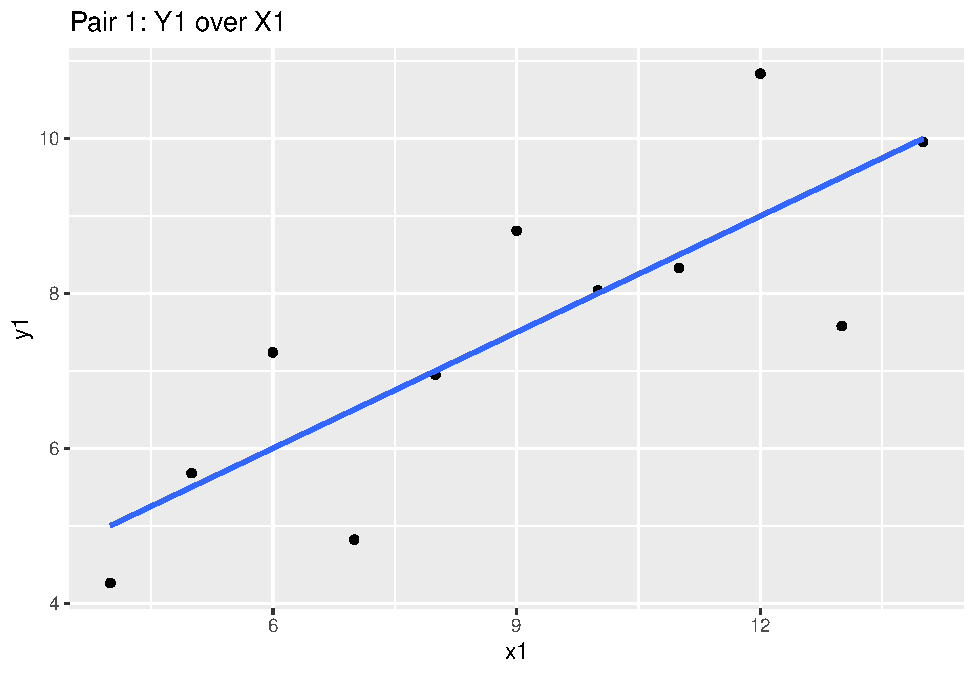
\includegraphics[width=0.5\linewidth]{Audit_Analytics_with-R_files/figure-latex/unnamed-chunk-95-1} 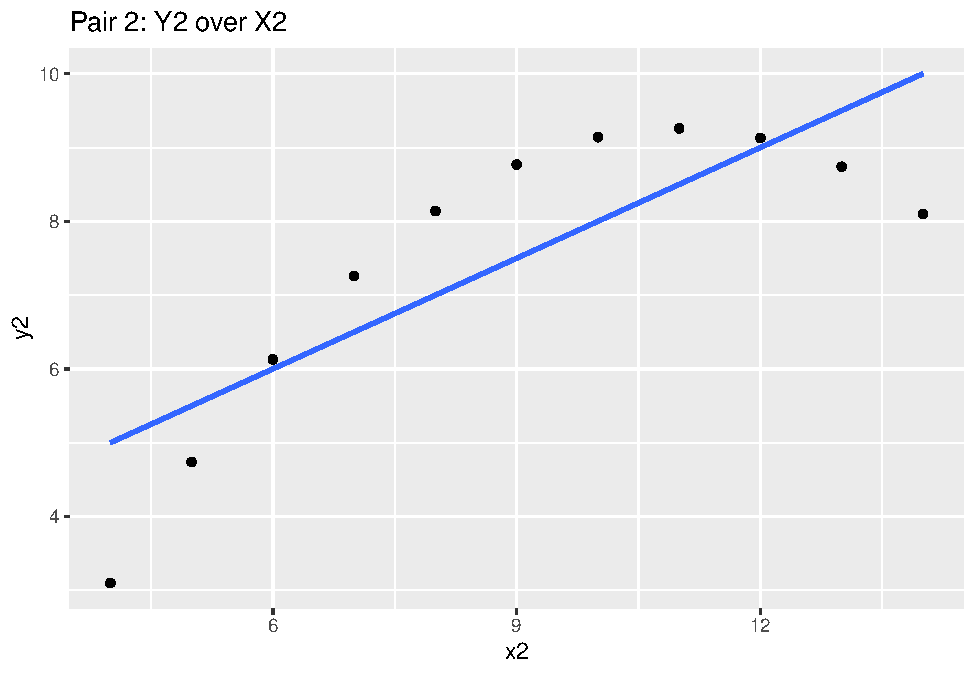
\includegraphics[width=0.5\linewidth]{Audit_Analytics_with-R_files/figure-latex/unnamed-chunk-95-2} 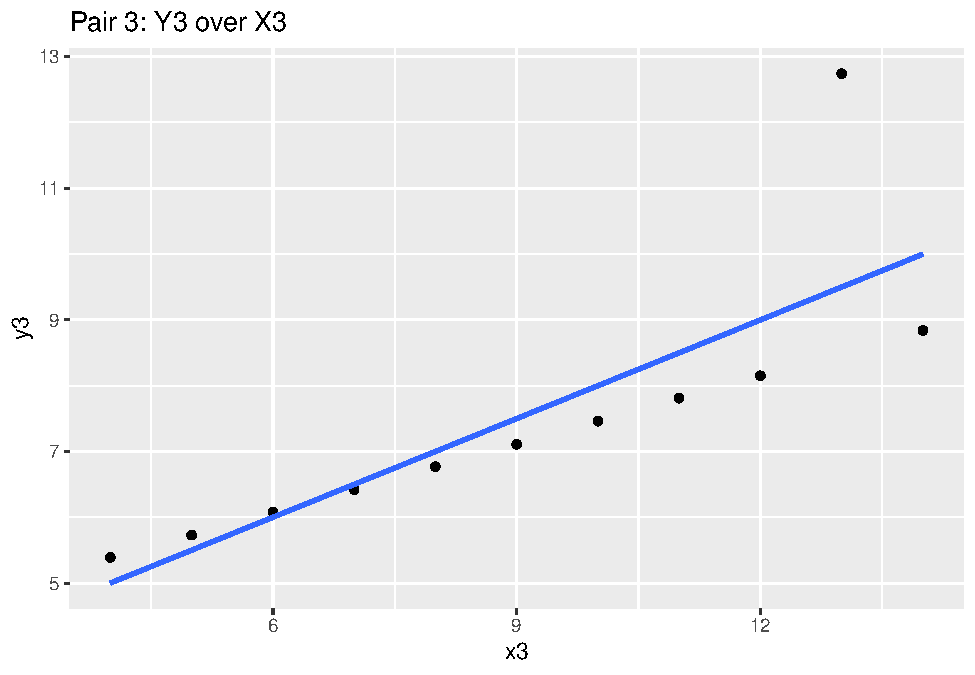
\includegraphics[width=0.5\linewidth]{Audit_Analytics_with-R_files/figure-latex/unnamed-chunk-95-3} 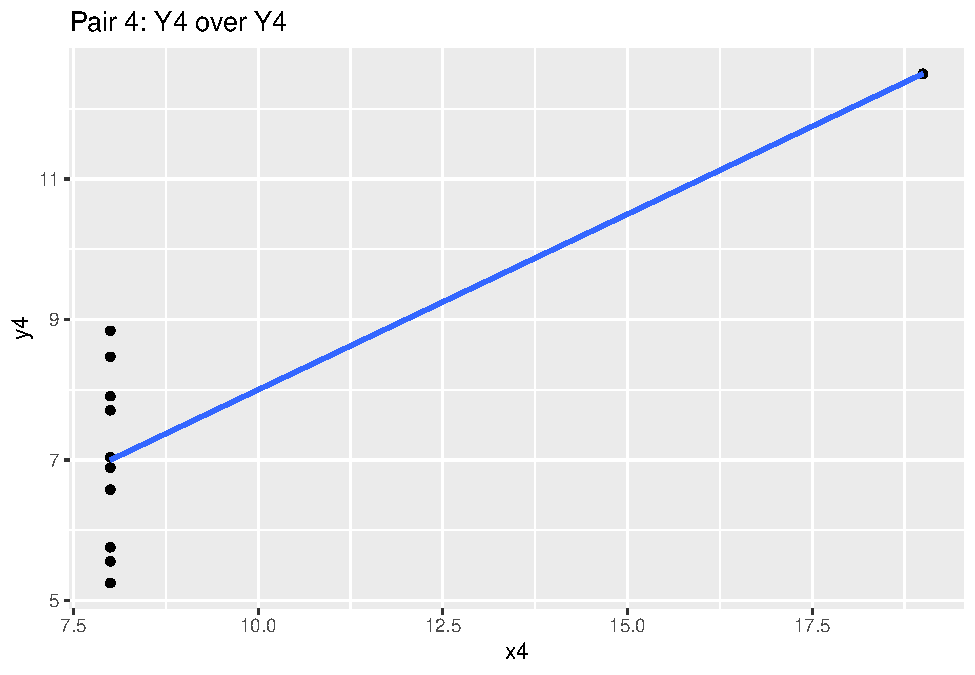
\includegraphics[width=0.5\linewidth]{Audit_Analytics_with-R_files/figure-latex/unnamed-chunk-95-4}

These four charts and scatterplots themselves are quite different! While the blue correlation line and the prior summary statistics are similar, the points all follow a different general path. Independently looking at the graphics for each one will give you different insight, and may influence your audit approach. Graphics matter a lot!

\hypertarget{data-visualization---how}{%
\section{Data Visualization - How}\label{data-visualization---how}}

\emph{ggplot2} is the package that many consider to be one of the differentiating strengths of the R universe. It is one of the most elegant methods of visualizing data, and will help you understand your audit subject.

Back to our materials analysis.

\begin{Shaded}
\begin{Highlighting}[]
\NormalTok{materials }\OperatorTok
\StringTok{  }\KeywordTok{arrange}\NormalTok{(gl_date) }\OperatorTok
\StringTok{  }\KeywordTok{head}\NormalTok{()}
\end{Highlighting}
\end{Shaded}

\begin{verbatim}
## # A tibble: 6 x 8
##   je_num amount gl_date    vendor_id account  invoice_date description paid_date
##    <int>  <dbl> <date>         <int> <chr>           <dbl> <chr>           <dbl>
## 1    373 13520. 2019-01-01      2612 exp_mat~        17887 Paper           17920
## 2    951 13486. 2019-01-01      2612 exp_mat~        17887 Paper           17920
## 3    961 16026. 2019-01-01      2726 exp_mat~        17890 Quality co~     17900
## 4     90  3777. 2019-01-02      2612 exp_mat~        17888 Face mask ~     17921
## 5    115 13402. 2019-01-02      2211 exp_mat~        17891 Packaging ~     17928
## 6    198  2431. 2019-01-02      2612 exp_mat~        17888 Face mask ~     17921
\end{verbatim}

Perhaps we want to start analyzing the change over time for the amount spent. The \texttt{gl\_date} is useful here, although there are many transactions that occur on the same date. We also have a \texttt{vendor\_id} as well, identifying the vendor that the transaction the invoice belongs to.

Generally we will want our time to be the x variable (the dependent variable), and the amount spent to be the y variable (the independent variable). We can insert the x and y into a ggplot function and generate the visualization we think may reveal useful infromation.

\begin{Shaded}
\begin{Highlighting}[]
\KeywordTok{ggplot}\NormalTok{(}\DataTypeTok{data =}\NormalTok{ materials, }\DataTypeTok{mapping =} \KeywordTok{aes}\NormalTok{(}\DataTypeTok{x =}\NormalTok{ gl_date, }\DataTypeTok{y =}\NormalTok{ amount)) }\OperatorTok{+}
\StringTok{  }\KeywordTok{geom_point}\NormalTok{()}
\end{Highlighting}
\end{Shaded}

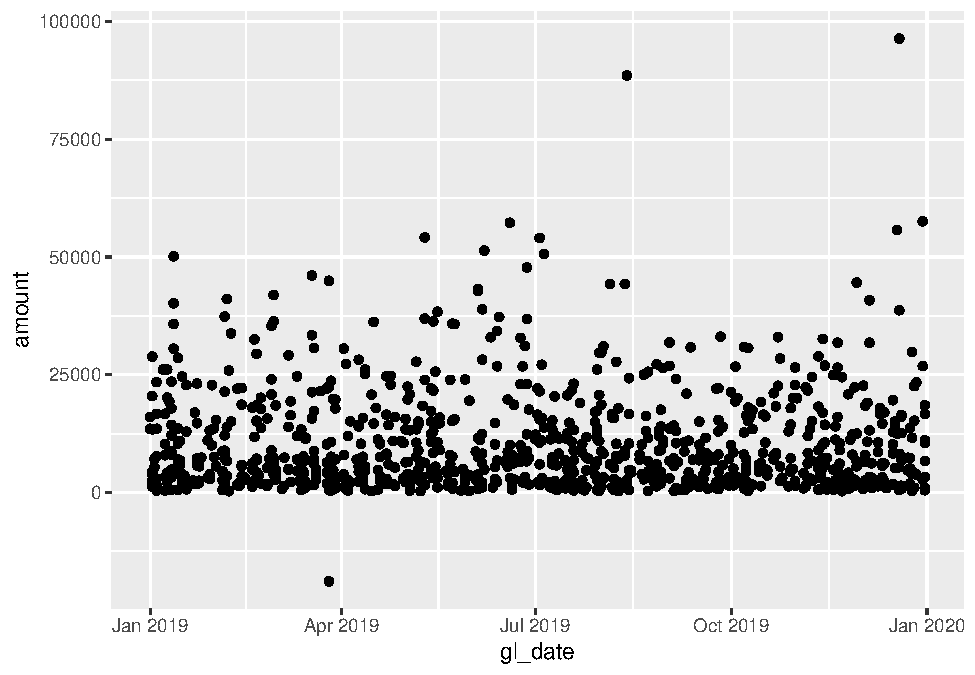
\includegraphics{Audit_Analytics_with-R_files/figure-latex/unnamed-chunk-97-1.pdf}

The foundations of any ggplot are essentially:

\begin{itemize}
\tightlist
\item
  \texttt{data} - The data frame you want to visualize,
\item
  \texttt{mapping} - The aesthetics, which dictate the x and y (generally for the rest of the ggplot), and
\item
  \texttt{geom\_*} - The visualization mechanism you want to apply to represent the data points.
\end{itemize}

When you specify a single \texttt{mapping} up front, it will be used for all the subsequent geoms called. You can also specify a mapping for each geom as well, which is useful for isolating points.

This foundations layer of \texttt{data}, \texttt{mapping} and \texttt{geom\_*} allows us to call different geoms and perspectives of looking at the data.

For example, histograms are useful to understand the shape of a dataset:

\begin{Shaded}
\begin{Highlighting}[]
\KeywordTok{ggplot}\NormalTok{(materials, }\KeywordTok{aes}\NormalTok{(}\DataTypeTok{x =}\NormalTok{ amount)) }\OperatorTok{+}\StringTok{ }\CommentTok{# data is the first default argument, and mapping is the second}
\StringTok{  }\KeywordTok{geom_histogram}\NormalTok{()}
\end{Highlighting}
\end{Shaded}

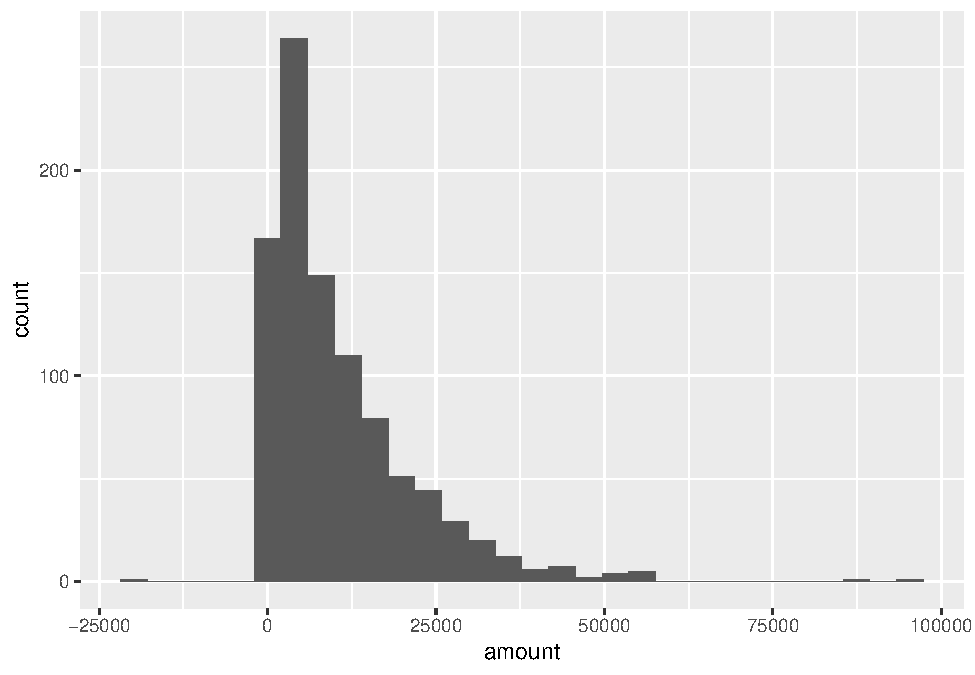
\includegraphics{Audit_Analytics_with-R_files/figure-latex/unnamed-chunk-98-1.pdf}

And boxplots are useful to understand the distribution of the data:

\begin{Shaded}
\begin{Highlighting}[]
\KeywordTok{ggplot}\NormalTok{(}\DataTypeTok{data =}\NormalTok{ materials, }\KeywordTok{aes}\NormalTok{(}\DataTypeTok{x =} \KeywordTok{as.factor}\NormalTok{(vendor_id), }\DataTypeTok{y =}\NormalTok{ amount)) }\OperatorTok{+}
\StringTok{  }\KeywordTok{geom_boxplot}\NormalTok{()}
\end{Highlighting}
\end{Shaded}

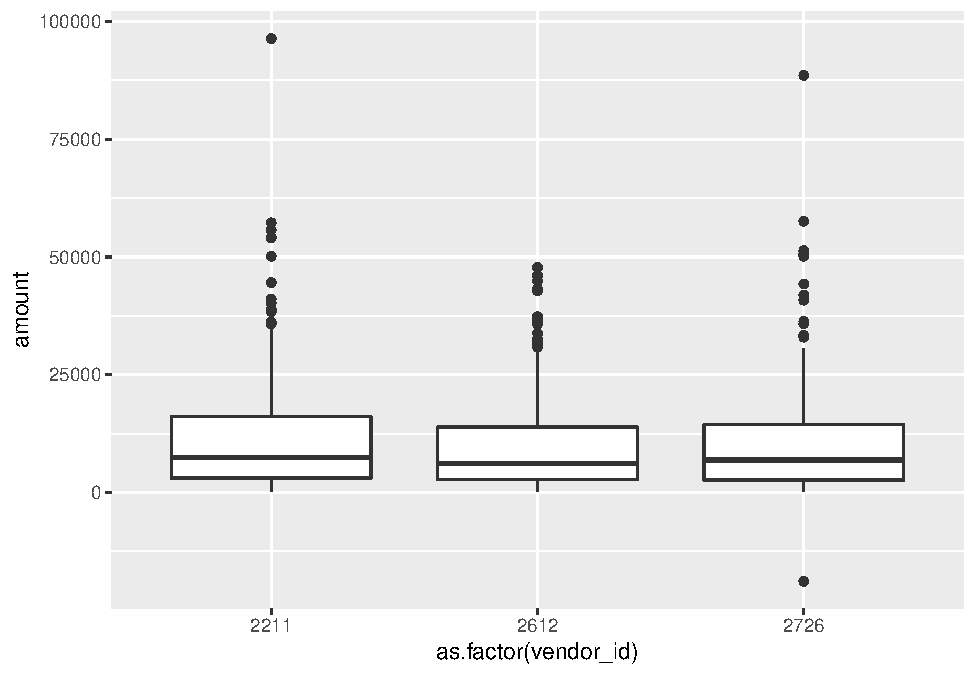
\includegraphics{Audit_Analytics_with-R_files/figure-latex/unnamed-chunk-99-1.pdf}

\hypertarget{time-series}{%
\subsection{Time-series}\label{time-series}}

As the gl table (and materials subset) is a time-series data, containing both the transaction date and amount, we may want to try plotting a line chart to see the movement of data over time.

\begin{Shaded}
\begin{Highlighting}[]
\KeywordTok{ggplot}\NormalTok{(}\DataTypeTok{data =}\NormalTok{ materials, }\KeywordTok{aes}\NormalTok{(}\DataTypeTok{x =}\NormalTok{ gl_date, }\DataTypeTok{y =}\NormalTok{ amount)) }\OperatorTok{+}
\StringTok{  }\KeywordTok{geom_line}\NormalTok{()}
\end{Highlighting}
\end{Shaded}

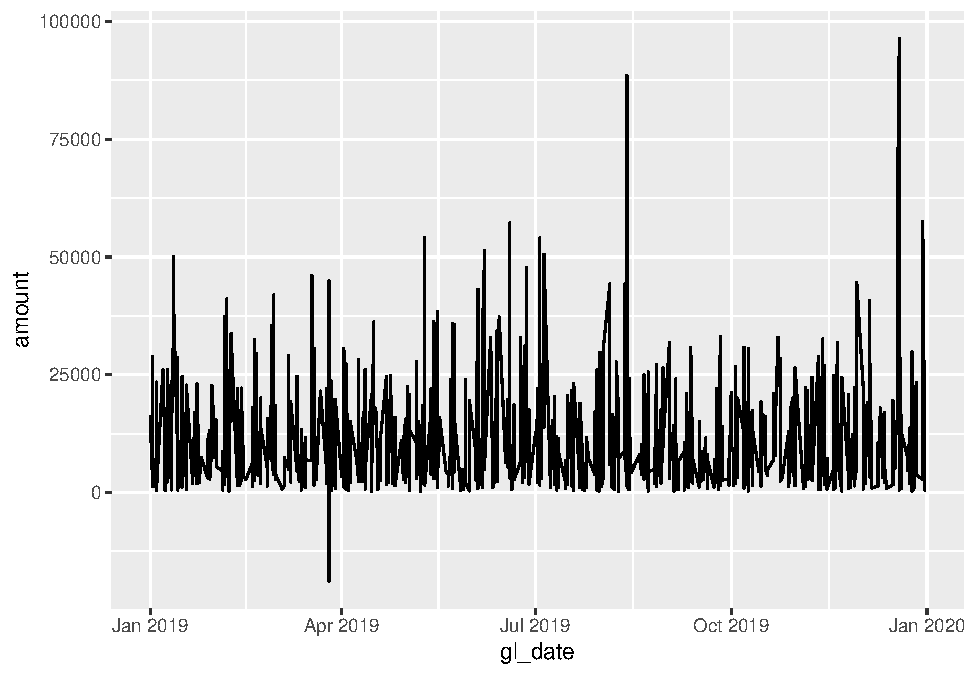
\includegraphics{Audit_Analytics_with-R_files/figure-latex/unnamed-chunk-100-1.pdf}

Since our time-series data has a relatively high resolution with detailed data, we may sometimes gain insight by aggregating data (by week, month, or even year). As of now, the data needs to be aggregated into a higher level time period.

\begin{Shaded}
\begin{Highlighting}[]
\NormalTok{monthly_mats <-}\StringTok{ }\NormalTok{materials }\OperatorTok
\StringTok{  }\KeywordTok{mutate}\NormalTok{(}\DataTypeTok{gl_month =} \KeywordTok{floor_date}\NormalTok{(gl_date, }\StringTok{'month'}\NormalTok{)) }\OperatorTok\StringTok{ }\CommentTok{# Rounds the date down to the first of the month}
\StringTok{  }\KeywordTok{group_by}\NormalTok{(gl_month) }\OperatorTok
\StringTok{  }\KeywordTok{summarize}\NormalTok{(}\DataTypeTok{amount =} \KeywordTok{sum}\NormalTok{(amount))}
\end{Highlighting}
\end{Shaded}

\begin{verbatim}
## `summarise()` ungrouping output (override with `.groups` argument)
\end{verbatim}

\begin{Shaded}
\begin{Highlighting}[]
\KeywordTok{head}\NormalTok{(monthly_mats)}
\end{Highlighting}
\end{Shaded}

\begin{verbatim}
## # A tibble: 6 x 2
##   gl_month     amount
##   <date>        <dbl>
## 1 2019-01-01 1021508.
## 2 2019-02-01  834766.
## 3 2019-03-01  746621.
## 4 2019-04-01  636011.
## 5 2019-05-01  953909.
## 6 2019-06-01  951240.
\end{verbatim}

Aggregating this same information by month may be more illustrative:

\begin{Shaded}
\begin{Highlighting}[]
\KeywordTok{ggplot}\NormalTok{(}\DataTypeTok{data =}\NormalTok{ monthly_mats, }\KeywordTok{aes}\NormalTok{(}\DataTypeTok{x =}\NormalTok{ gl_month, }\DataTypeTok{y =}\NormalTok{ amount)) }\OperatorTok{+}
\StringTok{  }\KeywordTok{geom_line}\NormalTok{()}
\end{Highlighting}
\end{Shaded}

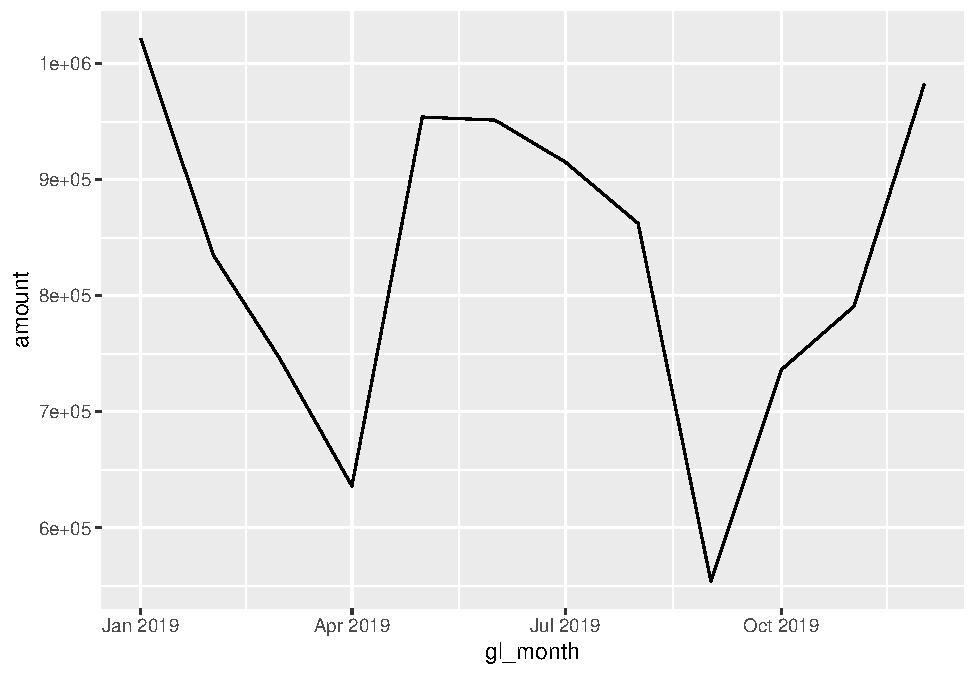
\includegraphics{Audit_Analytics_with-R_files/figure-latex/unnamed-chunk-102-1.pdf}

\hypertarget{facets}{%
\subsection{Facets}\label{facets}}

Another powerful feature of ggplot2 is facets - that is, the ability to show how different categories of the same data may look in the same dataset. In our GL dataset, we actually had multiple types of expenses:

\begin{Shaded}
\begin{Highlighting}[]
\KeywordTok{unique}\NormalTok{(gl}\OperatorTok{$}\NormalTok{account)}
\end{Highlighting}
\end{Shaded}

\begin{verbatim}
## [1] "exp_materials_6000"          "liab_accountspayable_2000"  
## [3] "exp_meals_7000"              "liab_creditcardpayable_2100"
## [5] "exp_consulting_6500"
\end{verbatim}

We can pull these specific expense accounts (starting with `exp\_'), and can choose how we want to plot them:

\begin{Shaded}
\begin{Highlighting}[]
\NormalTok{expense <-}\StringTok{ }\NormalTok{gl }\OperatorTok
\StringTok{  }\KeywordTok{filter}\NormalTok{(account }\OperatorTok\StringTok{ }\KeywordTok{c}\NormalTok{(}\StringTok{'exp_materials_6000'}\NormalTok{, }\StringTok{'exp_consulting_6500'}\NormalTok{, }\StringTok{'exp_meals_7000'}\NormalTok{)) }\OperatorTok
\StringTok{  }\KeywordTok{mutate}\NormalTok{(}\DataTypeTok{gl_date =} \KeywordTok{as_date}\NormalTok{(gl_date_char),}
         \DataTypeTok{gl_month =} \KeywordTok{floor_date}\NormalTok{(gl_date, }\StringTok{'month'}\NormalTok{)) }\OperatorTok\StringTok{ }
\StringTok{  }\KeywordTok{group_by}\NormalTok{(account, gl_month) }\OperatorTok\StringTok{ }\CommentTok{# Need to add a new layer of grouping to preserve the account}
\StringTok{  }\KeywordTok{summarize}\NormalTok{(}\DataTypeTok{amount =} \KeywordTok{sum}\NormalTok{(amount))}
\end{Highlighting}
\end{Shaded}

\begin{verbatim}
## `summarise()` regrouping output by 'account' (override with `.groups` argument)
\end{verbatim}

\begin{Shaded}
\begin{Highlighting}[]
\KeywordTok{ggplot}\NormalTok{(}\DataTypeTok{data =}\NormalTok{ expense, }\KeywordTok{aes}\NormalTok{(}\DataTypeTok{x =}\NormalTok{ gl_month, }\DataTypeTok{y =}\NormalTok{ amount, }\DataTypeTok{colour =}\NormalTok{ account)) }\OperatorTok{+}\StringTok{ }\CommentTok{# We can specify the colour now too, depending on the geom_*}
\StringTok{  }\KeywordTok{geom_line}\NormalTok{()}
\end{Highlighting}
\end{Shaded}

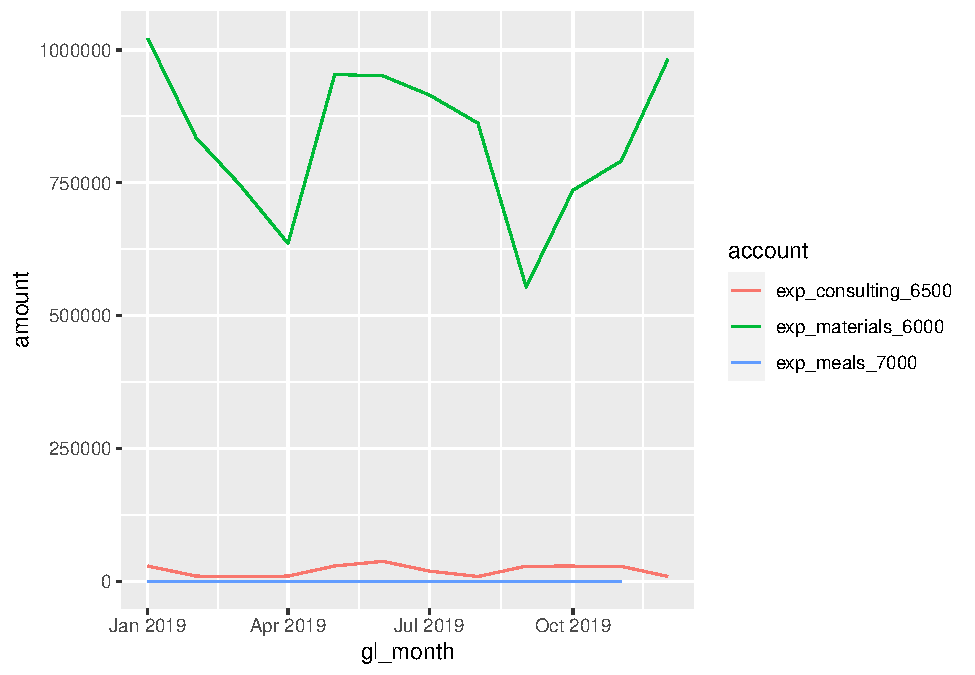
\includegraphics{Audit_Analytics_with-R_files/figure-latex/unnamed-chunk-104-1.pdf}

Instead of plotting them onto the same chart, we can \texttt{facet\_*} them:

\begin{Shaded}
\begin{Highlighting}[]
\KeywordTok{ggplot}\NormalTok{(}\DataTypeTok{data =}\NormalTok{ expense, }\KeywordTok{aes}\NormalTok{(}\DataTypeTok{x =}\NormalTok{ gl_month, }\DataTypeTok{y =}\NormalTok{ amount, }\DataTypeTok{colour =}\NormalTok{ account)) }\OperatorTok{+}
\StringTok{  }\KeywordTok{geom_line}\NormalTok{() }\OperatorTok{+}
\StringTok{  }\KeywordTok{facet_grid}\NormalTok{(. }\OperatorTok{~}\StringTok{ }\NormalTok{account) }\CommentTok{# Syntax for variable, either in the (row ~ column)... or both!}
\end{Highlighting}
\end{Shaded}

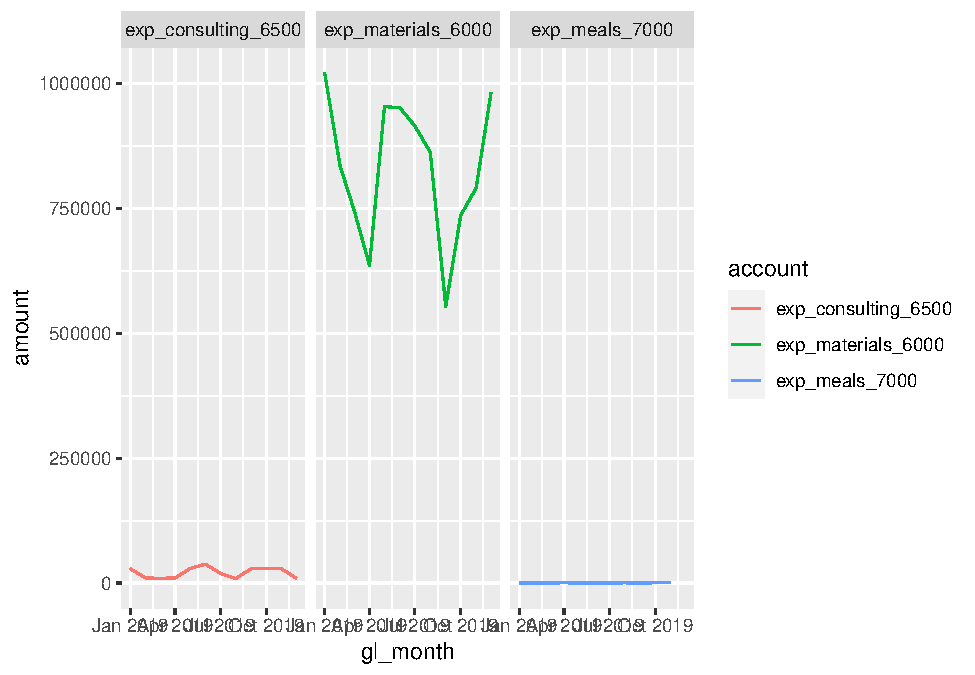
\includegraphics{Audit_Analytics_with-R_files/figure-latex/unnamed-chunk-105-1.pdf}

\hypertarget{test}{%
\chapter{Test}\label{test}}

Testing data is the act of isolating high-risk records that meet criteria. While generally the intent of data analytics within auditing is to gain 100\% population coverage and associated assurance, what will inevitably happen is that process deviations are revealed as items are detected. No process is bullet-proof and exception free, and therefore the auditor should have a founded idea of their level of risk tolerance prior to testing. Testing data will then help auditors articulate the nature of the exceptions and the overall risk level.

Auditors must recognize that not all tests (and lines that meet these tests) immediately ascertain that the control has failed or that something suspicious has occurred. Rather, it points to items that require further inspection and judgment. By iterating your workflow, you will be able to reduce the incidence of false positives and increase your detection rate, allowing you to focus on follow-up of higher-risk activity.

For this section we will use the company GL database.

\begin{Shaded}
\begin{Highlighting}[]
\KeywordTok{library}\NormalTok{(dplyr) }
\KeywordTok{library}\NormalTok{(tidyr) }
\KeywordTok{library}\NormalTok{(lubridate) }
\KeywordTok{library}\NormalTok{(DBI) }
\KeywordTok{library}\NormalTok{(ggplot2)}
\KeywordTok{library}\NormalTok{(gt) }\CommentTok{# Used for formatting outputs}
\KeywordTok{library}\NormalTok{(pryr) }\CommentTok{# Used to analyze encoding in text chapter}
\KeywordTok{library}\NormalTok{(stringi) }\CommentTok{# specialized string processing}

\KeywordTok{dir.create}\NormalTok{(}\StringTok{"data"}\NormalTok{, }\DataTypeTok{showWarnings =} \OtherTok{FALSE}\NormalTok{)}

\KeywordTok{download.file}\NormalTok{(}\DataTypeTok{url =} \StringTok{"https://github.com/jonlinca/auditanalytics/raw/master/data/rauditanalytics.sqlite"}\NormalTok{,}
             \DataTypeTok{destfile =} \StringTok{"data/rauditanalytics.sqlite"}\NormalTok{, }\DataTypeTok{mode =} \StringTok{"wb"}\NormalTok{)}

\NormalTok{con <-}\StringTok{ }\KeywordTok{dbConnect}\NormalTok{(RSQLite}\OperatorTok{::}\KeywordTok{SQLite}\NormalTok{(), }\StringTok{"data/rauditanalytics.sqlite"}\NormalTok{)}

\NormalTok{gl <-}\StringTok{ }\KeywordTok{tbl}\NormalTok{(con, }\StringTok{'gl'}\NormalTok{) }\OperatorTok
\StringTok{  }\KeywordTok{collect}\NormalTok{() }\OperatorTok
\StringTok{  }\KeywordTok{mutate}\NormalTok{(}\DataTypeTok{gl_date =} \KeywordTok{as_date}\NormalTok{(gl_date, }\DataTypeTok{origin =} \StringTok{'1970-01-01'}\NormalTok{),}
         \DataTypeTok{paid_date =} \KeywordTok{as_date}\NormalTok{(paid_date, }\DataTypeTok{origin =} \StringTok{'1970-01-01'}\NormalTok{),}
         \DataTypeTok{invoice_date =} \KeywordTok{as_date}\NormalTok{(invoice_date, }\DataTypeTok{origin =} \StringTok{'1970-01-01'}\NormalTok{)) }\OperatorTok
\StringTok{  }\KeywordTok{select}\NormalTok{(}\OperatorTok{-}\NormalTok{gl_date_char)}

\KeywordTok{dbDisconnect}\NormalTok{(con)}
\end{Highlighting}
\end{Shaded}

Our primary commands for this chapter will be \texttt{mutate()} and \texttt{filter()}. The \texttt{mutate()} command is useful for testing data, as it allows the auditor to add features and/or criteria to their testing. After records have been identified, \texttt{filter()} will extract the rows matching criteria.

While you may able to directly \texttt{filter()} rows based on criteria, you may find it more effective to instead create the new fields with \texttt{mutate()} that match the filter criteria. My style for documenting tests is to create any additional features needed, and then create a corresponding test column, with \texttt{t\_} as the prefix, and isolate for these invoices to perform inspection and follow-up. This has benefits in the long run, including:

\begin{itemize}
\tightlist
\item
  Keeping all the tests on the same record allows for an easier way to detect any row that met multiple criteria,
\item
  It is straightforward to extract the rows that meets a test, and
\item
  Each new column related to a specific a criteria is akin to feature engineering, enabling the reuse of the tests for machine learning applications.
\end{itemize}

There are practical reasons why you may need to create separate data frame objects, so do not prescribe exclusively to this method for extremely long or sophisticated steps. In cases when you have to perform multiple steps to get to your answer, it is advisable to bring the final result back into an overall reference table.

\hypertarget{amount-based-tests}{%
\section{Amount-based tests}\label{amount-based-tests}}

\hypertarget{above-threshold}{%
\subsection{Above threshold}\label{above-threshold}}

The most classical test is to test items that meet or exceed a material value.

\begin{Shaded}
\begin{Highlighting}[]
\NormalTok{gl }\OperatorTok
\StringTok{  }\KeywordTok{mutate}\NormalTok{(}\DataTypeTok{t_over_te =}\NormalTok{ amount }\OperatorTok{>=}\StringTok{ }\DecValTok{60000}\NormalTok{) }\OperatorTok
\StringTok{  }\KeywordTok{filter}\NormalTok{(t_over_te) }\OperatorTok
\StringTok{  }\KeywordTok{select}\NormalTok{(je_num, amount, }\KeywordTok{everything}\NormalTok{())}
\end{Highlighting}
\end{Shaded}

\begin{verbatim}
## # A tibble: 2 x 9
##   je_num amount gl_date    vendor_id account invoice_date description paid_date 
##    <int>  <dbl> <date>         <int> <chr>   <date>       <chr>       <date>    
## 1    140 96355. 2019-12-19      2211 exp_ma~ 2019-12-12   Packaging ~ 2020-01-18
## 2    693 88524. 2019-08-13      2726 exp_ma~ 2019-08-06   Quality co~ 2019-08-16
## # ... with 1 more variable: t_over_te <lgl>
\end{verbatim}

When performing amount or threshold testing, you may be more interested in the actual magnitude, and not necessarily the direction. This is especially true within accounting matters, where the implication of negative and positive amounts change depending on the transaction - i.e., a debit or a credit transaction, or affecting a balance sheet or income statement account can tell a very different story.

In these cases, you may want to consider using absolute values as the comparison. This allows you to capture the magnitude of the change:

\begin{Shaded}
\begin{Highlighting}[]
\NormalTok{gl }\OperatorTok
\StringTok{  }\KeywordTok{mutate}\NormalTok{(}\DataTypeTok{t_over_te =} \KeywordTok{abs}\NormalTok{(amount) }\OperatorTok{>=}\StringTok{ }\DecValTok{60000}\NormalTok{) }\OperatorTok
\StringTok{  }\KeywordTok{filter}\NormalTok{(t_over_te)}
\end{Highlighting}
\end{Shaded}

\begin{verbatim}
## # A tibble: 4 x 9
##   je_num  amount gl_date    vendor_id account invoice_date description
##    <int>   <dbl> <date>         <int> <chr>   <date>       <chr>      
## 1    140  96355. 2019-12-19      2211 exp_ma~ 2019-12-12   Packaging ~
## 2    140 -96355. 2019-12-19        NA liab_a~ 2019-12-12   Packaging ~
## 3    693  88524. 2019-08-13      2726 exp_ma~ 2019-08-06   Quality co~
## 4    693 -88524. 2019-08-13        NA liab_a~ 2019-08-06   Quality co~
## # ... with 2 more variables: paid_date <date>, t_over_te <lgl>
\end{verbatim}

\hypertarget{round-numbers}{%
\subsection{Round numbers}\label{round-numbers}}

In forensic accounting, auditors tend to take the position that transactions rarely end in whole dollars, especially if they end in multiples of 5, or even in multiples of tens.

Detection of these is contingent on the use of \texttt{\%\%}, better known as the modulo operator. It will calculate the remainder of a division calculation; dividing 1.50 by 1 will give you a remainder of 0.5.

\begin{Shaded}
\begin{Highlighting}[]
\FloatTok{1.50} \OperatorTok\StringTok{ }\DecValTok{1}
\end{Highlighting}
\end{Shaded}

\begin{verbatim}
## [1] 0.5
\end{verbatim}

This same approach can be used to detect if a transaction is round, i.e.~has no `cents' in it. How you decide to apply this can be useful in many cases. For example, finding a transaction that happens to be cleanly in the `thousands', perform the modulo by the corresponding amount and look for results where the remainder is 0.

\begin{Shaded}
\begin{Highlighting}[]
\DecValTok{15000} \OperatorTok\StringTok{ }\DecValTok{1000}
\end{Highlighting}
\end{Shaded}

\begin{verbatim}
## [1] 0
\end{verbatim}

Or even a round five number, which has its use cases when it comes to things like gift cards or tipping at restaurants:

\begin{Shaded}
\begin{Highlighting}[]
\DecValTok{25} \OperatorTok\StringTok{ }\DecValTok{5}
\end{Highlighting}
\end{Shaded}

\begin{verbatim}
## [1] 0
\end{verbatim}

When implementing as a test, I'd encourage creating multiple tests to see which test it matched, and then detect these variations together:

\begin{Shaded}
\begin{Highlighting}[]
\NormalTok{gl }\OperatorTok
\StringTok{  }\KeywordTok{mutate}\NormalTok{(}\DataTypeTok{t_round_5 =}\NormalTok{ amount }\OperatorTok\StringTok{ }\DecValTok{5} \OperatorTok{==}\StringTok{ }\DecValTok{0}\NormalTok{,}
         \DataTypeTok{t_round_10 =}\NormalTok{ amount }\OperatorTok\StringTok{ }\DecValTok{10} \OperatorTok{==}\StringTok{ }\DecValTok{0}\NormalTok{,}
         \DataTypeTok{t_round_100 =}\NormalTok{ amount }\OperatorTok\StringTok{ }\DecValTok{100} \OperatorTok{==}\StringTok{ }\DecValTok{0}\NormalTok{,}
         \DataTypeTok{t_round_1000 =}\NormalTok{ amount }\OperatorTok\StringTok{ }\DecValTok{1000} \OperatorTok{==}\StringTok{ }\DecValTok{0}\NormalTok{) }\OperatorTok
\StringTok{  }\KeywordTok{filter_at}\NormalTok{(}\KeywordTok{vars}\NormalTok{(}\KeywordTok{starts_with}\NormalTok{(}\StringTok{"t_round"}\NormalTok{)), }\KeywordTok{any_vars}\NormalTok{(.)) }\OperatorTok
\StringTok{  }\KeywordTok{select}\NormalTok{(je_num, amount, }\KeywordTok{starts_with}\NormalTok{(}\StringTok{"t_round"}\NormalTok{))}
\end{Highlighting}
\end{Shaded}

\begin{verbatim}
## # A tibble: 2 x 6
##   je_num amount t_round_5 t_round_10 t_round_100 t_round_1000
##    <int>  <dbl> <lgl>     <lgl>      <lgl>       <lgl>       
## 1    621  12800 TRUE      TRUE       TRUE        FALSE       
## 2    621 -12800 TRUE      TRUE       TRUE        FALSE
\end{verbatim}

\hypertarget{date-based-tests}{%
\section{Date-based tests}\label{date-based-tests}}

\hypertarget{weekend-testing}{%
\subsection{Weekend testing}\label{weekend-testing}}

As a typical office business (along with office activities) generally happen on the weekday - that is, Monday through Friday. We may be interested in selecting journal entries from a sample of activities that occurred on the weekend. To test this, we can use the \textbf{lubridate} package to determine what day of week our entry falls upon:

\begin{Shaded}
\begin{Highlighting}[]
\NormalTok{gl <-}\StringTok{ }\NormalTok{gl }\OperatorTok
\StringTok{  }\KeywordTok{mutate}\NormalTok{(}\DataTypeTok{day_of_week =} \KeywordTok{wday}\NormalTok{(gl_date, }\DataTypeTok{label =} \OtherTok{TRUE}\NormalTok{),  }\CommentTok{# Label is useful if you tend to forget what each number means}
         \DataTypeTok{t_weekend =}\NormalTok{ day_of_week }\OperatorTok\StringTok{ }\KeywordTok{c}\NormalTok{(}\StringTok{'Sat'}\NormalTok{, }\StringTok{'Sun'}\NormalTok{))}

\NormalTok{gl }\OperatorTok
\StringTok{  }\KeywordTok{filter}\NormalTok{(t_weekend) }\OperatorTok
\StringTok{  }\KeywordTok{head}\NormalTok{()}
\end{Highlighting}
\end{Shaded}

\begin{verbatim}
## # A tibble: 6 x 10
##   je_num  amount gl_date    vendor_id account invoice_date description
##    <int>   <dbl> <date>         <int> <chr>   <date>       <chr>      
## 1     54  35758. 2019-01-12      2612 exp_ma~ 2019-01-02   Face mask ~
## 2     54 -35758. 2019-01-12        NA liab_a~ 2019-01-02   Face mask ~
## 3    102  50135. 2019-01-12      2726 exp_ma~ 2019-01-05   Medical gr~
## 4    102 -50135. 2019-01-12        NA liab_a~ 2019-01-05   Medical gr~
## 5    223  50128. 2019-01-12      2211 exp_ma~ 2019-01-05   Packaging ~
## 6    223 -50128. 2019-01-12        NA liab_a~ 2019-01-05   Packaging ~
## # ... with 3 more variables: paid_date <date>, day_of_week <ord>,
## #   t_weekend <lgl>
\end{verbatim}

\hypertarget{cutoff-testing}{%
\subsection{Cutoff testing}\label{cutoff-testing}}

When transactions are near the end of the month (or the end of the year), cutoff testing helps establish that the transactions were recorded within the correct time period. Testing these may require selecting invoices close to month end.

Similar to how we calculate the period using \texttt{floor\_date()}, we can take any date and transform it with \texttt{ceiling\_date()} which will calculate the last date of the month. Then we can test to see if a date falls within the range as needed.

\begin{Shaded}
\begin{Highlighting}[]
\NormalTok{gl }\OperatorTok
\StringTok{  }\KeywordTok{mutate}\NormalTok{(}\DataTypeTok{end_of_month =} \KeywordTok{ceiling_date}\NormalTok{(gl_date, }\DataTypeTok{unit =} \StringTok{'month'}\NormalTok{)) }\OperatorTok
\StringTok{  }\KeywordTok{select}\NormalTok{(gl_date, end_of_month) }\OperatorTok
\StringTok{  }\KeywordTok{head}\NormalTok{()}
\end{Highlighting}
\end{Shaded}

\begin{verbatim}
## # A tibble: 6 x 2
##   gl_date    end_of_month
##   <date>     <date>      
## 1 2019-12-02 2020-01-01  
## 2 2019-12-02 2020-01-01  
## 3 2019-11-28 2019-12-01  
## 4 2019-11-28 2019-12-01  
## 5 2019-04-09 2019-05-01  
## 6 2019-04-09 2019-05-01
\end{verbatim}

This is close to our desired result, but all these dates are representative of the beginning of the following month. To transform dates, simply use the unit as desired and treat it like a \protect\hyperlink{differences-between-time}{math calculation}. As all these dates are one day ahead, a \texttt{days} difference calculation will suffice:

\begin{Shaded}
\begin{Highlighting}[]
\NormalTok{gl <-}\StringTok{ }\NormalTok{gl }\OperatorTok
\StringTok{  }\KeywordTok{mutate}\NormalTok{(}\DataTypeTok{end_of_month =} \KeywordTok{ceiling_date}\NormalTok{(gl_date, }\DataTypeTok{unit =} \StringTok{'month'}\NormalTok{) }\OperatorTok{-}\StringTok{ }\KeywordTok{days}\NormalTok{(}\DecValTok{1}\NormalTok{))}

\NormalTok{gl }\OperatorTok
\StringTok{  }\KeywordTok{select}\NormalTok{(gl_date, end_of_month) }\OperatorTok
\StringTok{  }\KeywordTok{head}\NormalTok{()}
\end{Highlighting}
\end{Shaded}

\begin{verbatim}
## # A tibble: 6 x 2
##   gl_date    end_of_month
##   <date>     <date>      
## 1 2019-12-02 2019-12-31  
## 2 2019-12-02 2019-12-31  
## 3 2019-11-28 2019-11-30  
## 4 2019-11-28 2019-11-30  
## 5 2019-04-09 2019-04-30  
## 6 2019-04-09 2019-04-30
\end{verbatim}

And to detect which lines are close to month end, simply calculate the difference between the end of month and the original date, keeping only dates very close to the end of the month:

\begin{Shaded}
\begin{Highlighting}[]
\NormalTok{gl }\OperatorTok
\StringTok{  }\KeywordTok{mutate}\NormalTok{(}\DataTypeTok{t_cutoff =}\NormalTok{ (end_of_month }\OperatorTok{-}\StringTok{ }\NormalTok{gl_date) }\OperatorTok{<=}\StringTok{ }\DecValTok{1}\NormalTok{) }\OperatorTok\StringTok{ }\CommentTok{# Find entries on or one day prior to month end}
\StringTok{  }\KeywordTok{filter}\NormalTok{(t_cutoff) }\OperatorTok
\StringTok{  }\KeywordTok{select}\NormalTok{(je_num, gl_date, t_cutoff, }\KeywordTok{everything}\NormalTok{())}
\end{Highlighting}
\end{Shaded}

\begin{verbatim}
## # A tibble: 136 x 12
##    je_num gl_date    t_cutoff  amount vendor_id account invoice_date description
##     <int> <date>     <lgl>      <dbl>     <int> <chr>   <date>       <chr>      
##  1      4 2019-10-30 TRUE      20037.      2612 exp_ma~ 2019-10-20   Paper      
##  2      4 2019-10-30 TRUE     -20037.        NA liab_a~ 2019-10-20   Paper      
##  3      6 2019-01-31 TRUE      13603.      2726 exp_ma~ 2019-01-24   Medical gr~
##  4      6 2019-01-31 TRUE     -13603.        NA liab_a~ 2019-01-24   Medical gr~
##  5     11 2019-07-30 TRUE       3000.      2612 exp_ma~ 2019-07-20   Paper      
##  6     11 2019-07-30 TRUE      -3000.        NA liab_a~ 2019-07-20   Paper      
##  7     31 2019-04-29 TRUE       9931.      2211 exp_co~ 2019-04-14   Advisory s~
##  8     31 2019-04-29 TRUE      -9931.        NA liab_a~ 2019-04-14   Advisory s~
##  9     44 2019-02-28 TRUE       3838.      2211 exp_ma~ 2019-02-21   Packaging ~
## 10     44 2019-02-28 TRUE      -3838.        NA liab_a~ 2019-02-21   Packaging ~
## # ... with 126 more rows, and 4 more variables: paid_date <date>,
## #   day_of_week <ord>, t_weekend <lgl>, end_of_month <date>
\end{verbatim}

\hypertarget{age}{%
\subsection{Age}\label{age}}

Aging invoices is generally a system-ran report out of the accounting system. Independently testing these reports is one of the strongest forms of assurance, which requires an understanding of the underlying data, including calculation accuracy and completeness.

At its core, an aging calculation is the comparison of one date to another certain date, and then aggregating the total amount by buckets indicating a range of days. However, it gets complicated rather quick because of how different systems implement aging:

\begin{itemize}
\tightlist
\item
  Which dates are being compared - invoice dates, entry dates, paid dates and/or due dates?
\item
  Speaking of due dates, are you able to calculate a due date on a per-vendor (or even, per invoice) basis?
\item
  Are you able to run a report `as-of'? The as-of date is intended to help understand the outstanding balances at a specific point of time. Some accounting systems have insufficient information captured, meaning a backdated entered invoice (perhaps to a prior period) may affect the accuracy of a previous report.
\end{itemize}

We will initially filter our data and only keep valid invoices, by filtering on records that are related to materials:

\begin{Shaded}
\begin{Highlighting}[]
\NormalTok{gl }\OperatorTok
\StringTok{  }\KeywordTok{filter}\NormalTok{(account }\OperatorTok{==}\StringTok{ 'exp_materials_6000'}\NormalTok{) }\OperatorTok\StringTok{ }\CommentTok{# In scope invoices for aging}
\StringTok{  }\KeywordTok{select}\NormalTok{(je_num, vendor_id, gl_date, invoice_date, paid_date)}
\end{Highlighting}
\end{Shaded}

\begin{verbatim}
## # A tibble: 952 x 5
##    je_num vendor_id gl_date    invoice_date paid_date 
##     <int>     <int> <date>     <date>       <date>    
##  1      1      2211 2019-12-02 2019-11-25   2020-01-01
##  2      2      2612 2019-11-28 2019-11-18   2019-12-21
##  3      3      2612 2019-04-09 2019-03-30   2019-05-02
##  4      4      2612 2019-10-30 2019-10-20   2019-11-22
##  5      5      2612 2019-06-04 2019-05-25   2019-06-27
##  6      6      2726 2019-01-31 2019-01-24   2019-02-03
##  7      7      2726 2019-10-21 2019-10-14   2019-10-24
##  8      8      2211 2019-04-24 2019-04-17   2019-05-24
##  9      9      2726 2019-07-10 2019-07-03   2019-07-13
## 10     10      2211 2019-06-13 2019-06-06   2019-07-13
## # ... with 942 more rows
\end{verbatim}

In our GL data set, we have captured invoices (denoted as transactions against expense accounts), as well as the GL date (the day the company received the invoice), the invoice date as written by the supplier, and the date the invoice was paid.

With a better understanding of the dates, we can now focus on reproducing an accurate report:

\begin{itemize}
\tightlist
\item
  An invoice was recognized in our system as per the \texttt{gl\_date},
\item
  An invoice was considered fully paid as of the \texttt{paid\_date}, and
\item
  The definition of age in our system is based off the \texttt{invoice\_date} and an user-chosen `as-of' date.
\end{itemize}

We will use August 1, 2019 as our as-of date, and only include invoices that were recognized on or prior to then.

\begin{Shaded}
\begin{Highlighting}[]
\NormalTok{as_of_date <-}\StringTok{ }\KeywordTok{as.Date}\NormalTok{(}\StringTok{'2019-08-01'}\NormalTok{)}

\NormalTok{gl }\OperatorTok
\StringTok{  }\KeywordTok{filter}\NormalTok{(account }\OperatorTok{==}\StringTok{ 'exp_materials_6000'}\NormalTok{) }\OperatorTok\StringTok{ }\CommentTok{# In scope invoices for aging}
\StringTok{  }\KeywordTok{select}\NormalTok{(je_num, vendor_id, gl_date, invoice_date, paid_date) }\OperatorTok
\StringTok{  }\KeywordTok{filter}\NormalTok{(gl_date }\OperatorTok{<=}\StringTok{ }\NormalTok{as_of_date) }\CommentTok{# Only choose recognized invoices as of a date}
\end{Highlighting}
\end{Shaded}

\begin{verbatim}
## # A tibble: 571 x 5
##    je_num vendor_id gl_date    invoice_date paid_date 
##     <int>     <int> <date>     <date>       <date>    
##  1      3      2612 2019-04-09 2019-03-30   2019-05-02
##  2      5      2612 2019-06-04 2019-05-25   2019-06-27
##  3      6      2726 2019-01-31 2019-01-24   2019-02-03
##  4      8      2211 2019-04-24 2019-04-17   2019-05-24
##  5      9      2726 2019-07-10 2019-07-03   2019-07-13
##  6     10      2211 2019-06-13 2019-06-06   2019-07-13
##  7     11      2612 2019-07-30 2019-07-20   2019-08-22
##  8     12      2726 2019-06-19 2019-06-12   2019-06-22
##  9     16      2211 2019-01-18 2019-01-11   2019-02-17
## 10     17      2612 2019-02-05 2019-01-26   2019-02-28
## # ... with 561 more rows
\end{verbatim}

We can also remove any paid invoices too, as they're no longer aged as-of that date. Depending when you are running your report, an invoice may could either be paid or not paid yet.

\begin{Shaded}
\begin{Highlighting}[]
\NormalTok{gl }\OperatorTok
\StringTok{  }\KeywordTok{filter}\NormalTok{(account }\OperatorTok{==}\StringTok{ 'exp_materials_6000'}\NormalTok{) }\OperatorTok\StringTok{ }\CommentTok{# In scope invoices for aging}
\StringTok{  }\KeywordTok{select}\NormalTok{(je_num, vendor_id, gl_date, invoice_date, paid_date) }\OperatorTok
\StringTok{  }\KeywordTok{filter}\NormalTok{(gl_date }\OperatorTok{<=}\StringTok{ }\NormalTok{as_of_date) }\OperatorTok\StringTok{ }\CommentTok{# Only choose recognized invoices as of a date}
\StringTok{  }\KeywordTok{filter}\NormalTok{(paid_date }\OperatorTok{>=}\StringTok{ }\NormalTok{as_of_date }\OperatorTok{|}\StringTok{ }\KeywordTok{is.na}\NormalTok{(paid_date)) }\CommentTok{# Keep invoices that were not paid by the as-of date, or not paid at all yet}
\end{Highlighting}
\end{Shaded}

\begin{verbatim}
## # A tibble: 71 x 5
##    je_num vendor_id gl_date    invoice_date paid_date 
##     <int>     <int> <date>     <date>       <date>    
##  1     11      2612 2019-07-30 2019-07-20   2019-08-22
##  2     18      2612 2019-07-23 2019-07-13   2019-08-15
##  3     20      2211 2019-07-23 2019-07-16   2019-08-22
##  4     22      2612 2019-07-18 2019-07-08   2019-08-10
##  5     38      2211 2019-07-25 2019-07-18   2019-08-24
##  6     57      2211 2019-07-12 2019-07-05   2019-08-11
##  7     75      2211 2019-07-08 2019-07-01   2019-08-07
##  8     85      2612 2019-07-15 2019-07-05   2019-08-07
##  9     88      2612 2019-07-31 2019-07-21   2019-08-23
## 10     97      2612 2019-07-30 2019-07-20   2019-08-22
## # ... with 61 more rows
\end{verbatim}

Having isolated our invoices, we can now calculate the number of aged days:

\begin{Shaded}
\begin{Highlighting}[]
\NormalTok{gl }\OperatorTok
\StringTok{  }\KeywordTok{filter}\NormalTok{(account }\OperatorTok{==}\StringTok{ 'exp_materials_6000'}\NormalTok{) }\OperatorTok\StringTok{ }\CommentTok{# In scope invoices for aging}
\StringTok{  }\KeywordTok{filter}\NormalTok{(gl_date }\OperatorTok{<=}\StringTok{ }\NormalTok{as_of_date) }\OperatorTok\StringTok{ }\CommentTok{# Only choose recognized invoices as of a date}
\StringTok{  }\KeywordTok{filter}\NormalTok{(paid_date }\OperatorTok{>=}\StringTok{ }\NormalTok{as_of_date }\OperatorTok{|}\StringTok{ }\KeywordTok{is.na}\NormalTok{(paid_date)) }\OperatorTok\StringTok{ }\CommentTok{# Keep invoices that are not paid by the as-of date, or not paid at all yet}
\StringTok{  }\KeywordTok{mutate}\NormalTok{(}\DataTypeTok{aged_days =} \KeywordTok{as.numeric}\NormalTok{(as_of_date }\OperatorTok{-}\StringTok{ }\NormalTok{invoice_date)) }\OperatorTok
\StringTok{  }\KeywordTok{select}\NormalTok{(invoice_date, paid_date, aged_days)}
\end{Highlighting}
\end{Shaded}

\begin{verbatim}
## # A tibble: 71 x 3
##    invoice_date paid_date  aged_days
##    <date>       <date>         <dbl>
##  1 2019-07-20   2019-08-22        12
##  2 2019-07-13   2019-08-15        19
##  3 2019-07-16   2019-08-22        16
##  4 2019-07-08   2019-08-10        24
##  5 2019-07-18   2019-08-24        14
##  6 2019-07-05   2019-08-11        27
##  7 2019-07-01   2019-08-07        31
##  8 2019-07-05   2019-08-07        27
##  9 2019-07-21   2019-08-23        11
## 10 2019-07-20   2019-08-22        12
## # ... with 61 more rows
\end{verbatim}

Now the most complex part is making buckets for these ages. A rather brute force way is to create a field with the range it falls in, and then eventually pivoting on it:

\begin{Shaded}
\begin{Highlighting}[]
\NormalTok{aged_wip <-}\StringTok{ }\NormalTok{gl }\OperatorTok
\StringTok{  }\KeywordTok{filter}\NormalTok{(account }\OperatorTok{==}\StringTok{ 'exp_materials_6000'}\NormalTok{) }\OperatorTok\StringTok{ }\CommentTok{# In scope invoices for aging}
\StringTok{  }\KeywordTok{select}\NormalTok{(je_num, account, vendor_id, gl_date, invoice_date, paid_date) }\OperatorTok
\StringTok{  }\KeywordTok{filter}\NormalTok{(gl_date }\OperatorTok{<=}\StringTok{ }\NormalTok{as_of_date) }\OperatorTok\StringTok{ }\CommentTok{# Only choose recognized invoices as of a date}
\StringTok{  }\KeywordTok{filter}\NormalTok{(paid_date }\OperatorTok{>=}\StringTok{ }\NormalTok{as_of_date }\OperatorTok{|}\StringTok{ }\KeywordTok{is.na}\NormalTok{(paid_date)) }\OperatorTok\StringTok{ }\CommentTok{# Keep invoices that are not paid by the as-of date, or not paid at all yet}
\StringTok{  }\KeywordTok{mutate}\NormalTok{(}\DataTypeTok{aged_days =} \KeywordTok{as.numeric}\NormalTok{(as_of_date }\OperatorTok{-}\StringTok{ }\NormalTok{invoice_date)) }\OperatorTok
\StringTok{  }\KeywordTok{select}\NormalTok{(aged_days)}

\NormalTok{aged_wip }\OperatorTok
\StringTok{  }\KeywordTok{mutate}\NormalTok{(}\DataTypeTok{aging_bucket =} \KeywordTok{case_when}\NormalTok{(}
\NormalTok{    aged_days }\OperatorTok{<}\StringTok{ }\DecValTok{15} \OperatorTok{~}\StringTok{ "Current"}\NormalTok{,}
\NormalTok{    aged_days }\OperatorTok{<}\StringTok{ }\DecValTok{30} \OperatorTok{~}\StringTok{ "15 - 30"}\NormalTok{,}
\NormalTok{    aged_days }\OperatorTok{<}\StringTok{ }\DecValTok{90} \OperatorTok{~}\StringTok{ "30 - 59"}\NormalTok{,}
    \OtherTok{TRUE} \OperatorTok{~}\StringTok{ "60+"}
\NormalTok{  ))}
\end{Highlighting}
\end{Shaded}

\begin{verbatim}
## # A tibble: 71 x 2
##    aged_days aging_bucket
##        <dbl> <chr>       
##  1        12 Current     
##  2        19 15 - 30     
##  3        16 15 - 30     
##  4        24 15 - 30     
##  5        14 Current     
##  6        27 15 - 30     
##  7        31 30 - 59     
##  8        27 15 - 30     
##  9        11 Current     
## 10        12 Current     
## # ... with 61 more rows
\end{verbatim}

Another useful method is to use the \texttt{cut()} function, which will take the intervals you specify (aged days) and place each row into the category. The labels look a bit different - inclusive boundaries are \texttt{(} while exclusive boundaries are \texttt{{]}}:

\begin{Shaded}
\begin{Highlighting}[]
\NormalTok{aged_wip }\OperatorTok
\StringTok{  }\KeywordTok{mutate}\NormalTok{(}\DataTypeTok{aging_bucket =} \KeywordTok{cut}\NormalTok{(aged_wip}\OperatorTok{$}\NormalTok{aged_days, }\DataTypeTok{breaks =} \KeywordTok{c}\NormalTok{(}\DecValTok{0}\NormalTok{, }\DecValTok{15}\NormalTok{, }\DecValTok{30}\NormalTok{, }\DecValTok{60}\NormalTok{, }\OtherTok{Inf}\NormalTok{)))}
\end{Highlighting}
\end{Shaded}

\begin{verbatim}
## # A tibble: 71 x 2
##    aged_days aging_bucket
##        <dbl> <fct>       
##  1        12 (0,15]      
##  2        19 (15,30]     
##  3        16 (15,30]     
##  4        24 (15,30]     
##  5        14 (0,15]      
##  6        27 (15,30]     
##  7        31 (30,60]     
##  8        27 (15,30]     
##  9        11 (0,15]      
## 10        12 (0,15]      
## # ... with 61 more rows
\end{verbatim}

You can choose which approach best fits your style. With all the pieces, we can now create the aging report, aggregated by vendor. First, lets only keep the variables we want to pivot:

\begin{Shaded}
\begin{Highlighting}[]
\NormalTok{aged <-}\StringTok{ }\NormalTok{gl }\OperatorTok
\StringTok{  }\KeywordTok{filter}\NormalTok{(account }\OperatorTok{==}\StringTok{ 'exp_materials_6000'}\NormalTok{) }\OperatorTok\StringTok{ }\CommentTok{# In scope invoices for aging}
\StringTok{  }\KeywordTok{filter}\NormalTok{(gl_date }\OperatorTok{<=}\StringTok{ }\NormalTok{as_of_date) }\OperatorTok\StringTok{ }\CommentTok{# Only choose recognized invoices as of a date}
\StringTok{  }\KeywordTok{filter}\NormalTok{(paid_date }\OperatorTok{>=}\StringTok{ }\NormalTok{as_of_date }\OperatorTok{|}\StringTok{ }\KeywordTok{is.na}\NormalTok{(paid_date)) }\OperatorTok\StringTok{ }\CommentTok{# Keep invoices that are not paid by the as-of date, or not paid at all yet}
\StringTok{  }\KeywordTok{mutate}\NormalTok{(}\DataTypeTok{aged_days =} \KeywordTok{as.numeric}\NormalTok{(as_of_date }\OperatorTok{-}\StringTok{ }\NormalTok{invoice_date)) }\OperatorTok
\StringTok{  }\KeywordTok{mutate}\NormalTok{(}\DataTypeTok{aging_bucket =} \KeywordTok{case_when}\NormalTok{(}
\NormalTok{    aged_days }\OperatorTok{<}\StringTok{ }\DecValTok{15} \OperatorTok{~}\StringTok{ "Current"}\NormalTok{,}
\NormalTok{    aged_days }\OperatorTok{<}\StringTok{ }\DecValTok{30} \OperatorTok{~}\StringTok{ "15 - 30"}\NormalTok{,}
\NormalTok{    aged_days }\OperatorTok{<}\StringTok{ }\DecValTok{90} \OperatorTok{~}\StringTok{ "30 - 59"}\NormalTok{,}
    \OtherTok{TRUE} \OperatorTok{~}\StringTok{ "60+"}
\NormalTok{  )) }\OperatorTok
\StringTok{  }\KeywordTok{select}\NormalTok{(vendor_id, amount, aging_bucket)}

\KeywordTok{print}\NormalTok{(aged)}
\end{Highlighting}
\end{Shaded}

\begin{verbatim}
## # A tibble: 71 x 3
##    vendor_id amount aging_bucket
##        <int>  <dbl> <chr>       
##  1      2612  3000. Current     
##  2      2612  8436. 15 - 30     
##  3      2211   725. 15 - 30     
##  4      2612  5037. 15 - 30     
##  5      2211  7412. Current     
##  6      2211 11461. 15 - 30     
##  7      2211  2206. 30 - 59     
##  8      2612  2491. 15 - 30     
##  9      2612   294. Current     
## 10      2612 13593. Current     
## # ... with 61 more rows
\end{verbatim}

Since our typical aging report has vendors along the left (the unique identifier for \texttt{id\_cols} argument), aging buckets along the top (the names we want to spread across with \texttt{names\_from}) and the amount is a summation of the valid values (\texttt{values\_from} and also \texttt{values\_fn}), we can use \texttt{pivot\_wider()} to recreate our report:

\begin{Shaded}
\begin{Highlighting}[]
\NormalTok{aged }\OperatorTok
\StringTok{  }\KeywordTok{pivot_wider}\NormalTok{(}\DataTypeTok{id_cols =}\NormalTok{ vendor_id, }\DataTypeTok{names_from =}\NormalTok{ aging_bucket, }\DataTypeTok{values_from =}\NormalTok{ amount, }\DataTypeTok{values_fn =}\NormalTok{ sum)}
\end{Highlighting}
\end{Shaded}

\begin{verbatim}
## # A tibble: 3 x 4
##   vendor_id Current `15 - 30` `30 - 59`
##       <int>   <dbl>     <dbl>     <dbl>
## 1      2612  58163.    57468.    41684.
## 2      2211 120974.   114429.   136315.
## 3      2726 105586.       NA        NA
\end{verbatim}

\hypertarget{basic-statistical-tests}{%
\section{Basic Statistical tests}\label{basic-statistical-tests}}

In the \protect\hyperlink{explore-stats}{exploration of data}, we highlighted that exploring your data using various statistical functions are useful for helping understand the shape of your data. After doing so, you can then apply statistical methods directly in your testing to help select samples.

\hypertarget{outliers-based-on-amount}{%
\subsection{Outliers based on amount}\label{outliers-based-on-amount}}

\begin{quote}
An outlier is an observation that lies an abnormal distance from other values in a random sample from a population. In a sense, this definition leaves it up to the analyst (or a consensus process) to decide what will be considered abnormal. Before abnormal observations can be singled out, it is necessary to characterize normal observations. (\emph{NIST/Sematech E-Handbook of Statistical Methods}, \protect\hyperlink{ref-outliers}{n.d.})
\end{quote}

Our general approach to using statistical tests is to bring attention to ``abnormal'' entries in our data. Abnormal may be different depending on the situation, but items that stand apart from the rest are of audit interest.

Outliers are very specific to the dataset we are analyzing, and are highly dependent on the nature and structure of the work we have.

The most basic detection of extreme outliers can be done on an amount, looking for material transactions, by using the quantiles and IQRs. Quantiles indicate the thresholds where amounts may be in the bottom 25\% or above the top 75\% of data points. The IQR is defined as the difference between the upper 75\% quantile and lower 25\% quantile (i.e.~the 3rd quartile and 1st quartile).

The extreme outlier test is defined as points less than the 25\% quantile minus 1.5 * inter quartile range (IQR), or above the 75\% quantile plus 1.5 * IQR.

In this case, we want to detect items greater than the extreme upper outlier:

\begin{Shaded}
\begin{Highlighting}[]
\CommentTok{# Detect amounts in the top 25% of transactions}
\NormalTok{top_}\DecValTok{75}\NormalTok{ <-}\StringTok{ }\KeywordTok{quantile}\NormalTok{(}\KeywordTok{abs}\NormalTok{(gl}\OperatorTok{$}\NormalTok{amount))[}\DecValTok{4}\NormalTok{] }\CommentTok{# This is the 3st quartile, or the 75% quantile}
\NormalTok{iqr <-}\StringTok{ }\KeywordTok{IQR}\NormalTok{(}\KeywordTok{abs}\NormalTok{(gl}\OperatorTok{$}\NormalTok{amount))}
\NormalTok{upper_extreme_outlier <-}\StringTok{ }\NormalTok{top_}\DecValTok{75} \OperatorTok{+}\StringTok{ }\NormalTok{iqr }\OperatorTok{*}\StringTok{ }\FloatTok{1.5}

\KeywordTok{print}\NormalTok{(}\KeywordTok{paste0}\NormalTok{(}\StringTok{"The upper_extreme_outlier is $"}\NormalTok{, upper_extreme_outlier))}
\end{Highlighting}
\end{Shaded}

\begin{verbatim}
## [1] "The upper_extreme_outlier is $31929.19125"
\end{verbatim}

\begin{Shaded}
\begin{Highlighting}[]
\NormalTok{gl }\OperatorTok
\StringTok{  }\NormalTok{dplyr}\OperatorTok{::}\KeywordTok{filter}\NormalTok{(amount }\OperatorTok{>}\StringTok{ }\NormalTok{upper_extreme_outlier) }\OperatorTok
\StringTok{  }\KeywordTok{select}\NormalTok{(je_num, amount, account, description) }\OperatorTok
\StringTok{  }\KeywordTok{arrange}\NormalTok{(description)}
\end{Highlighting}
\end{Shaded}

\begin{verbatim}
## # A tibble: 46 x 4
##    je_num amount account            description            
##     <int>  <dbl> <chr>              <chr>                  
##  1      5 43140. exp_materials_6000 Blue dye               
##  2    430 37341. exp_materials_6000 Blue dye               
##  3    825 36918. exp_materials_6000 Blue dye               
##  4     70 32584. exp_materials_6000 Fabric cutting machines
##  5    427 44950. exp_materials_6000 Fabric cutting machines
##  6     54 35758. exp_materials_6000 Face mask elastics     
##  7    531 42785. exp_materials_6000 Face mask elastics     
##  8    680 36860. exp_materials_6000 Fancy cloth prints     
##  9    832 37269. exp_materials_6000 Fancy cloth prints     
## 10     66 51347. exp_materials_6000 Medical grade filters  
## # ... with 36 more rows
\end{verbatim}

\hypertarget{outliers-based-on-amounts-and-other-factors}{%
\subsection{Outliers based on amounts and other factors}\label{outliers-based-on-amounts-and-other-factors}}

By performing a test based solely on amounts alone, other meaningful data is ignored. The nuances of specific subsets of data are lost due to an overarching amount analysis, which could be too crude.

There are other useful features in our dataset we can use to potentially segment the data. There is the account information, which can be interpreted as consistent categories of information. There are also descriptions, which help us understand more granular detail about the nature of the transaction. A combination of any identifying categories or factors could be used to identify outliers.

If we focus our analysis on both the description and amount, we can identify amount extreme outliers on a more unique basis. First, we need to group the descriptions and independently calculate the \texttt{upper\_extreme\_outlier} on a per group basis:

\begin{Shaded}
\begin{Highlighting}[]
\NormalTok{outliers_per_desc <-}\StringTok{ }\NormalTok{gl }\OperatorTok
\StringTok{  }\KeywordTok{group_by}\NormalTok{(description) }\OperatorTok
\StringTok{  }\KeywordTok{summarize}\NormalTok{(}\DataTypeTok{count =} \KeywordTok{n}\NormalTok{(),}
            \DataTypeTok{upper_limit =} \KeywordTok{quantile}\NormalTok{(}\KeywordTok{abs}\NormalTok{(amount))[}\DecValTok{4}\NormalTok{],}
            \DataTypeTok{iqr =} \KeywordTok{IQR}\NormalTok{(}\KeywordTok{abs}\NormalTok{(amount))) }\OperatorTok
\StringTok{  }\KeywordTok{mutate}\NormalTok{(}\DataTypeTok{upper_extreme_outlier =}\NormalTok{ upper_limit }\OperatorTok{+}\StringTok{ }\FloatTok{1.5} \OperatorTok{*}\StringTok{ }\NormalTok{iqr)}
\end{Highlighting}
\end{Shaded}

\begin{verbatim}
## `summarise()` ungrouping output (override with `.groups` argument)
\end{verbatim}

\begin{Shaded}
\begin{Highlighting}[]
\KeywordTok{print}\NormalTok{(outliers_per_desc)}
\end{Highlighting}
\end{Shaded}

\begin{verbatim}
## # A tibble: 25 x 5
##    description                       count upper_limit    iqr upper_extreme_out~
##    <chr>                             <int>       <dbl>  <dbl>              <dbl>
##  1 Advisory fee for face mask manuf~    10       9277. 1.84e2              9552.
##  2 Advisory services for tax expats     24       9897. 3.53e2             10427.
##  3 Audit fees for big four audit fi~    10       9788. 4.73e2             10497.
##  4 Blue dye                             80      14581. 1.20e4             32509.
##  5 Buffet                                4        156. 3.76e1               212.
##  6 Catering                              8        120. 7.26e1               229.
##  7 Consulting fee on how to adhere ~     6       9784. 5.14e2             10556.
##  8 Fabric cutting machines              68      15591. 1.31e4             35204.
##  9 Face mask elastics                   74      13461. 1.10e4             30007.
## 10 Facilitation payment to agent fi~     2       9715. 0.                  9715.
## # ... with 15 more rows
\end{verbatim}

Using this, we can quickly look up the \texttt{upper\_extreme\_outlier} in our gl table, and reduce our scope to only filter amounts greater than the limit per description entry.

\begin{Shaded}
\begin{Highlighting}[]
\NormalTok{gl }\OperatorTok
\StringTok{  }\KeywordTok{left_join}\NormalTok{(outliers_per_desc, }\DataTypeTok{by =} \StringTok{'description'}\NormalTok{) }\OperatorTok
\StringTok{  }\KeywordTok{filter}\NormalTok{(amount }\OperatorTok{>=}\StringTok{ }\NormalTok{upper_extreme_outlier) }\OperatorTok
\StringTok{  }\KeywordTok{select}\NormalTok{(je_num, amount, account, description, upper_extreme_outlier) }\OperatorTok
\StringTok{  }\KeywordTok{group_by}\NormalTok{(description) }\OperatorTok
\StringTok{  }\KeywordTok{slice_max}\NormalTok{(}\DataTypeTok{order_by =}\NormalTok{ amount, }\DataTypeTok{n =} \DecValTok{5}\NormalTok{)}
\end{Highlighting}
\end{Shaded}

\begin{verbatim}
## # A tibble: 33 x 5
## # Groups:   description [14]
##    je_num  amount account        description                  upper_extreme_out~
##     <int>   <dbl> <chr>          <chr>                                     <dbl>
##  1    975  9834.  exp_consultin~ Advisory fee for face mask ~             9552. 
##  2      5 43140.  exp_materials~ Blue dye                                32509. 
##  3    430 37341.  exp_materials~ Blue dye                                32509. 
##  4    825 36918.  exp_materials~ Blue dye                                32509. 
##  5    427 44950.  exp_materials~ Fabric cutting machines                 35204. 
##  6    531 42785.  exp_materials~ Face mask elastics                      30007. 
##  7     54 35758.  exp_materials~ Face mask elastics                      30007. 
##  8    755  9715.  exp_consultin~ Facilitation payment to age~             9715. 
##  9    335    52.2 exp_meals_7000 Italian food restaurant                    52.2
## 10    309  1630.  exp_materials~ Meals for launch celebration             1630. 
## # ... with 23 more rows
\end{verbatim}

The results are different than the outliers based solely on the amount, and are a good evaluation on a per-group basis.

\hypertarget{unusual-pattern-and-behaviours}{%
\section{Unusual pattern and behaviours}\label{unusual-pattern-and-behaviours}}

\hypertarget{benfords-law-analysis}{%
\subsection{Benford's Law analysis}\label{benfords-law-analysis}}

The general principle of fraud detection is that individuals behave differently when they attempt to conceal, manipulate or make up information, as the fictional creation of numbers by people is different than how the accounting world behaves. As a result, these behaviours tend to stand out when certain tests are applied to them.

Benford's Law is a common application in the accounting and auditing, as it is a quick litmus test to see if there are symptoms of anomalies in a dataset. The law generally states that in a set of values, the leading digit of 1 will occur more often than the leading digit of 2, the leading digit of 2 will naturally occur more often than the leading digit of 3, etc.. With a sufficiently large population, you can reasonably estimate the number of times a leading digit should appear a certain number of times.

Think about the general working population and hourly wages. You could reasonably assume that its relatively accessible to get a job that pays \$10-\$19/hr. Its more difficult to get a job with \$20-\$29/hr wage, and even more so to get a job with \$90-\$99/hr wage.

What is fascinating is that once you reach the next digit, the wages all start with 1's again, and it takes a lot of effort to get out of the \$100-\$199/hr band. This type of scaling means its increasingly harder for individuals to get a higher hourly salary. While there are some lucky folks that earn \$200/hr, those individuals are more rare than those who earn \$20/hr.

With Benford's Law and applying the concept to a population of natural numbers, then the concept of leading digits makes intuitive sense. There will be more salaries that start with 1, than with 2, etc. You could estimate that a reasonable proportion of hourly wages could look like this:

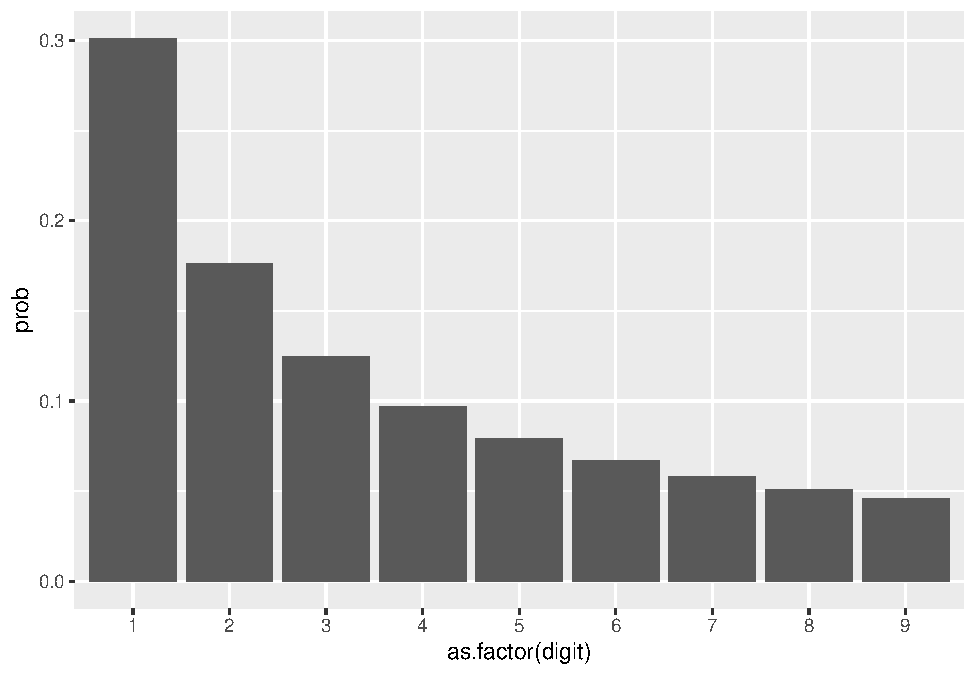
\includegraphics{Audit_Analytics_with-R_files/figure-latex/unnamed-chunk-127-1.pdf}

If we assume the first dataset is an example of a generally real world dataset, then lets look at a completely fictional dataset. For example, lets say in a range of 1 to 999, we randomly sample 1000 numbers and apply the Benford Law, we will notice the following:

\begin{Shaded}
\begin{Highlighting}[]
\NormalTok{benford_sample <-}\StringTok{ }\KeywordTok{data.frame}\NormalTok{(}\DataTypeTok{seq =} \KeywordTok{sample}\NormalTok{(}\DecValTok{1}\OperatorTok{:}\DecValTok{999}\NormalTok{, }\DecValTok{1000}\NormalTok{, }\DataTypeTok{replace =} \OtherTok{TRUE}\NormalTok{))}
\NormalTok{benford_sample}\OperatorTok{$}\NormalTok{leading <-}\StringTok{ }\KeywordTok{as.numeric}\NormalTok{(}\KeywordTok{substr}\NormalTok{(benford_sample}\OperatorTok{$}\NormalTok{seq, }\DecValTok{1}\NormalTok{, }\DecValTok{1}\NormalTok{))}

\NormalTok{benford_sample }\OperatorTok
\StringTok{  }\KeywordTok{group_by}\NormalTok{(leading) }\OperatorTok
\StringTok{  }\KeywordTok{summarize}\NormalTok{(}\DataTypeTok{times_occured =} \KeywordTok{n}\NormalTok{()) }\OperatorTok
\StringTok{  }\KeywordTok{ggplot}\NormalTok{(}\KeywordTok{aes}\NormalTok{(}\DataTypeTok{x =} \KeywordTok{as.factor}\NormalTok{(leading), }\DataTypeTok{y =}\NormalTok{ times_occured)) }\OperatorTok{+}
\StringTok{    }\KeywordTok{geom_col}\NormalTok{()}
\end{Highlighting}
\end{Shaded}

\begin{verbatim}
## `summarise()` ungrouping output (override with `.groups` argument)
\end{verbatim}

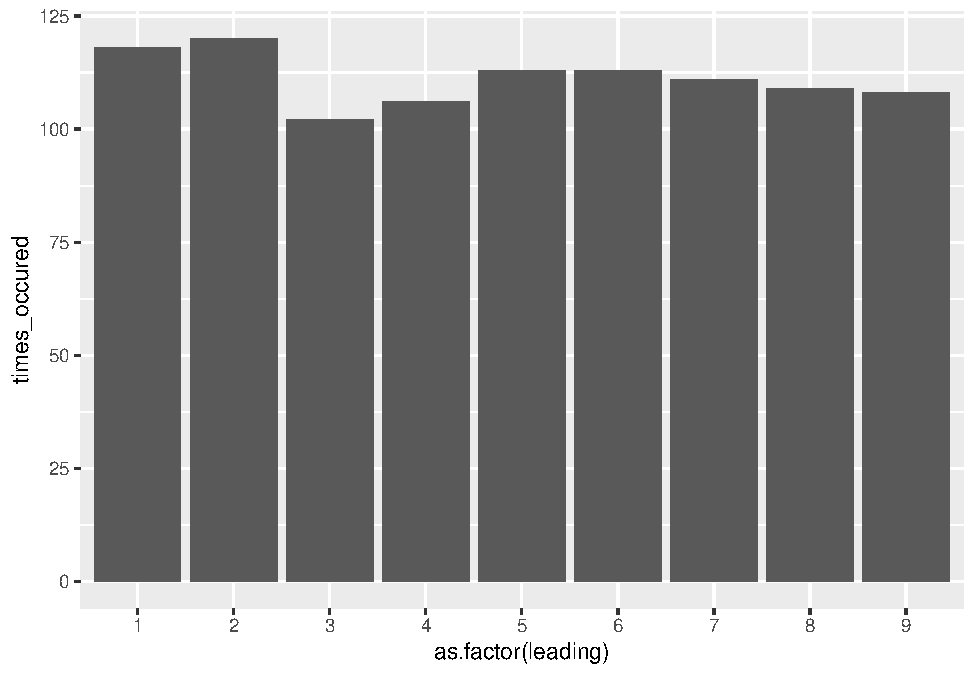
\includegraphics{Audit_Analytics_with-R_files/figure-latex/unnamed-chunk-128-1.pdf}

Notice how uniform the bars appear. The sample we chose was essentially made-up numbers between 1 and 999, the computer would choose these with equal probability, unlike the population of hourly wages, leading to a graph that does not follow the curve of Benford's Law.

\hypertarget{applying-benfords-law}{%
\subsubsection{Applying Benford's Law}\label{applying-benfords-law}}

Several statistical tests exist to determine whether or not a population conforms to Benford's Law. While chi-square tests are numerically `authoritative', remember that the individuals samples will indicate whether or not fraud truly exists.

In application, Benford's Law requires professional judgment, and there can be any number of reasons why a population doesn't follow it. My successful experiences as an auditor have been to chart the actual proportion of leading digits against a curve of the expected outcome, and determine if there are any business reasons that may rationalize a pattern in the data before I perform further sampling.

To calculate the curve, you need to determine the likelihood that each digit should appear. The expected proportion for each digit can be calculated as follows:

\[log_{10}\left( 1 + \frac{1}{d}\right)\]

In R, this is represented as:

\begin{Shaded}
\begin{Highlighting}[]
\NormalTok{d <-}\StringTok{ }\DecValTok{1} \CommentTok{# Leading digit}
\KeywordTok{log10}\NormalTok{(}\DecValTok{1} \OperatorTok{+}\StringTok{ }\DecValTok{1} \OperatorTok{/}\StringTok{ }\NormalTok{d)}
\end{Highlighting}
\end{Shaded}

\begin{verbatim}
## [1] 0.30103
\end{verbatim}

We can create a quick reference curve of the leading digits for Benford's Law:

\begin{Shaded}
\begin{Highlighting}[]
\NormalTok{benford_curve <-}\StringTok{ }\KeywordTok{data.frame}\NormalTok{(}\DataTypeTok{digit =} \DecValTok{1}\OperatorTok{:}\DecValTok{9}\NormalTok{) }\OperatorTok
\StringTok{  }\KeywordTok{mutate}\NormalTok{(}\DataTypeTok{prob =} \KeywordTok{log10}\NormalTok{(}\DecValTok{1} \OperatorTok{+}\StringTok{ }\DecValTok{1} \OperatorTok{/}\StringTok{ }\NormalTok{digit),}
         \DataTypeTok{curve =} \StringTok{'benford'}\NormalTok{)}

\KeywordTok{ggplot}\NormalTok{(benford_curve, }\KeywordTok{aes}\NormalTok{(}\DataTypeTok{x =} \KeywordTok{as.factor}\NormalTok{(digit), }\DataTypeTok{y =}\NormalTok{ prob, }\DataTypeTok{group =}\NormalTok{ curve)) }\OperatorTok{+}
\StringTok{  }\KeywordTok{geom_line}\NormalTok{(}\DataTypeTok{color =} \StringTok{'red'}\NormalTok{) }\OperatorTok{+}
\StringTok{  }\KeywordTok{geom_point}\NormalTok{(}\DataTypeTok{color =} \StringTok{'red'}\NormalTok{)}
\end{Highlighting}
\end{Shaded}

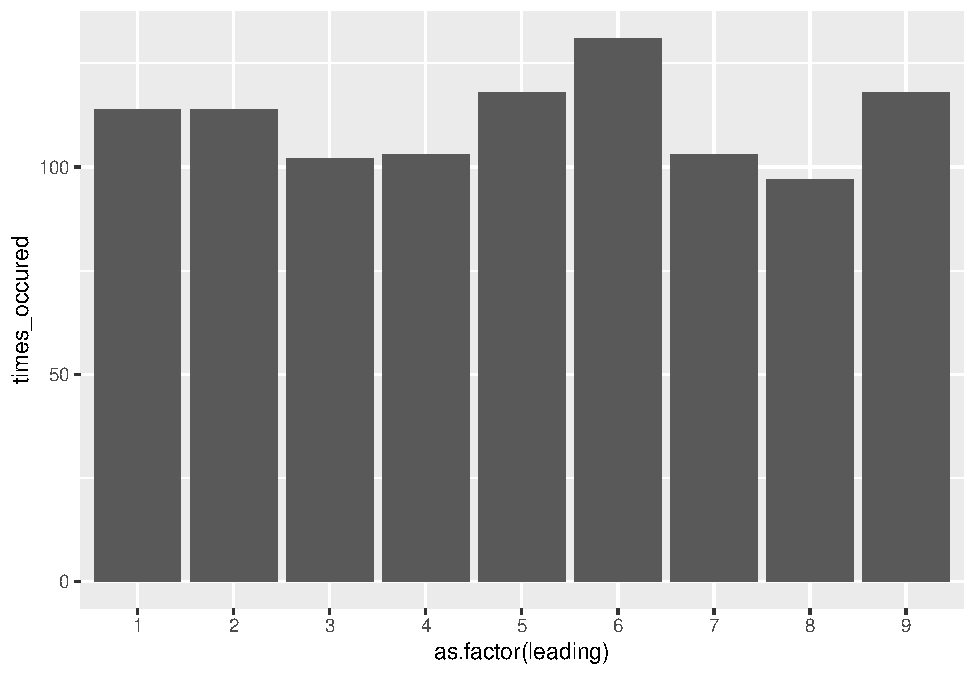
\includegraphics{Audit_Analytics_with-R_files/figure-latex/unnamed-chunk-130-1.pdf}

We can then take any of our populations, create the bar chart, and then apply the expected proportions of Benford's Law to it. Lets take our GL database and create the proportion of how often each leading digit occurs. Note we will try to follow the same variable structure as \texttt{benford\_curve}, as we will combine these on the same chart.

\begin{Shaded}
\begin{Highlighting}[]
\NormalTok{gl }\OperatorTok
\StringTok{  }\KeywordTok{mutate}\NormalTok{(}\DataTypeTok{digit =} \KeywordTok{as.numeric}\NormalTok{(}\KeywordTok{substr}\NormalTok{(amount, }\DecValTok{1}\NormalTok{, }\DecValTok{1}\NormalTok{))) }\OperatorTok
\StringTok{  }\KeywordTok{group_by}\NormalTok{(digit) }\OperatorTok
\StringTok{  }\KeywordTok{summarize}\NormalTok{(}\DataTypeTok{times_occured =} \KeywordTok{n}\NormalTok{()) }\OperatorTok
\StringTok{  }\KeywordTok{mutate}\NormalTok{(}\DataTypeTok{prop =}\NormalTok{ times_occured }\OperatorTok{/}\StringTok{ }\KeywordTok{sum}\NormalTok{(times_occured),}
         \DataTypeTok{curve =} \StringTok{'actual'}\NormalTok{) }\OperatorTok
\StringTok{  }\KeywordTok{ggplot}\NormalTok{(}\KeywordTok{aes}\NormalTok{(}\DataTypeTok{x =} \KeywordTok{as.factor}\NormalTok{(digit), }\DataTypeTok{y =}\NormalTok{ prop)) }\OperatorTok{+}
\StringTok{    }\KeywordTok{geom_col}\NormalTok{()}
\end{Highlighting}
\end{Shaded}

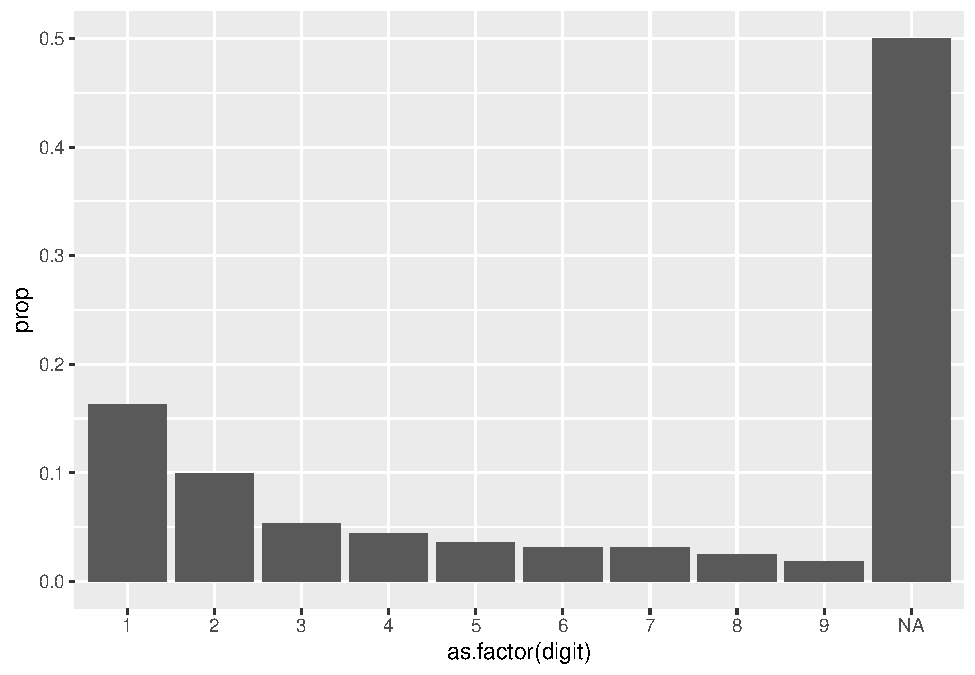
\includegraphics{Audit_Analytics_with-R_files/figure-latex/unnamed-chunk-131-1.pdf}

Notice in our chart that there are several NAs. In our dataset, we have several negative numbers (as journal entry credits as represented with negatives), and extracting the first character using \texttt{substr()} will retrieve the negative symbol. You may choose to perform Benford's Law on the positive and negative numbers, separately or together, transforming the negative numbers with \texttt{abs()}. You can also choose to exclude them, as I do below:

\begin{Shaded}
\begin{Highlighting}[]
\NormalTok{actuals <-}\StringTok{ }\NormalTok{gl }\OperatorTok
\StringTok{  }\KeywordTok{filter}\NormalTok{(amount }\OperatorTok{>}\StringTok{ }\DecValTok{0}\NormalTok{) }\OperatorTok
\StringTok{  }\KeywordTok{mutate}\NormalTok{(}\DataTypeTok{digit =} \KeywordTok{as.numeric}\NormalTok{(}\KeywordTok{substr}\NormalTok{(amount, }\DecValTok{1}\NormalTok{, }\DecValTok{1}\NormalTok{))) }\OperatorTok
\StringTok{  }\KeywordTok{group_by}\NormalTok{(digit) }\OperatorTok
\StringTok{  }\KeywordTok{summarize}\NormalTok{(}\DataTypeTok{times_occured =} \KeywordTok{n}\NormalTok{()) }\OperatorTok
\StringTok{  }\KeywordTok{mutate}\NormalTok{(}\DataTypeTok{prop =}\NormalTok{ times_occured }\OperatorTok{/}\StringTok{ }\KeywordTok{sum}\NormalTok{(times_occured),}
         \DataTypeTok{curve =} \StringTok{'actual'}\NormalTok{) }\OperatorTok
\StringTok{  }\KeywordTok{ggplot}\NormalTok{(}\KeywordTok{aes}\NormalTok{(}\DataTypeTok{x =} \KeywordTok{as.factor}\NormalTok{(digit), }\DataTypeTok{y =}\NormalTok{ prop)) }\OperatorTok{+}
\StringTok{    }\KeywordTok{geom_col}\NormalTok{()}

\NormalTok{actuals}
\end{Highlighting}
\end{Shaded}

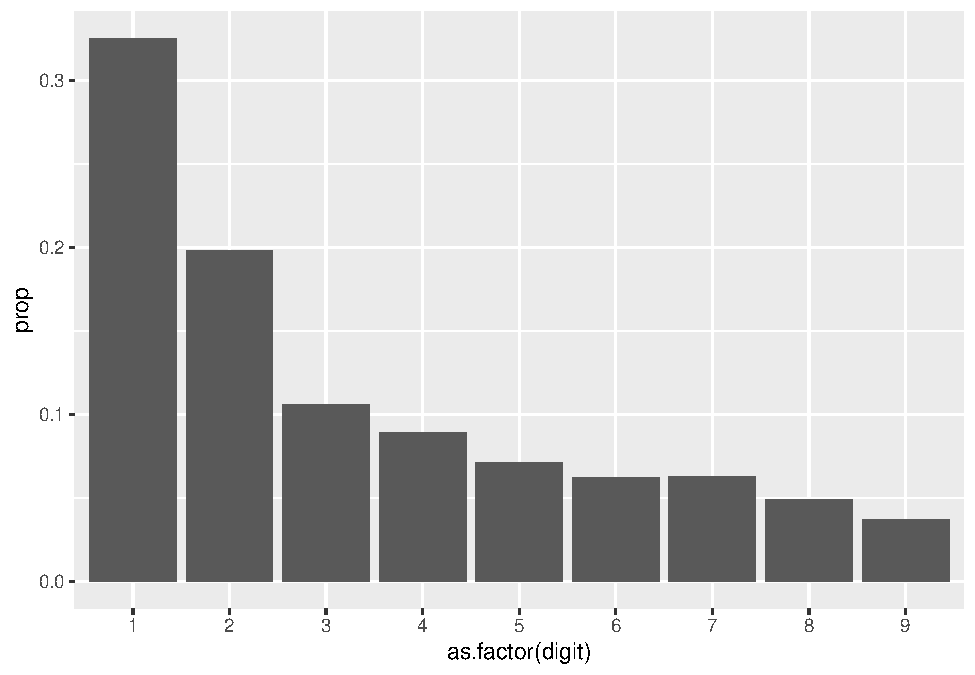
\includegraphics{Audit_Analytics_with-R_files/figure-latex/unnamed-chunk-132-1.pdf}

Now that we have the actual proportions, lets layer on the \texttt{benford\_curve} we created:

\begin{Shaded}
\begin{Highlighting}[]
\NormalTok{actuals }\OperatorTok{+}
\StringTok{  }\KeywordTok{geom_line}\NormalTok{(}\DataTypeTok{data =}\NormalTok{ benford_curve, }\KeywordTok{aes}\NormalTok{(}\DataTypeTok{x =} \KeywordTok{as.factor}\NormalTok{(digit), }\DataTypeTok{y =}\NormalTok{ prob, }\DataTypeTok{group =}\NormalTok{ curve), }\DataTypeTok{color =} \StringTok{'red'}\NormalTok{) }\OperatorTok{+}\StringTok{ }
\StringTok{  }\KeywordTok{geom_point}\NormalTok{(}\DataTypeTok{data =}\NormalTok{ benford_curve, }\KeywordTok{aes}\NormalTok{(}\DataTypeTok{x =} \KeywordTok{as.factor}\NormalTok{(digit), }\DataTypeTok{y =}\NormalTok{ prob), }\DataTypeTok{color =} \StringTok{'red'}\NormalTok{)}
\end{Highlighting}
\end{Shaded}

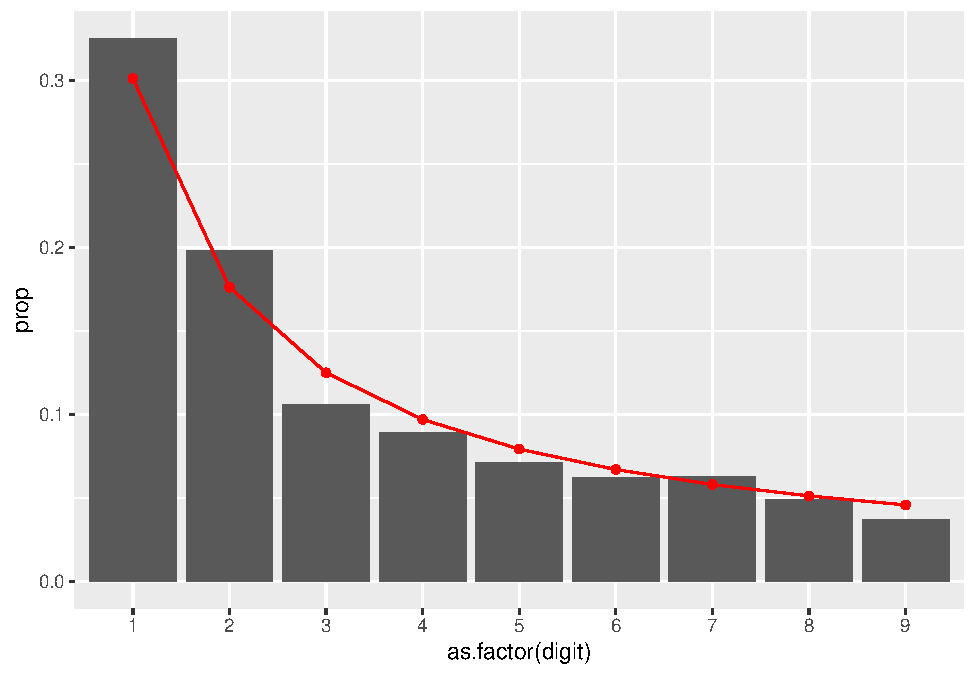
\includegraphics{Audit_Analytics_with-R_files/figure-latex/unnamed-chunk-133-1.pdf}

When you reach this stage, take a moment to pause and understand the business, and if there may be any potential behavours to cause potential curve differences. For example, if there is an approval `limit' that exists at \$1000, you may see a spike of entries at the 9 leading digit.

As with any statistical test, Benford's Law will not give you an answer as to why there may be fraud. There may be both legitimate reasons for why populations do not follow Benford's Law. A higher than expected proportion of leading digits starting with 9 does not mean those numbers starting with 9 are fraudulent.

\hypertarget{more-leading-digits}{%
\subsubsection{More leading digits?}\label{more-leading-digits}}

You can get any number of leading digits to apply Benford's Law - to do so, you need to start on the lowest possible value for the number of digits desired, to remove leading zeros, and extend the sequence to the highest number before a new digit must be added. For example, two leading digits would have a sequence of numbers created from 10:99, and three leading digits would be 100:999:

\begin{Shaded}
\begin{Highlighting}[]
\NormalTok{benford_curve_leading2 <-}\StringTok{ }\KeywordTok{data.frame}\NormalTok{(}\DataTypeTok{digit =} \DecValTok{10}\OperatorTok{:}\DecValTok{99}\NormalTok{) }\OperatorTok
\StringTok{  }\KeywordTok{mutate}\NormalTok{(}\DataTypeTok{prob =} \KeywordTok{log10}\NormalTok{(}\DecValTok{1} \OperatorTok{+}\StringTok{ }\DecValTok{1} \OperatorTok{/}\StringTok{ }\NormalTok{digit),}
         \DataTypeTok{curve =} \StringTok{'benford'}\NormalTok{)}

\KeywordTok{head}\NormalTok{(benford_curve_leading2)}
\end{Highlighting}
\end{Shaded}

\begin{verbatim}
##   digit       prob   curve
## 1    10 0.04139269 benford
## 2    11 0.03778856 benford
## 3    12 0.03476211 benford
## 4    13 0.03218468 benford
## 5    14 0.02996322 benford
##  [ reached 'max' / getOption("max.print") -- omitted 1 rows ]
\end{verbatim}

\begin{Shaded}
\begin{Highlighting}[]
\KeywordTok{tail}\NormalTok{(benford_curve_leading2)}
\end{Highlighting}
\end{Shaded}

\begin{verbatim}
##    digit        prob   curve
## 85    94 0.004595752 benford
## 86    95 0.004547628 benford
## 87    96 0.004500501 benford
## 88    97 0.004454341 benford
## 89    98 0.004409119 benford
##  [ reached 'max' / getOption("max.print") -- omitted 1 rows ]
\end{verbatim}

\hypertarget{relative-size-factor-rsf}{%
\subsection{Relative size factor (RSF)}\label{relative-size-factor-rsf}}

The Relative Size Factor test is the comparison of ``large amounts to a benchmark to see how large they are relative to some norm.'' (\emph{Identifying Anomalies Using the Relative Size Factor Test} \protect\hyperlink{ref-nigrini-forensicanalytics-ch11}{2012}). The calculation is done by taking the largest value divided by the second largest value within a group. Examples of groups include a listing of payables for a vendor, or the expenses completed by an employee. A larger RSF indicates that there was a larger proportional between the largest and second largest invoice.

One test is to determining the vendors top two invoice amounts and their RSF ratio. Recall the \texttt{group\_by()} will perform the calculation at the level requested - adding \texttt{slice\_max()} will select the highest row of values by the group.

\begin{Shaded}
\begin{Highlighting}[]
\NormalTok{top_two_per_vendor <-}\StringTok{ }\NormalTok{gl }\OperatorTok
\StringTok{  }\KeywordTok{filter}\NormalTok{(account }\OperatorTok{==}\StringTok{ 'exp_materials_6000'}\NormalTok{) }\OperatorTok
\StringTok{  }\KeywordTok{select}\NormalTok{(vendor_id, je_num, amount) }\OperatorTok
\StringTok{  }\KeywordTok{group_by}\NormalTok{(vendor_id) }\OperatorTok
\StringTok{  }\KeywordTok{slice_max}\NormalTok{(amount, }\DataTypeTok{n =} \DecValTok{2}\NormalTok{)}

\NormalTok{top_two_per_vendor}
\end{Highlighting}
\end{Shaded}

\begin{verbatim}
## # A tibble: 6 x 3
## # Groups:   vendor_id [3]
##   vendor_id je_num amount
##       <int>  <int>  <dbl>
## 1      2211    140 96355.
## 2      2211    555 57258.
## 3      2612    583 47748.
## 4      2612    337 46066.
## 5      2726    693 88524.
## 6      2726    756 57567.
\end{verbatim}

Since we've identified the top two invoices per \texttt{vendor\_id}, we've artifically also created new max and mins for the group, which we can use to calculate our RSF:

\begin{Shaded}
\begin{Highlighting}[]
\NormalTok{top_two_per_vendor }\OperatorTok
\StringTok{  }\KeywordTok{summarize}\NormalTok{(}\DataTypeTok{rsf =} \KeywordTok{max}\NormalTok{(amount) }\OperatorTok{/}\StringTok{ }\KeywordTok{min}\NormalTok{(amount))}
\end{Highlighting}
\end{Shaded}

\begin{verbatim}
## # A tibble: 3 x 2
##   vendor_id   rsf
##       <int> <dbl>
## 1      2211  1.68
## 2      2612  1.04
## 3      2726  1.54
\end{verbatim}

This test may reveal invoices that may have been miskeyed with extra zeros, or conversely, identify large one-time orders.

\hypertarget{duplicate-invoices}{%
\subsection{Duplicate Invoices}\label{duplicate-invoices}}

Detection of duplicates are a seemingly simple concept. For invoices, find an invoice with the same invoice date and same amount. Experience will tell you that detecting suspected duplicates and generating a list is easy, and unfortunately there will be a significant number of false positives to wade through. We will go through the basics of duplicate detection with invoices, and then determine additional strategies you can apply to rule out unlikely samples. These same strategies can be applied across any type of payable.

The initial approach is built off the Same-Same-Same or Same-Same-Different duplicate detection approach (\emph{Identifying Fraud Using Abnormal Duplications Within Subsets} \protect\hyperlink{ref-nigrini-forensicanalytics-ch12}{2012}). Essentially, you examine for factors where the may be similarities in the key fields, and potentially differences in one of them. Here is a fictional dataset to illustrate how data may be represented.

Note that despite the name, there can be as many `Same' key fields as needed.

\begin{Shaded}
\begin{Highlighting}[]
\NormalTok{invoices <-}\StringTok{ }\KeywordTok{data.frame}\NormalTok{(}\DataTypeTok{system_id =} \DecValTok{1}\OperatorTok{:}\DecValTok{7}\NormalTok{,}
           \DataTypeTok{invoice_id =} \KeywordTok{c}\NormalTok{(}\StringTok{'156'}\NormalTok{, }\StringTok{'156'}\NormalTok{, }\StringTok{'157A'}\NormalTok{, }\StringTok{'157B'}\NormalTok{, }\StringTok{'158'}\NormalTok{, }\StringTok{'159'}\NormalTok{, }\StringTok{'160'}\NormalTok{), }
           \DataTypeTok{date =} \KeywordTok{c}\NormalTok{(}\KeywordTok{as.Date}\NormalTok{(}\StringTok{'2019-01-01'}\NormalTok{), }\KeywordTok{as.Date}\NormalTok{(}\StringTok{'2019-01-01'}\NormalTok{), }\KeywordTok{as.Date}\NormalTok{(}\StringTok{'2019-01-02'}\NormalTok{), }\KeywordTok{as.Date}\NormalTok{(}\StringTok{'2019-01-02'}\NormalTok{), }\KeywordTok{as.Date}\NormalTok{(}\StringTok{'2019-01-03'}\NormalTok{), }\KeywordTok{as.Date}\NormalTok{(}\StringTok{'2019-01-03'}\NormalTok{), }\KeywordTok{as.Date}\NormalTok{(}\StringTok{'2019-01-04'}\NormalTok{)),}
           \DataTypeTok{amount =} \KeywordTok{c}\NormalTok{(}\DecValTok{1000}\NormalTok{, }\DecValTok{1000}\NormalTok{, }\DecValTok{2500}\NormalTok{, }\DecValTok{2500}\NormalTok{, }\DecValTok{3000}\NormalTok{, }\DecValTok{3000}\NormalTok{, }\DecValTok{4000}\NormalTok{),}
           \DataTypeTok{acctcode =} \KeywordTok{c}\NormalTok{(}\DecValTok{6100}\NormalTok{, }\DecValTok{6100}\NormalTok{, }\DecValTok{6200}\NormalTok{, }\DecValTok{6200}\NormalTok{, }\DecValTok{6100}\NormalTok{, }\DecValTok{6200}\NormalTok{, }\DecValTok{6100}\NormalTok{))}

\NormalTok{invoices }\OperatorTok
\StringTok{  }\KeywordTok{gt}\NormalTok{() }\CommentTok{# We'll hide this table-making code in future chunks. For now, its going to make our table prettier}
\end{Highlighting}
\end{Shaded}

\captionsetup[table]{labelformat=empty,skip=1pt}
\begin{longtable}{cllrr}
\toprule
system\_id & invoice\_id & date & amount & acctcode \\ 
\midrule
1 & 156 & 2019-01-01 & 1000 & 6100 \\ 
2 & 156 & 2019-01-01 & 1000 & 6100 \\ 
3 & 157A & 2019-01-02 & 2500 & 6200 \\ 
4 & 157B & 2019-01-02 & 2500 & 6200 \\ 
5 & 158 & 2019-01-03 & 3000 & 6100 \\ 
6 & 159 & 2019-01-03 & 3000 & 6200 \\ 
7 & 160 & 2019-01-04 & 4000 & 6100 \\ 
\bottomrule
\end{longtable}

\hypertarget{same-same-same}{%
\subsubsection{Same-Same-Same}\label{same-same-same}}

To run our Same-Same-Same test, we would collect the key fields we would like to use. In this case, the invoice, date and amount could qualify as key fields - Same Invoice ID, Same Date, Same Amount. You would summarize by how often that combination appears, only keeping items that match more than once:

\begin{Shaded}
\begin{Highlighting}[]
\NormalTok{dupes_set1 <-}\StringTok{ }\NormalTok{invoices }\OperatorTok
\StringTok{  }\KeywordTok{group_by}\NormalTok{(invoice_id, date, amount) }\OperatorTok
\StringTok{  }\KeywordTok{summarize}\NormalTok{(}\DataTypeTok{times_occured =} \KeywordTok{n}\NormalTok{()) }\OperatorTok
\StringTok{  }\KeywordTok{filter}\NormalTok{(times_occured }\OperatorTok{>}\StringTok{ }\DecValTok{1}\NormalTok{) }\OperatorTok
\StringTok{  }\KeywordTok{ungroup}\NormalTok{()}
\end{Highlighting}
\end{Shaded}

\captionsetup[table]{labelformat=empty,skip=1pt}
\begin{longtable}{llrc}
\toprule
invoice\_id & date & amount & times\_occured \\ 
\midrule
156 & 2019-01-01 & 1000 & 2 \\ 
\bottomrule
\end{longtable}

To keep track of which invoices meet specific criteria, we will then join this information to the main dataset. This way, you'll maintain a library of invoices that meet multiple criteria. First off, lets keep keep all the duplicate keys we summarized on, plus a unique identifier so we can match the pairs:

\begin{Shaded}
\begin{Highlighting}[]
\NormalTok{dupes_set1 <-}\StringTok{ }\NormalTok{dupes_set1 }\OperatorTok\StringTok{ }
\StringTok{  }\KeywordTok{ungroup}\NormalTok{() }\OperatorTok\StringTok{ }\CommentTok{# Remove the grouping aspect, which affects the ranking by row_number()}
\StringTok{  }\KeywordTok{mutate}\NormalTok{(}\DataTypeTok{t_dupes1 =} \KeywordTok{row_number}\NormalTok{()) }
\end{Highlighting}
\end{Shaded}

\captionsetup[table]{labelformat=empty,skip=1pt}
\begin{longtable}{llrcc}
\toprule
invoice\_id & date & amount & times\_occured & t\_dupes1 \\ 
\midrule
156 & 2019-01-01 & 1000 & 2 & 1 \\ 
\bottomrule
\end{longtable}

Then bring it into our invoices dataset:

\begin{Shaded}
\begin{Highlighting}[]
\NormalTok{dupes_set1 <-}\StringTok{ }\NormalTok{dupes_set1 }\OperatorTok
\StringTok{  }\KeywordTok{select}\NormalTok{(}\OperatorTok{-}\NormalTok{times_occured) }\CommentTok{# Unneeded for final result}

\NormalTok{invoices <-}\StringTok{ }\NormalTok{invoices }\OperatorTok
\StringTok{  }\KeywordTok{left_join}\NormalTok{(dupes_set1, }\DataTypeTok{by =} \KeywordTok{c}\NormalTok{(}\StringTok{'invoice_id'}\NormalTok{, }\StringTok{'date'}\NormalTok{, }\StringTok{'amount'}\NormalTok{))}
\end{Highlighting}
\end{Shaded}

\captionsetup[table]{labelformat=empty,skip=1pt}
\begin{longtable}{cllrrc}
\toprule
system\_id & invoice\_id & date & amount & acctcode & t\_dupes1 \\ 
\midrule
1 & 156 & 2019-01-01 & 1000 & 6100 & 1 \\ 
2 & 156 & 2019-01-01 & 1000 & 6100 & 1 \\ 
3 & 157A & 2019-01-02 & 2500 & 6200 & NA \\ 
4 & 157B & 2019-01-02 & 2500 & 6200 & NA \\ 
5 & 158 & 2019-01-03 & 3000 & 6100 & NA \\ 
6 & 159 & 2019-01-03 & 3000 & 6200 & NA \\ 
7 & 160 & 2019-01-04 & 4000 & 6100 & NA \\ 
\bottomrule
\end{longtable}

\hypertarget{same-same-different}{%
\subsubsection{Same-Same-Different}\label{same-same-different}}

For the Same-Same-Different test, we have to add an extra step. We still collect the key fields we would like to use. In this case, perhaps we would like to check for duplicates on the same date and same amount, but now we're looking for different invoice\_ids. Therefore, Same Date, Same Amount, Different Invoice\_id.

First, lets detect the duplicates on our key fields:

\begin{Shaded}
\begin{Highlighting}[]
\NormalTok{dupes_set2 <-}\StringTok{ }\NormalTok{invoices }\OperatorTok
\StringTok{  }\KeywordTok{group_by}\NormalTok{(invoice_id, date, amount) }\OperatorTok
\StringTok{  }\KeywordTok{summarize}\NormalTok{(}\DataTypeTok{times_occured =} \KeywordTok{n}\NormalTok{()) }\OperatorTok
\StringTok{  }\KeywordTok{ungroup}\NormalTok{()}
\end{Highlighting}
\end{Shaded}

\captionsetup[table]{labelformat=empty,skip=1pt}
\begin{longtable}{llrc}
\toprule
invoice\_id & date & amount & times\_occured \\ 
\midrule
156 & 2019-01-01 & 1000 & 2 \\ 
157A & 2019-01-02 & 2500 & 1 \\ 
157B & 2019-01-02 & 2500 & 1 \\ 
158 & 2019-01-03 & 3000 & 1 \\ 
159 & 2019-01-03 & 3000 & 1 \\ 
160 & 2019-01-04 & 4000 & 1 \\ 
\bottomrule
\end{longtable}

Then, you perform another \texttt{group\_by}, but this time just on the ones that are the same. In this case, that would be Date and Amount.

\begin{Shaded}
\begin{Highlighting}[]
\NormalTok{dupes_set2 <-}\StringTok{ }\NormalTok{dupes_set2 }\OperatorTok\StringTok{ }\CommentTok{# Remove the grouping aspect, which is kept by default in dplyr}
\StringTok{  }\KeywordTok{group_by}\NormalTok{(date, amount) }\OperatorTok\StringTok{ }\CommentTok{# Second set of reductions, but this time, find how many unique invoice ids there are per date-amount}
\StringTok{  }\KeywordTok{summarize}\NormalTok{(}\DataTypeTok{times_occured =} \KeywordTok{n}\NormalTok{()) }\OperatorTok
\StringTok{  }\KeywordTok{filter}\NormalTok{(times_occured }\OperatorTok{>}\StringTok{ }\DecValTok{1}\NormalTok{) }\OperatorTok
\StringTok{  }\KeywordTok{ungroup}\NormalTok{()}
\end{Highlighting}
\end{Shaded}

\captionsetup[table]{labelformat=empty,skip=1pt}
\begin{longtable}{lrc}
\toprule
date & amount & times\_occured \\ 
\midrule
2019-01-02 & 2500 & 2 \\ 
2019-01-03 & 3000 & 2 \\ 
\bottomrule
\end{longtable}

This approach is unique but intuitive. By taking all possible `same' combinations, we've effectively grouped any sort of duplicate \texttt{invoice\_id} we may have already had. We then ungroup and resummarize without the \texttt{invoice\_id}, which tells us how many times the \texttt{invoice\_id} is different within the new group.

Lets save this information into our invoice table again:

\begin{Shaded}
\begin{Highlighting}[]
\NormalTok{dupes_set2 <-}\StringTok{ }\NormalTok{dupes_set2 }\OperatorTok
\StringTok{  }\KeywordTok{mutate}\NormalTok{(}\DataTypeTok{t_dupes2 =} \KeywordTok{row_number}\NormalTok{()) }\OperatorTok
\StringTok{  }\KeywordTok{select}\NormalTok{(}\OperatorTok{-}\NormalTok{times_occured)}

\NormalTok{invoices <-}\StringTok{ }\NormalTok{invoices }\OperatorTok
\StringTok{  }\KeywordTok{left_join}\NormalTok{(dupes_set2, }\DataTypeTok{by =} \KeywordTok{c}\NormalTok{(}\StringTok{'date'}\NormalTok{, }\StringTok{'amount'}\NormalTok{))}
\end{Highlighting}
\end{Shaded}

\captionsetup[table]{labelformat=empty,skip=1pt}
\begin{longtable}{cllrrcc}
\toprule
system\_id & invoice\_id & date & amount & acctcode & t\_dupes1 & t\_dupes2 \\ 
\midrule
1 & 156 & 2019-01-01 & 1000 & 6100 & 1 & NA \\ 
2 & 156 & 2019-01-01 & 1000 & 6100 & 1 & NA \\ 
3 & 157A & 2019-01-02 & 2500 & 6200 & NA & 1 \\ 
4 & 157B & 2019-01-02 & 2500 & 6200 & NA & 1 \\ 
5 & 158 & 2019-01-03 & 3000 & 6100 & NA & 2 \\ 
6 & 159 & 2019-01-03 & 3000 & 6200 & NA & 2 \\ 
7 & 160 & 2019-01-04 & 4000 & 6100 & NA & NA \\ 
\bottomrule
\end{longtable}

The beauty of this method is that, after you've run all the scenarios you prefer, you can rapidly assess each invoice and see what duplicate criteria they match. Ideally, you would balance having tests that are very general (same date, same amount) with tests of high precision (same date, same amount, and different account codes).

\hypertarget{aggregating-results}{%
\subsubsection{Aggregating results}\label{aggregating-results}}

To derive the final list, becai effective to filter the results based on the \texttt{dupes} columns.

Starting with the invoices we've identified, we'll first group by unique \texttt{system\_id} we've created, allowing us to perform calculations on unique rows. To determine if any test did return something, we will take a \texttt{sum} of any number of columns that return a TRUE (with a value of 1 when coerced from logical to numeric). Then, we want to calculate this on multiple columns, specifically with the name starting with \texttt{dupes}, so we will use \texttt{across()} with \texttt{starts\_with()}.

\begin{Shaded}
\begin{Highlighting}[]
\NormalTok{invoices }\OperatorTok
\StringTok{  }\KeywordTok{rowwise}\NormalTok{(system_id) }\OperatorTok
\StringTok{  }\KeywordTok{mutate}\NormalTok{(}\DataTypeTok{dupes =} \KeywordTok{sum}\NormalTok{(}\KeywordTok{across}\NormalTok{(}\KeywordTok{starts_with}\NormalTok{(}\StringTok{'t_dupes'}\NormalTok{)) }\OperatorTok{>=}\StringTok{ }\DecValTok{1}\NormalTok{, }\DataTypeTok{na.rm =} \OtherTok{TRUE}\NormalTok{)) }\OperatorTok
\StringTok{  }\KeywordTok{ungroup}\NormalTok{() }\OperatorTok
\StringTok{  }\KeywordTok{filter}\NormalTok{(dupes }\OperatorTok{>}\StringTok{ }\DecValTok{0}\NormalTok{) }\OperatorTok
\StringTok{  }\KeywordTok{gt}\NormalTok{()}
\end{Highlighting}
\end{Shaded}

\captionsetup[table]{labelformat=empty,skip=1pt}
\begin{longtable}{cllrrccc}
\toprule
system\_id & invoice\_id & date & amount & acctcode & t\_dupes1 & t\_dupes2 & dupes \\ 
\midrule
1 & 156 & 2019-01-01 & 1000 & 6100 & 1 & NA & 1 \\ 
2 & 156 & 2019-01-01 & 1000 & 6100 & 1 & NA & 1 \\ 
3 & 157A & 2019-01-02 & 2500 & 6200 & NA & 1 & 1 \\ 
4 & 157B & 2019-01-02 & 2500 & 6200 & NA & 1 & 1 \\ 
5 & 158 & 2019-01-03 & 3000 & 6100 & NA & 2 & 1 \\ 
6 & 159 & 2019-01-03 & 3000 & 6200 & NA & 2 & 1 \\ 
\bottomrule
\end{longtable}

This approach is powerful, yet flexible. By maintaining our approach of having a main \texttt{invoice} dataset with all the matches, any new tests we add starting with the column name \texttt{dupes} will be included. For example, if we inserted a higher precision test of same invoice date, amount, and account code, we'll see our counts go up:

\begin{Shaded}
\begin{Highlighting}[]
\NormalTok{dupes_set3 <-}\StringTok{ }\NormalTok{invoices }\OperatorTok
\StringTok{  }\KeywordTok{group_by}\NormalTok{(date, amount, acctcode) }\OperatorTok
\StringTok{  }\KeywordTok{summarize}\NormalTok{(}\DataTypeTok{times_occured =} \KeywordTok{n}\NormalTok{()) }\OperatorTok
\StringTok{  }\KeywordTok{filter}\NormalTok{(times_occured }\OperatorTok{>}\StringTok{ }\DecValTok{1}\NormalTok{) }\OperatorTok
\StringTok{  }\KeywordTok{ungroup}\NormalTok{() }\OperatorTok\StringTok{ }\CommentTok{# Remove the grouping aspect, which affects the ranking by row_number()}
\StringTok{  }\KeywordTok{mutate}\NormalTok{(}\DataTypeTok{t_dupes3 =} \KeywordTok{row_number}\NormalTok{()) }\OperatorTok
\StringTok{  }\KeywordTok{select}\NormalTok{(}\OperatorTok{-}\NormalTok{times_occured)}

\NormalTok{invoices <-}\StringTok{ }\NormalTok{invoices }\OperatorTok
\StringTok{  }\KeywordTok{left_join}\NormalTok{(dupes_set3, }\DataTypeTok{by =} \KeywordTok{c}\NormalTok{(}\StringTok{'date'}\NormalTok{, }\StringTok{'amount'}\NormalTok{, }\StringTok{'acctcode'}\NormalTok{)) }

\NormalTok{invoices }\OperatorTok
\StringTok{  }\KeywordTok{rowwise}\NormalTok{(system_id) }\OperatorTok
\StringTok{  }\KeywordTok{mutate}\NormalTok{(}\DataTypeTok{t_dupesmatched =} \KeywordTok{sum}\NormalTok{(}\KeywordTok{across}\NormalTok{(}\KeywordTok{starts_with}\NormalTok{(}\StringTok{'t_dupes'}\NormalTok{)) }\OperatorTok{>=}\StringTok{ }\DecValTok{1}\NormalTok{, }\DataTypeTok{na.rm =} \OtherTok{TRUE}\NormalTok{)) }\OperatorTok
\StringTok{  }\KeywordTok{ungroup}\NormalTok{() }\OperatorTok
\StringTok{  }\KeywordTok{filter}\NormalTok{(t_dupesmatched }\OperatorTok{>}\StringTok{ }\DecValTok{0}\NormalTok{) }\OperatorTok
\StringTok{  }\KeywordTok{gt}\NormalTok{()}
\end{Highlighting}
\end{Shaded}

\captionsetup[table]{labelformat=empty,skip=1pt}
\begin{longtable}{cllrrcccc}
\toprule
system\_id & invoice\_id & date & amount & acctcode & t\_dupes1 & t\_dupes2 & t\_dupes3 & t\_dupesmatched \\ 
\midrule
1 & 156 & 2019-01-01 & 1000 & 6100 & 1 & NA & 1 & 2 \\ 
2 & 156 & 2019-01-01 & 1000 & 6100 & 1 & NA & 1 & 2 \\ 
3 & 157A & 2019-01-02 & 2500 & 6200 & NA & 1 & 2 & 2 \\ 
4 & 157B & 2019-01-02 & 2500 & 6200 & NA & 1 & 2 & 2 \\ 
5 & 158 & 2019-01-03 & 3000 & 6100 & NA & 2 & NA & 1 \\ 
6 & 159 & 2019-01-03 & 3000 & 6200 & NA & 2 & NA & 1 \\ 
\bottomrule
\end{longtable}

\hypertarget{ruling-out-false-positives}{%
\subsubsection{Ruling out false positives}\label{ruling-out-false-positives}}

Up to now, you've identified duplicates via the Same-Same-Same and Same-Same-Different methods. Perhaps in your own work, you've gone ahead and tested potential duplicates, and then realized there is some business logic you didn't capture that may have nullified the potential duplicate, saving you time and effort.

A common reason for a false positive is that the company may have already received a refund for the invoice. In this case, its more practical to identify and remove invoices that have had refunds in the original invoice population prior to processing, using an \texttt{anti\_join()}. For example, if invoice 156 with a system\_id of \texttt{2} was already removed, you could refine the invoice population before executing additional tests.

\begin{Shaded}
\begin{Highlighting}[]
\NormalTok{refunds <-}\StringTok{ }\KeywordTok{data.frame}\NormalTok{(}\DataTypeTok{system_id =} \DecValTok{2}\NormalTok{) }\CommentTok{# A table of credits or refunds}

\NormalTok{new_invoices <-}\StringTok{ }\NormalTok{invoices }\OperatorTok
\StringTok{  }\KeywordTok{anti_join}\NormalTok{(refunds, }\DataTypeTok{by =} \StringTok{'system_id'}\NormalTok{) }\OperatorTok\StringTok{ }\CommentTok{# Remove refunds}
\StringTok{  }\KeywordTok{select}\NormalTok{(system_id, invoice_id, date, amount, acctcode)}

\NormalTok{new_invoices }\OperatorTok\StringTok{ }
\StringTok{  }\KeywordTok{gt}\NormalTok{()}
\end{Highlighting}
\end{Shaded}

\captionsetup[table]{labelformat=empty,skip=1pt}
\begin{longtable}{cllrr}
\toprule
system\_id & invoice\_id & date & amount & acctcode \\ 
\midrule
1 & 156 & 2019-01-01 & 1000 & 6100 \\ 
3 & 157A & 2019-01-02 & 2500 & 6200 \\ 
4 & 157B & 2019-01-02 & 2500 & 6200 \\ 
5 & 158 & 2019-01-03 & 3000 & 6100 \\ 
6 & 159 & 2019-01-03 & 3000 & 6200 \\ 
7 & 160 & 2019-01-04 & 4000 & 6100 \\ 
\bottomrule
\end{longtable}

A duplicate may also be ruled out because because of a minor field that wasn't used. If you examine lines 5 and 6, you'll see that that this invoice was picked up because of the same \texttt{date} \& \texttt{amount}, with a different \texttt{invoice\_id}. You may have noticed that the \texttt{acctcode} is different, representing that the invoice was being allocated to a different cost center. After inquiring with the business, you may determine this behavior is normal. Its easier add another test to accommodate for this scenario, following the Same-Same-Different approach, to help increase the accuracy of test:

\begin{Shaded}
\begin{Highlighting}[]
\NormalTok{dupes_set4 <-}\StringTok{ }\NormalTok{invoices }\OperatorTok
\StringTok{  }\KeywordTok{group_by}\NormalTok{(invoice_id, date, amount, acctcode) }\OperatorTok
\StringTok{  }\KeywordTok{summarize}\NormalTok{(}\DataTypeTok{times_occured =} \KeywordTok{n}\NormalTok{()) }\OperatorTok
\StringTok{  }\KeywordTok{ungroup}\NormalTok{() }\OperatorTok\StringTok{ }\CommentTok{# Remove the grouping aspect, which is kept by default in dplyr}
\StringTok{  }\KeywordTok{group_by}\NormalTok{(date, amount, acctcode) }\OperatorTok\StringTok{ }\CommentTok{# Second set of reductions, but this time, find how many unique invoice ids there are per date-amount}
\StringTok{  }\KeywordTok{summarize}\NormalTok{(}\DataTypeTok{times_occured =} \KeywordTok{n}\NormalTok{()) }\OperatorTok
\StringTok{  }\KeywordTok{filter}\NormalTok{(times_occured }\OperatorTok{>}\StringTok{ }\DecValTok{1}\NormalTok{) }\OperatorTok
\StringTok{  }\KeywordTok{ungroup}\NormalTok{() }\OperatorTok\StringTok{ }\CommentTok{# Remove the grouping aspect, which affects the ranking by row_number()}
\StringTok{  }\KeywordTok{mutate}\NormalTok{(}\DataTypeTok{t_dupes4 =} \KeywordTok{row_number}\NormalTok{()) }\OperatorTok
\StringTok{  }\KeywordTok{select}\NormalTok{(}\OperatorTok{-}\NormalTok{times_occured)}

\NormalTok{invoices <-}\StringTok{ }\NormalTok{invoices }\OperatorTok
\StringTok{  }\KeywordTok{left_join}\NormalTok{(dupes_set4, }\DataTypeTok{by =} \KeywordTok{c}\NormalTok{(}\StringTok{'date'}\NormalTok{, }\StringTok{'amount'}\NormalTok{, }\StringTok{'acctcode'}\NormalTok{))}

\NormalTok{invoices }\OperatorTok
\StringTok{  }\KeywordTok{gt}\NormalTok{()}
\end{Highlighting}
\end{Shaded}

\captionsetup[table]{labelformat=empty,skip=1pt}
\begin{longtable}{cllrrcccc}
\toprule
system\_id & invoice\_id & date & amount & acctcode & t\_dupes1 & t\_dupes2 & t\_dupes3 & t\_dupes4 \\ 
\midrule
1 & 156 & 2019-01-01 & 1000 & 6100 & 1 & NA & 1 & NA \\ 
2 & 156 & 2019-01-01 & 1000 & 6100 & 1 & NA & 1 & NA \\ 
3 & 157A & 2019-01-02 & 2500 & 6200 & NA & 1 & 2 & 1 \\ 
4 & 157B & 2019-01-02 & 2500 & 6200 & NA & 1 & 2 & 1 \\ 
5 & 158 & 2019-01-03 & 3000 & 6100 & NA & 2 & NA & NA \\ 
6 & 159 & 2019-01-03 & 3000 & 6200 & NA & 2 & NA & NA \\ 
7 & 160 & 2019-01-04 & 4000 & 6100 & NA & NA & NA & NA \\ 
\bottomrule
\end{longtable}

\hypertarget{detecting-gaps-in-sequences}{%
\subsection{Detecting gaps in sequences}\label{detecting-gaps-in-sequences}}

A sequential test is commonly used for cheques, specifically to determine which ones are missing from a cheque run. They are also useful for measuring a level of dependency that a vendor relies upon a company, assuming the vendor issue invoices sequentially as well.

As an example, lets say we create a register with 1000 cheques. You can start with any minimum and maximum range:

\begin{Shaded}
\begin{Highlighting}[]
\NormalTok{register <-}\StringTok{ }\KeywordTok{seq}\NormalTok{(}\DecValTok{1020}\NormalTok{, }\DecValTok{2019}\NormalTok{)}
\KeywordTok{length}\NormalTok{(register)}
\end{Highlighting}
\end{Shaded}

\begin{verbatim}
## [1] 1000
\end{verbatim}

\begin{Shaded}
\begin{Highlighting}[]
\KeywordTok{range}\NormalTok{(register)}
\end{Highlighting}
\end{Shaded}

\begin{verbatim}
## [1] 1020 2019
\end{verbatim}

And if we were to create a listing of all cheques we have written, we could simulate perhaps 50 cheques that were taken out:

\begin{Shaded}
\begin{Highlighting}[]
\KeywordTok{set.seed}\NormalTok{(}\DecValTok{123}\NormalTok{)}
\NormalTok{cheques_issued <-}\StringTok{ }\KeywordTok{sample}\NormalTok{(register, }\DataTypeTok{size =} \DecValTok{975}\NormalTok{)}
\end{Highlighting}
\end{Shaded}

To detect which cheques have been taken out, we can check the difference between our sets using \texttt{setdiff()} - that is, if we compare our original cheque register to the cheques issued, we can see which ones were missing:

\begin{Shaded}
\begin{Highlighting}[]
\NormalTok{missing <-}\StringTok{ }\KeywordTok{setdiff}\NormalTok{(register, cheques_issued)}

\NormalTok{missing}
\end{Highlighting}
\end{Shaded}

\begin{verbatim}
##  [1] 1026 1062 1079 1166 1201 1302 1375 1378 1385 1387 1455 1493 1503 1504 1510
##  [ reached getOption("max.print") -- omitted 10 entries ]
\end{verbatim}

If you wanted to know which ones were sequential, you could check the differences between each missing cheque. In this case, it would be a \texttt{lag()} calculation first, to find the difference between each row:

\begin{Shaded}
\begin{Highlighting}[]
\KeywordTok{data.frame}\NormalTok{(missing) }\OperatorTok
\StringTok{  }\KeywordTok{mutate}\NormalTok{(}\DataTypeTok{gap_between =}\NormalTok{ missing }\OperatorTok{-}\StringTok{ }\KeywordTok{lag}\NormalTok{(missing))}
\end{Highlighting}
\end{Shaded}

\begin{verbatim}
##   missing gap_between
## 1    1026          NA
## 2    1062          36
## 3    1079          17
## 4    1166          87
## 5    1201          35
## 6    1302         101
## 7    1375          73
##  [ reached 'max' / getOption("max.print") -- omitted 18 rows ]
\end{verbatim}

And finally, since we want to know which sequential cheques were missing, we could filter and look for any rows that had only a difference of one, implying one missing cheque. Since we want chains, we also want to look ahead with \texttt{lead()} since

\begin{Shaded}
\begin{Highlighting}[]
\KeywordTok{data.frame}\NormalTok{(missing) }\OperatorTok
\StringTok{  }\KeywordTok{mutate}\NormalTok{(}\DataTypeTok{gap_between =}\NormalTok{ missing }\OperatorTok{-}\StringTok{ }\KeywordTok{lag}\NormalTok{(missing)) }\OperatorTok
\StringTok{  }\KeywordTok{filter}\NormalTok{(}\KeywordTok{lead}\NormalTok{(gap_between) }\OperatorTok{==}\StringTok{ }\DecValTok{1} \OperatorTok{|}\StringTok{ }\CommentTok{# Chooses the first row in the chain, by looking at the next row to see if its equal to one}
\StringTok{         }\NormalTok{gap_between }\OperatorTok{==}\DecValTok{1}\NormalTok{ ) }\CommentTok{# Any subsequent numbers will always have a difference of 1}
\end{Highlighting}
\end{Shaded}

\begin{verbatim}
##   missing gap_between
## 1    1503          10
## 2    1504           1
## 3    1661          86
## 4    1662           1
\end{verbatim}

\hypertarget{test-searchtext}{%
\section{Search text}\label{test-searchtext}}

For typical fields in a structured dataset, it is straight forward to \texttt{filter()} on a field to isolate specific traits, like usernames or accounts. However, a great deal of information kept within a database is also unstructured, where the user is allowed to input their own information as they see fit, like description or comment fields. While this information is messy, free-form and generally user-generated, it usually contains a valuable trove of information

To scan these unstructured datasets, you need an effective, powerful and rapid method for analysis. Key word searches are an effective method of isolating high-value entries, especially when examining invoices, journal entries, or other datasets where the data may be inconsistent. We may also be interested in words that imply an action like override, or simply looking for mentions of a name in a comment field.

\hypertarget{regex-basics}{%
\subsection{Regex basics}\label{regex-basics}}

We will need to expand our skill set and dabble in regular expression, also known as \textbf{regex}. Regular expression is another language that specializes in the searching of patterns, specifically within text fields.

To use regex effectively, you need to consider the pattern of the text to look for, and the field you want to search up. Lets start off by listing of Canadian capitial cities and their provinces:

\begin{Shaded}
\begin{Highlighting}[]
\NormalTok{canada <-}\StringTok{ }\KeywordTok{data.frame}\NormalTok{(}\DataTypeTok{province =} \KeywordTok{c}\NormalTok{(}\StringTok{"Newfoundland and Labrador"}\NormalTok{, }\StringTok{"Prince Edward Island"}\NormalTok{, }\StringTok{"Nova Scotia"}\NormalTok{, }\StringTok{"New Brunswick"}\NormalTok{, }\StringTok{"Quebec"}\NormalTok{, }\StringTok{"Ontario"}\NormalTok{, }\StringTok{"Manitoba"}\NormalTok{, }\StringTok{"Saskatchewan"}\NormalTok{, }\StringTok{"Alberta"}\NormalTok{, }\StringTok{"British Columbia"}\NormalTok{, }\StringTok{"Nunavut"}\NormalTok{, }\StringTok{"Northwest Territories"}\NormalTok{, }\StringTok{"Yukon Territory"}\NormalTok{),}
                     \DataTypeTok{capital =} \KeywordTok{c}\NormalTok{(}\StringTok{"St. John's"}\NormalTok{, }\StringTok{"Charlottetown"}\NormalTok{, }\StringTok{"Halifax"}\NormalTok{, }\StringTok{"Fredericton"}\NormalTok{, }\StringTok{"Québec City"}\NormalTok{, }\StringTok{"Toronto"}\NormalTok{, }\StringTok{"Winnipeg"}\NormalTok{, }\StringTok{"Regina"}\NormalTok{, }\StringTok{"Edmonton"}\NormalTok{, }\StringTok{"Victoria"}\NormalTok{, }\StringTok{"Iqaluit"}\NormalTok{, }\StringTok{"Yellowknife"}\NormalTok{, }\StringTok{"Whitehorse"}\NormalTok{))}

\KeywordTok{print}\NormalTok{(canada)}
\end{Highlighting}
\end{Shaded}

\begin{verbatim}
##                    province       capital
## 1 Newfoundland and Labrador    St. John's
## 2      Prince Edward Island Charlottetown
## 3               Nova Scotia       Halifax
## 4             New Brunswick   Fredericton
## 5                    Quebec   Québec City
## 6                   Ontario       Toronto
## 7                  Manitoba      Winnipeg
##  [ reached 'max' / getOption("max.print") -- omitted 6 rows ]
\end{verbatim}

Lets say we wanted to find the city of Edmonton in the column of capitals. We'll use R base function \texttt{grepl()}, which needs a string to search up and a pattern to look into. It returns a logical vector, telling us where matches occur.

\begin{Shaded}
\begin{Highlighting}[]
\KeywordTok{grepl}\NormalTok{(}\StringTok{'Edmonton'}\NormalTok{, canada}\OperatorTok{$}\NormalTok{capital)}
\end{Highlighting}
\end{Shaded}

\begin{verbatim}
##  [1] FALSE FALSE FALSE FALSE FALSE FALSE FALSE FALSE  TRUE FALSE FALSE FALSE
## [13] FALSE
\end{verbatim}

There is only one row that matches our test. We can use this to further isolate our data:

\begin{Shaded}
\begin{Highlighting}[]
\NormalTok{canada }\OperatorTok
\StringTok{  }\KeywordTok{filter}\NormalTok{(}\KeywordTok{grepl}\NormalTok{(}\StringTok{'Edmonton'}\NormalTok{, capital))}
\end{Highlighting}
\end{Shaded}

\begin{verbatim}
##   province  capital
## 1  Alberta Edmonton
\end{verbatim}

What if you wanted to find two words? Separate words with the \texttt{\textbar{}} (pipe) character, which stands for `or', and you chain as many words as you like:

\begin{Shaded}
\begin{Highlighting}[]
\NormalTok{canada }\OperatorTok
\StringTok{  }\KeywordTok{filter}\NormalTok{(}\KeywordTok{grepl}\NormalTok{(}\StringTok{'Charlottetown|Regina'}\NormalTok{, capital))}
\end{Highlighting}
\end{Shaded}

\begin{verbatim}
##               province       capital
## 1 Prince Edward Island Charlottetown
## 2         Saskatchewan        Regina
\end{verbatim}

Regular expressions are powerful because you can customize them to the nth degree. I'll highlight a few of the common use cases in testing.

\hypertarget{starts-or-ends-with-anchors}{%
\subsection{Starts or Ends with (Anchors)}\label{starts-or-ends-with-anchors}}

Lets say you wanted to find any provinces starting with `o'. Lets start with this:

\begin{Shaded}
\begin{Highlighting}[]
\NormalTok{canada }\OperatorTok
\StringTok{  }\KeywordTok{filter}\NormalTok{(}\KeywordTok{grepl}\NormalTok{(}\StringTok{'o'}\NormalTok{, province))}
\end{Highlighting}
\end{Shaded}

\begin{verbatim}
##                    province     capital
## 1 Newfoundland and Labrador  St. John's
## 2               Nova Scotia     Halifax
## 3                   Ontario     Toronto
## 4                  Manitoba    Winnipeg
## 5          British Columbia    Victoria
## 6     Northwest Territories Yellowknife
## 7           Yukon Territory  Whitehorse
\end{verbatim}

Notice that \texttt{grepl()} is returning any rows where where `o' is found in the province. We can be more precise and use the prefix \texttt{\^{}}, which is an anchor. This directs regex to only match where it finds a match at the beginning of the string.

As regex is case sensitive, we can tell regex to ignore case sensitivity by using the \texttt{ignore.case\ =\ TRUE} argument, which allows us to include both upper and lower case letters in our search (you can try \texttt{grepl(\textquotesingle{}\^{}o\textquotesingle{},\ province)} and see what happens):

\begin{Shaded}
\begin{Highlighting}[]
\NormalTok{canada }\OperatorTok
\StringTok{  }\KeywordTok{filter}\NormalTok{(}\KeywordTok{grepl}\NormalTok{(}\StringTok{'^o'}\NormalTok{, province, }\DataTypeTok{ignore.case =} \OtherTok{TRUE}\NormalTok{))}
\end{Highlighting}
\end{Shaded}

\begin{verbatim}
##   province capital
## 1  Ontario Toronto
\end{verbatim}

What if we wanted to find all capitals ending in `ton'? There is another anchor we can use, \texttt{\$}, which tells us that we should match the regex only at the end of a string:

\begin{Shaded}
\begin{Highlighting}[]
\NormalTok{canada }\OperatorTok
\StringTok{  }\KeywordTok{filter}\NormalTok{(}\KeywordTok{grepl}\NormalTok{(}\StringTok{'ton$'}\NormalTok{, capital, }\DataTypeTok{ignore.case =} \OtherTok{TRUE}\NormalTok{))}
\end{Highlighting}
\end{Shaded}

\begin{verbatim}
##        province     capital
## 1 New Brunswick Fredericton
## 2       Alberta    Edmonton
\end{verbatim}

\hypertarget{crash-course-in-encoding}{%
\subsection{Crash course in Encoding}\label{crash-course-in-encoding}}

Simple question. What if we wanted to find Quebec City?

\begin{Shaded}
\begin{Highlighting}[]
\NormalTok{canada }\OperatorTok
\StringTok{  }\NormalTok{dplyr}\OperatorTok{::}\KeywordTok{filter}\NormalTok{(}\KeywordTok{grepl}\NormalTok{(}\StringTok{'Quebec'}\NormalTok{, capital))}
\end{Highlighting}
\end{Shaded}

\begin{verbatim}
## [1] province capital 
## <0 rows> (or 0-length row.names)
\end{verbatim}

There are no hits! But why is that? If you look closely at Quebec, you'll notice the accented é in Quêbec City. Unfortunately, regex is quite strict on character matching, and you will need to prepare on how to deal with these situations. (Did you notice that the accented é is in Québec City but not the province of Quebec? Why? The province is the English constitutional name and therefore has no diacritics.(``Wikipedia, Name of Quebec City'' \protect\hyperlink{ref-quebec}{2020}))

Text can be `encoded' in multiple ways. Encoding is the way a computer saves the representation of a letter. If you look at your standard QWERTY keyboard (which is probably in front of you), you'll see letters and numbers. Each letter on your keyboard can be represented by a sequence of 8 bits (aka a byte), or a combination of zeros and ones. For example, the letter \texttt{A} can be represented as:

\begin{Shaded}
\begin{Highlighting}[]
\NormalTok{pryr}\OperatorTok{::}\KeywordTok{bits}\NormalTok{(}\StringTok{'A'}\NormalTok{) }
\end{Highlighting}
\end{Shaded}

\begin{verbatim}
## [1] "01000001"
\end{verbatim}

\begin{Shaded}
\begin{Highlighting}[]
\KeywordTok{Encoding}\NormalTok{(}\StringTok{'A'}\NormalTok{)}
\end{Highlighting}
\end{Shaded}

\begin{verbatim}
## [1] "unknown"
\end{verbatim}

\textbf{pryr} is good for understanding the depths of R. In this case, its helpful for us in understanding character encodings. In this case, the letter is represented as one single byte block with eight bits, which is typical of the \textbf{ASCII encoding}. In R, ASCII is also known as `unknown' - not because it is truly unknown, but because ASCII is the same across all computer systems, no matter if you're using Unix, Windows, or Mac.

What if we did the accented é in Québec City?

\begin{Shaded}
\begin{Highlighting}[]
\NormalTok{pryr}\OperatorTok{::}\KeywordTok{bits}\NormalTok{(}\StringTok{'é'}\NormalTok{)}
\end{Highlighting}
\end{Shaded}

\begin{verbatim}
## [1] "11000011 10101001"
\end{verbatim}

\begin{Shaded}
\begin{Highlighting}[]
\KeywordTok{Encoding}\NormalTok{(}\StringTok{'é'}\NormalTok{)}
\end{Highlighting}
\end{Shaded}

\begin{verbatim}
## [1] "UTF-8"
\end{verbatim}

Notice there are two bytes! This is known as a \textbf{multi-byte encoding}, and here it is represented as \textbf{UTF-8} (or Unicode 8-bit). In multi-byte encodings, multiple bytes (could be more than two!) could be used to represent a single character on a screen.

\hypertarget{cleaning-text}{%
\subsection{Cleaning Text}\label{cleaning-text}}

One method of cleaning text information, especially if perfect replication isn't necessary, is to strip out any and all characters with accents/diacritics. \href{https://stackoverflow.com/questions/26393341/r-delete-accents-in-string}{This method} appears to be the most effective, and uses the \textbf{stringi} library and the \texttt{stri\_trans\_general()} function.

\begin{Shaded}
\begin{Highlighting}[]
\NormalTok{clean_e <-}\StringTok{ }\NormalTok{stringi}\OperatorTok{::}\KeywordTok{stri_trans_general}\NormalTok{(}\StringTok{'é'}\NormalTok{, }\StringTok{'Latin-ASCII'}\NormalTok{)}
\NormalTok{clean_e}
\end{Highlighting}
\end{Shaded}

\begin{verbatim}
## [1] "e"
\end{verbatim}

\begin{Shaded}
\begin{Highlighting}[]
\KeywordTok{Encoding}\NormalTok{(clean_e)}
\end{Highlighting}
\end{Shaded}

\begin{verbatim}
## [1] "unknown"
\end{verbatim}

\begin{Shaded}
\begin{Highlighting}[]
\NormalTok{pryr}\OperatorTok{::}\KeywordTok{bits}\NormalTok{(clean_e)}
\end{Highlighting}
\end{Shaded}

\begin{verbatim}
## [1] "01100101"
\end{verbatim}

So if we apply this cleaning conversion across the cities in our dataset, we can then find words without worrying about accents.

\begin{Shaded}
\begin{Highlighting}[]
\NormalTok{canada }\OperatorTok
\StringTok{  }\KeywordTok{mutate}\NormalTok{(}\DataTypeTok{capital =}\NormalTok{ stringi}\OperatorTok{::}\KeywordTok{stri_trans_general}\NormalTok{(capital, }\StringTok{'Latin-ASCII'}\NormalTok{)) }\OperatorTok
\StringTok{  }\NormalTok{dplyr}\OperatorTok{::}\KeywordTok{filter}\NormalTok{(}\KeywordTok{grepl}\NormalTok{(}\StringTok{'Quebec'}\NormalTok{, capital, }\DataTypeTok{ignore.case =} \OtherTok{TRUE}\NormalTok{))}
\end{Highlighting}
\end{Shaded}

\begin{verbatim}
##   province     capital
## 1   Quebec Quebec City
\end{verbatim}

\hypertarget{searching-multiple-fields}{%
\subsection{Searching Multiple Fields}\label{searching-multiple-fields}}

Using \texttt{grepl()}, we can detect text phrases in one column. More often than not, we are searching not only for multiple words, but across any text columns as well.

First off, lets assemble a set of test words to search in our GL dataset, separating them with the `or' symbol:

\begin{Shaded}
\begin{Highlighting}[]
\NormalTok{searchterms <-}\StringTok{ }\KeywordTok{c}\NormalTok{(}\StringTok{'quebec'}\NormalTok{, }\StringTok{'facilitation'}\NormalTok{, }\StringTok{'as per'}\NormalTok{)}
\NormalTok{searchterms <-}\StringTok{ }\KeywordTok{paste}\NormalTok{(searchterms, }\DataTypeTok{collapse =} \StringTok{"|"}\NormalTok{)}
\end{Highlighting}
\end{Shaded}

We're going to use dplyr syntax to \href{https://dplyr.tidyverse.org/articles/colwise.html\#how-do-you-convert-existing-code-}{search multiple columns}, and explain how its working. To search across text, we need to create a little helper function first. Lets make a function that will tell us if any row has more than 0, which is another way of saying lets evaluate this row as \texttt{TRUE} if any number of columns found is \texttt{TRUE.}

\begin{Shaded}
\begin{Highlighting}[]
\NormalTok{rowAny <-}\StringTok{ }\ControlFlowTok{function}\NormalTok{(x) }\KeywordTok{rowSums}\NormalTok{(x) }\OperatorTok{>}\StringTok{ }\DecValTok{0}
\end{Highlighting}
\end{Shaded}

Lets say you had three columns, and you were looking for a word in each one. After executing \texttt{grepl()} on each one, you got this result, indicating \texttt{TRUE} where the word was found.

\begin{Shaded}
\begin{Highlighting}[]
\NormalTok{example <-}\StringTok{ }\KeywordTok{data.frame}\NormalTok{(}\DataTypeTok{colA =} \KeywordTok{c}\NormalTok{(}\OtherTok{TRUE}\NormalTok{, }\OtherTok{FALSE}\NormalTok{, }\OtherTok{FALSE}\NormalTok{),}
          \DataTypeTok{colB =} \KeywordTok{c}\NormalTok{(}\OtherTok{FALSE}\NormalTok{, }\OtherTok{FALSE}\NormalTok{, }\OtherTok{FALSE}\NormalTok{),}
          \DataTypeTok{colC =} \KeywordTok{c}\NormalTok{(}\OtherTok{TRUE}\NormalTok{, }\OtherTok{FALSE}\NormalTok{, }\OtherTok{TRUE}\NormalTok{))}

\NormalTok{example}
\end{Highlighting}
\end{Shaded}

\begin{verbatim}
##    colA  colB  colC
## 1  TRUE FALSE  TRUE
## 2 FALSE FALSE FALSE
## 3 FALSE FALSE  TRUE
\end{verbatim}

Then \texttt{rowAny()} would evaluate as:

\begin{Shaded}
\begin{Highlighting}[]
\NormalTok{example}\OperatorTok{$}\NormalTok{rowAnyResult <-}\StringTok{ }\KeywordTok{rowAny}\NormalTok{(example)}

\NormalTok{example}
\end{Highlighting}
\end{Shaded}

\begin{verbatim}
##    colA  colB  colC rowAnyResult
## 1  TRUE FALSE  TRUE         TRUE
## 2 FALSE FALSE FALSE        FALSE
## 3 FALSE FALSE  TRUE         TRUE
\end{verbatim}

This outcome will then be used as the filter to return the matching rows.

\texttt{across()} is a relatively young function that came with dplyr 1.0.0. It basically allows you to run a function `across' multiple columns. \texttt{across()} has two arguments:

\begin{itemize}
\tightlist
\item
  the first argument, \texttt{.cols}, is where you want your function to apply to. You could say \texttt{everything()} for all columns, or only run the function on where the column name \texttt{contains()} a certain word, or \texttt{where(is.numeric))} specifically for numeric columns.
\item
  the second argument, \texttt{.fns}, is where you specify the function itself. Here, we specify \texttt{grepl}, but make one change: instead of listing a specific column, we instead use \texttt{.x} to indicate which column we want to analyze.
\end{itemize}

In our case, we want to run the function \texttt{grepl} (with arguments) `across' \texttt{everything()}

\begin{Shaded}
\begin{Highlighting}[]
\NormalTok{gl }\OperatorTok
\StringTok{ }\KeywordTok{filter}\NormalTok{(}\KeywordTok{rowAny}\NormalTok{(}
   \KeywordTok{across}\NormalTok{(}\KeywordTok{everything}\NormalTok{(), }\OperatorTok{~}\StringTok{ }\KeywordTok{grepl}\NormalTok{(searchterms, .x, }\DataTypeTok{ignore.case =} \OtherTok{TRUE}\NormalTok{))}
\NormalTok{   ))}
\end{Highlighting}
\end{Shaded}

\begin{verbatim}
## # A tibble: 4 x 11
##   je_num amount gl_date    vendor_id account invoice_date description paid_date 
##    <int>  <dbl> <date>         <int> <chr>   <date>       <chr>       <date>    
## 1    743   166. 2019-04-02        77 exp_me~ NA           Quebec Cit~ NA        
## 2    743  -166. 2019-04-02        NA liab_c~ NA           Quebec Cit~ NA        
## 3    755  9715. 2019-03-25      2211 exp_co~ 2019-03-10   Facilitati~ 2019-03-25
## 4    755 -9715. 2019-03-25        NA liab_a~ 2019-03-10   Facilitati~ 2019-03-25
## # ... with 3 more variables: day_of_week <ord>, t_weekend <lgl>,
## #   end_of_month <date>
\end{verbatim}

What if we wanted to make individual columns for each test, and sum them up like we do for our standard testing approach? That can be done as well. First, lets make new columns for each of our keywords (and make sure it works)

\begin{Shaded}
\begin{Highlighting}[]
\NormalTok{keyword_matches <-}\StringTok{ }\NormalTok{gl }\OperatorTok
\StringTok{  }\KeywordTok{mutate}\NormalTok{(}\DataTypeTok{t_quebec =} \KeywordTok{rowAny}\NormalTok{(}\KeywordTok{across}\NormalTok{(}\KeywordTok{everything}\NormalTok{(), }\OperatorTok{~}\StringTok{ }\KeywordTok{grepl}\NormalTok{(}\StringTok{'quebec'}\NormalTok{, .x, }\DataTypeTok{ignore.case =} \OtherTok{TRUE}\NormalTok{))),}
         \DataTypeTok{t_facilitation =} \KeywordTok{rowAny}\NormalTok{(}\KeywordTok{across}\NormalTok{(}\KeywordTok{everything}\NormalTok{(), }\OperatorTok{~}\StringTok{ }\KeywordTok{grepl}\NormalTok{(}\StringTok{'facilitation'}\NormalTok{, .x, }\DataTypeTok{ignore.case =} \OtherTok{TRUE}\NormalTok{))),}
         \DataTypeTok{t_as_per =} \KeywordTok{rowAny}\NormalTok{(}\KeywordTok{across}\NormalTok{(}\KeywordTok{everything}\NormalTok{(), }\OperatorTok{~}\StringTok{ }\KeywordTok{grepl}\NormalTok{(}\StringTok{'as per'}\NormalTok{, .x, }\DataTypeTok{ignore.case =} \OtherTok{TRUE}\NormalTok{)))) }\OperatorTok
\StringTok{  }\KeywordTok{select}\NormalTok{(je_num, t_quebec, t_facilitation, t_as_per) }\OperatorTok
\StringTok{  }\KeywordTok{filter}\NormalTok{(t_quebec }\OperatorTok{|}\StringTok{ }\NormalTok{t_facilitation }\OperatorTok{|}\StringTok{ }\NormalTok{t_as_per)}

\NormalTok{keyword_matches}
\end{Highlighting}
\end{Shaded}

\begin{verbatim}
## # A tibble: 4 x 4
##   je_num t_quebec t_facilitation t_as_per
##    <int> <lgl>    <lgl>          <lgl>   
## 1    743 TRUE     FALSE          FALSE   
## 2    743 TRUE     FALSE          FALSE   
## 3    755 FALSE    TRUE           TRUE    
## 4    755 FALSE    TRUE           TRUE
\end{verbatim}

We can also see how many keywords match each row:

\begin{Shaded}
\begin{Highlighting}[]
\NormalTok{keyword_matches }\OperatorTok
\StringTok{  }\KeywordTok{mutate}\NormalTok{(}\DataTypeTok{t_keywords =} \KeywordTok{rowSums}\NormalTok{(}\KeywordTok{across}\NormalTok{(}\KeywordTok{starts_with}\NormalTok{(}\StringTok{'t_'}\NormalTok{))))}
\end{Highlighting}
\end{Shaded}

\begin{verbatim}
## # A tibble: 4 x 5
##   je_num t_quebec t_facilitation t_as_per t_keywords
##    <int> <lgl>    <lgl>          <lgl>         <dbl>
## 1    743 TRUE     FALSE          FALSE             1
## 2    743 TRUE     FALSE          FALSE             1
## 3    755 FALSE    TRUE           TRUE              2
## 4    755 FALSE    TRUE           TRUE              2
\end{verbatim}

\hypertarget{regex-further}{%
\subsection{Further reading}\label{regex-further}}

Regular expressions are powerful, yet deeply complicated. Many sources exist to explain regex (\href{https://regexone.com}{1}, \href{https://www.regular-expressions.info/quickstart.html}{2}, \href{https://regexr.com}{3}). Many R packages have functions to help you understand and make use of regex as well - check out the \textbf{stringr} and \textbf{stringi} packages for some of these, as well as the help file with \texttt{?grep}.

\hypertarget{report}{%
\chapter{Report}\label{report}}

Communicating the results of your testing, from data retireval to conclusions, is essential in having others depend and interpret your results. While traditional methods of documentation include Word memos-to-file, and even Excel documents that are filled to the brim with essays, the audit practice can easily take advantage of a more modern and integrated approach to documentation.

\textbf{Notebooks} are a great medium to communicate your results in. Specifically, \href{https://rmarkdown.rstudio.com}{RMarkdown} helps you integrate R code alongside auditor commentary, letting you integrate clear explanations and compelling graphics, and publish into multiple mediums - HTML documents, PDFs, presentations like Powerpoint, or even a book if you so desire (like this one)! You can export \& attach files that capture your data at a point in time, so others can review your work and data too.

\hypertarget{report-structure}{%
\section{Report Structure}\label{report-structure}}

AU-C section 230, \emph{Audit Documentation}, outlines the general level of documentation expected in an audit working paper. The level of documentation should meet a reperformance standard where an experienced auditor can pick up and be able to replicate your thought process and work flow.

From an Audit Data Analytics (ADA) perspective, you should also consider having the following sections in each notebook you produce, inspired by the AICPA's Guide to Data Analytics(AICPA \protect\hyperlink{ref-aicpa2018guide}{2018}):

\begin{itemize}
\tightlist
\item
  The auditor's name \& date
\item
  Objective - What objective is being met with the procedure.
\item
  Risks addressed - The risk of material statement is the procedure addressing, at the financial statement level or assertion level.
\item
  Data source - The sources of the underlying data, and how it was appropriate relative to the procedure performed. How was the data deemed to be reliable (strong Internal Controls over Financial Reporting with IT General Controls).
\item
  Data extraction - The steps taken to extract the data into the notebook (whether from a database or file). Include an assessment of the data as initially retrieved.
\item
  Data transformation - The tools, procedures and techniques used to get the data into an analyzable state.
\item
  Data completeness - The evaluation of ensuring all expected information is included, and has not introduced items not-in-scope or inadvertently left information out.
\item
  Test procedures - Including the isolation of data and graphical representations.
\item
  Test results - Any items of note, including deviations from expectations.
\item
  Session info - The packages and version of R used for the analysis, with \texttt{sessionInfo()}.
\end{itemize}

Within an RMarkdown document, you can create sections in your documentation, following the above structure to help you repeat best practices.

\begin{Shaded}
\begin{Highlighting}[]
\FunctionTok{# Objective}

\FunctionTok{# Risks addresses}

\FunctionTok{# Data source}
\end{Highlighting}
\end{Shaded}

You can also embed code in the form of a chunk. You would create a chunk with \texttt{\textasciigrave{}\textasciigrave{}\textasciigrave{}\{r\}}, enter in your R code, and end it with \texttt{\textasciigrave{}\textasciigrave{}\textasciigrave{}}. So as an example, with our database, you could document the data retrieval procedure with:

\begin{Shaded}
\begin{Highlighting}[]
\FunctionTok{# Data source}

\NormalTok{The general ledger data source was provided by the ERP service provider,}
\NormalTok{and uploaded to their super secure file storage.}

\BaseNTok{```\{r\}}
\BaseNTok{download.file(url = "https://github.com/jonlinca/auditanalytics/raw/master/data/rauditanalytics.sqlite",}
\BaseNTok{             destfile = "data/rauditanalytics.sqlite", mode = "wb")}

\BaseNTok{con <- dbConnect(RSQLite::SQLite(), "data/rauditanalytics.sqlite")}

\BaseNTok{print(con) # Shows the active database connection}
\BaseNTok{```}

\FunctionTok{## Control totals}
\NormalTok{We confirmed that the general ledger data had the following characteristics, }
\NormalTok{and matched the control totals as provided by the client:}

\BaseNTok{```\{r\}}
\BaseNTok{gl <- tbl(con, 'gl') %>%}
\BaseNTok{  collect()}

\BaseNTok{nrow(gl) # Number of rows}
\BaseNTok{ncol(gl) # Number of columns}
\BaseNTok{glimpse(gl) # Preview of column contents}
\BaseNTok{```}
\end{Highlighting}
\end{Shaded}

When you're ready to preview your report, all you need to do is `knit' and you're ready to go. \href{https://rmarkdown.rstudio.com/lesson-1.html}{Learn the basics} on how to use RMarkdown. It is a good idea to start developing RMarkdown templates for your team to reuse We will cover where to retain these templates when you are create your own \protect\hyperlink{auditpackage}{Audit R Package}.

\hypertarget{export-files}{%
\section{Export files}\label{export-files}}

You may wish to keep some data files to aid in file review. Most standard exports for regular consumption would be CSV or Excel files. You can write to a CSV using \texttt{write.csv()}, and the readr package includes a handy \texttt{write\_excel\_csv()} to prepare files that can be easily read by Excel.

\begin{Shaded}
\begin{Highlighting}[]
\KeywordTok{library}\NormalTok{(tidyverse)}
\KeywordTok{library}\NormalTok{(DBI)}

\KeywordTok{download.file}\NormalTok{(}\DataTypeTok{url =} \StringTok{"https://github.com/jonlinca/auditanalytics/raw/master/data/rauditanalytics.sqlite"}\NormalTok{,}
             \DataTypeTok{destfile =} \StringTok{"data/rauditanalytics.sqlite"}\NormalTok{, }\DataTypeTok{mode =} \StringTok{"wb"}\NormalTok{)}

\NormalTok{con <-}\StringTok{ }\KeywordTok{dbConnect}\NormalTok{(RSQLite}\OperatorTok{::}\KeywordTok{SQLite}\NormalTok{(), }\StringTok{"data/rauditanalytics.sqlite"}\NormalTok{)}

\NormalTok{gl <-}\StringTok{ }\KeywordTok{tbl}\NormalTok{(con, }\StringTok{'gl'}\NormalTok{) }\OperatorTok
\StringTok{  }\KeywordTok{collect}\NormalTok{()}

\KeywordTok{write.csv}\NormalTok{(gl, }\StringTok{'gl.csv'}\NormalTok{)}
\end{Highlighting}
\end{Shaded}

Sometimes you may want to retain whole datasets, which can be unwieldy. The \textbf{arrow} package, which is designed for advanced data processing, contains an open source data format called Parquet. The main advantage of Parquet is its ability to write and shrink even the most basic of data structures into a barebone size, making fields portable and quick to read.

With the same general ledger data, lets use \texttt{write\_parquet()} to export and then compare the sizes to the CSV format:

\begin{Shaded}
\begin{Highlighting}[]
\KeywordTok{library}\NormalTok{(arrow)}

\KeywordTok{write_parquet}\NormalTok{(gl, }\StringTok{'gl.parquet'}\NormalTok{)}

\CommentTok{#File comparison}
\NormalTok{csv <-}\StringTok{ }\NormalTok{utils}\OperatorTok{:::}\KeywordTok{format.object_size}\NormalTok{(}\KeywordTok{file.size}\NormalTok{(}\StringTok{'gl.csv'}\NormalTok{), }\StringTok{"auto"}\NormalTok{)}
\NormalTok{parq <-}\StringTok{ }\NormalTok{utils}\OperatorTok{:::}\KeywordTok{format.object_size}\NormalTok{(}\KeywordTok{file.size}\NormalTok{(}\StringTok{'gl.parquet'}\NormalTok{), }\StringTok{"auto"}\NormalTok{)}
\end{Highlighting}
\end{Shaded}

\begin{Shaded}
\begin{Highlighting}[]
\KeywordTok{print}\NormalTok{(}\KeywordTok{paste}\NormalTok{(}\StringTok{'File size differences. CSV:'}\NormalTok{, csv, }\StringTok{'- Parquet:'}\NormalTok{, parq))}
\end{Highlighting}
\end{Shaded}

\begin{verbatim}
## [1] "File size differences. CSV: 197.1 Kb - Parquet: 39.7 Kb"
\end{verbatim}

The size difference is significant, and its not unusual to achieve file size reductions of up to 90\%, especially when compared to a CSV output.

When you're ready to read the data back in, you can use \texttt{read\_parquet()} to bring it into R.

\begin{Shaded}
\begin{Highlighting}[]
\NormalTok{gl2 <-}\StringTok{ }\KeywordTok{read_parquet}\NormalTok{(}\StringTok{'gl.parquet'}\NormalTok{)}

\KeywordTok{identical}\NormalTok{(gl, gl2)}
\end{Highlighting}
\end{Shaded}

\begin{verbatim}
## [1] TRUE
\end{verbatim}

\hypertarget{part-advanced-teams}{%
\part{Advanced teams}\label{part-advanced-teams}}

\hypertarget{applied-audit-analytics}{%
\chapter{Applied Audit Analytics}\label{applied-audit-analytics}}

After a team has gotten their hands on performing analytics, there will be consistent wins in the form of delivering audit analytics for individual engagements. Momentum and demand for analytics will build, and the team will be asked to be involved in more audits.

There comes a point where an internal audit data analytics team will hit a limit on the team's effectiveness to deliver work. Some symptoms to watch out for are:

\begin{itemize}
\tightlist
\item
  Team members using different versions of code, or having their own specialized procedures that aren't actively shared, resulting in redundancy and best practices not shared.
\item
  Manually executing the same report, on a high frequency schedule, and then distributing the report manually to team members and stakeholders.
\item
  Ad-hoc requests taking a long time to fulfill, due to the special uniqueness and customization needed of each request.
\item
  Incorporating business actions to findings is always a drawn out affair - send out potential exceptions, wait for response, integrating responses - hindering rapid risk identification.
\end{itemize}

To effectively scale both capability and responsiveness, it is your job as an innovation leader to balance your teams ability to deliver audit findings, and also build the foundation that the team stands on. This requires deliberately thinking about how an individual can break down their work into reusable and functional components, which is a shift from simply getting the job done. With careful consideration of the \protect\hyperlink{architecture}{architecture} and tools chosen, the transition to an adept and mature data analytics team is within reach.

\hypertarget{auditpackage}{%
\chapter{Audit R Package}\label{auditpackage}}

\begin{quote}
In R, the fundamental unit of shareable code is the package. A package bundles together code, data, documentation, and tests, and is easy to share with others. (Hadley Wickham \protect\hyperlink{ref-r-pkgs}{2020})
\end{quote}

Every time you wanted to assemble a product together, would you rather have your team learn and makeshift their own flathead screwdriver every single time they solve a problem, or give them a pre-made screwdriver so they can get to assembly? An audit R package is the toolkit of your data analytics team. With it, instead of members learning how to make the tool, they can instead use the tool to solve the problem.

What can be in an R Package? Whatever day-to-day things that need to be solved! An effective R package that is customized to your team can address many of the following.

\begin{itemize}
\tightlist
\item
  Data connectivity, including databases and cloud providers
\item
  Script and R Markdown templates, to help standardize reporting structure
\item
  Themes, to help promote visualization consistency
\item
  Documentation of functions
\item
  Vignettes, which are demonstrations on how to effectively use the package and functions in a real scenario
\end{itemize}

The package the team develops together is not static product, nor does it perform all the work in your team automatically. Whenever a team member encounters a new problem, they will go find a way to develop a solution to solve their task at hand, probably in R Markdown notebook. These learnings and the task it solves stay specific to that notebook, within a project.

There are two great resources for learning about packages:

\begin{itemize}
\tightlist
\item
  \href{https://r-pkgs.org}{R Packages} (Hadley Wickham \protect\hyperlink{ref-r-pkgs}{2020})
\item
  \href{https://my-org-first-pkg-2020.netlify.app}{My organizations first R package workshop}
\end{itemize}

\hypertarget{package-functions}{%
\section{Package functions}\label{package-functions}}

The evolution of your package is highly dependent on users breaking down their own work and contributing functions, and should be reviewed at the conclusion of each engagement. As your team completes audits within a notebook, you should consider what could you break out so it could be reused elsewhere. One way to think about functions in an R package is `what kind of puzzle pieces are needed to make this picture complete?', where the pieces are the individual functions that give you the full picture.

What you would want to do is break down a task you've done into a reusable component - that is, generic enough to be called upon any code, but specific enough that it achieves a certain functionality. Lets step through an example of what this could be.

Lets say you've performed duplicate payment analysis. You need to download your data, clean it, analyze it, and upload the results for follow-up. At a high level, you've completed a single notebook:

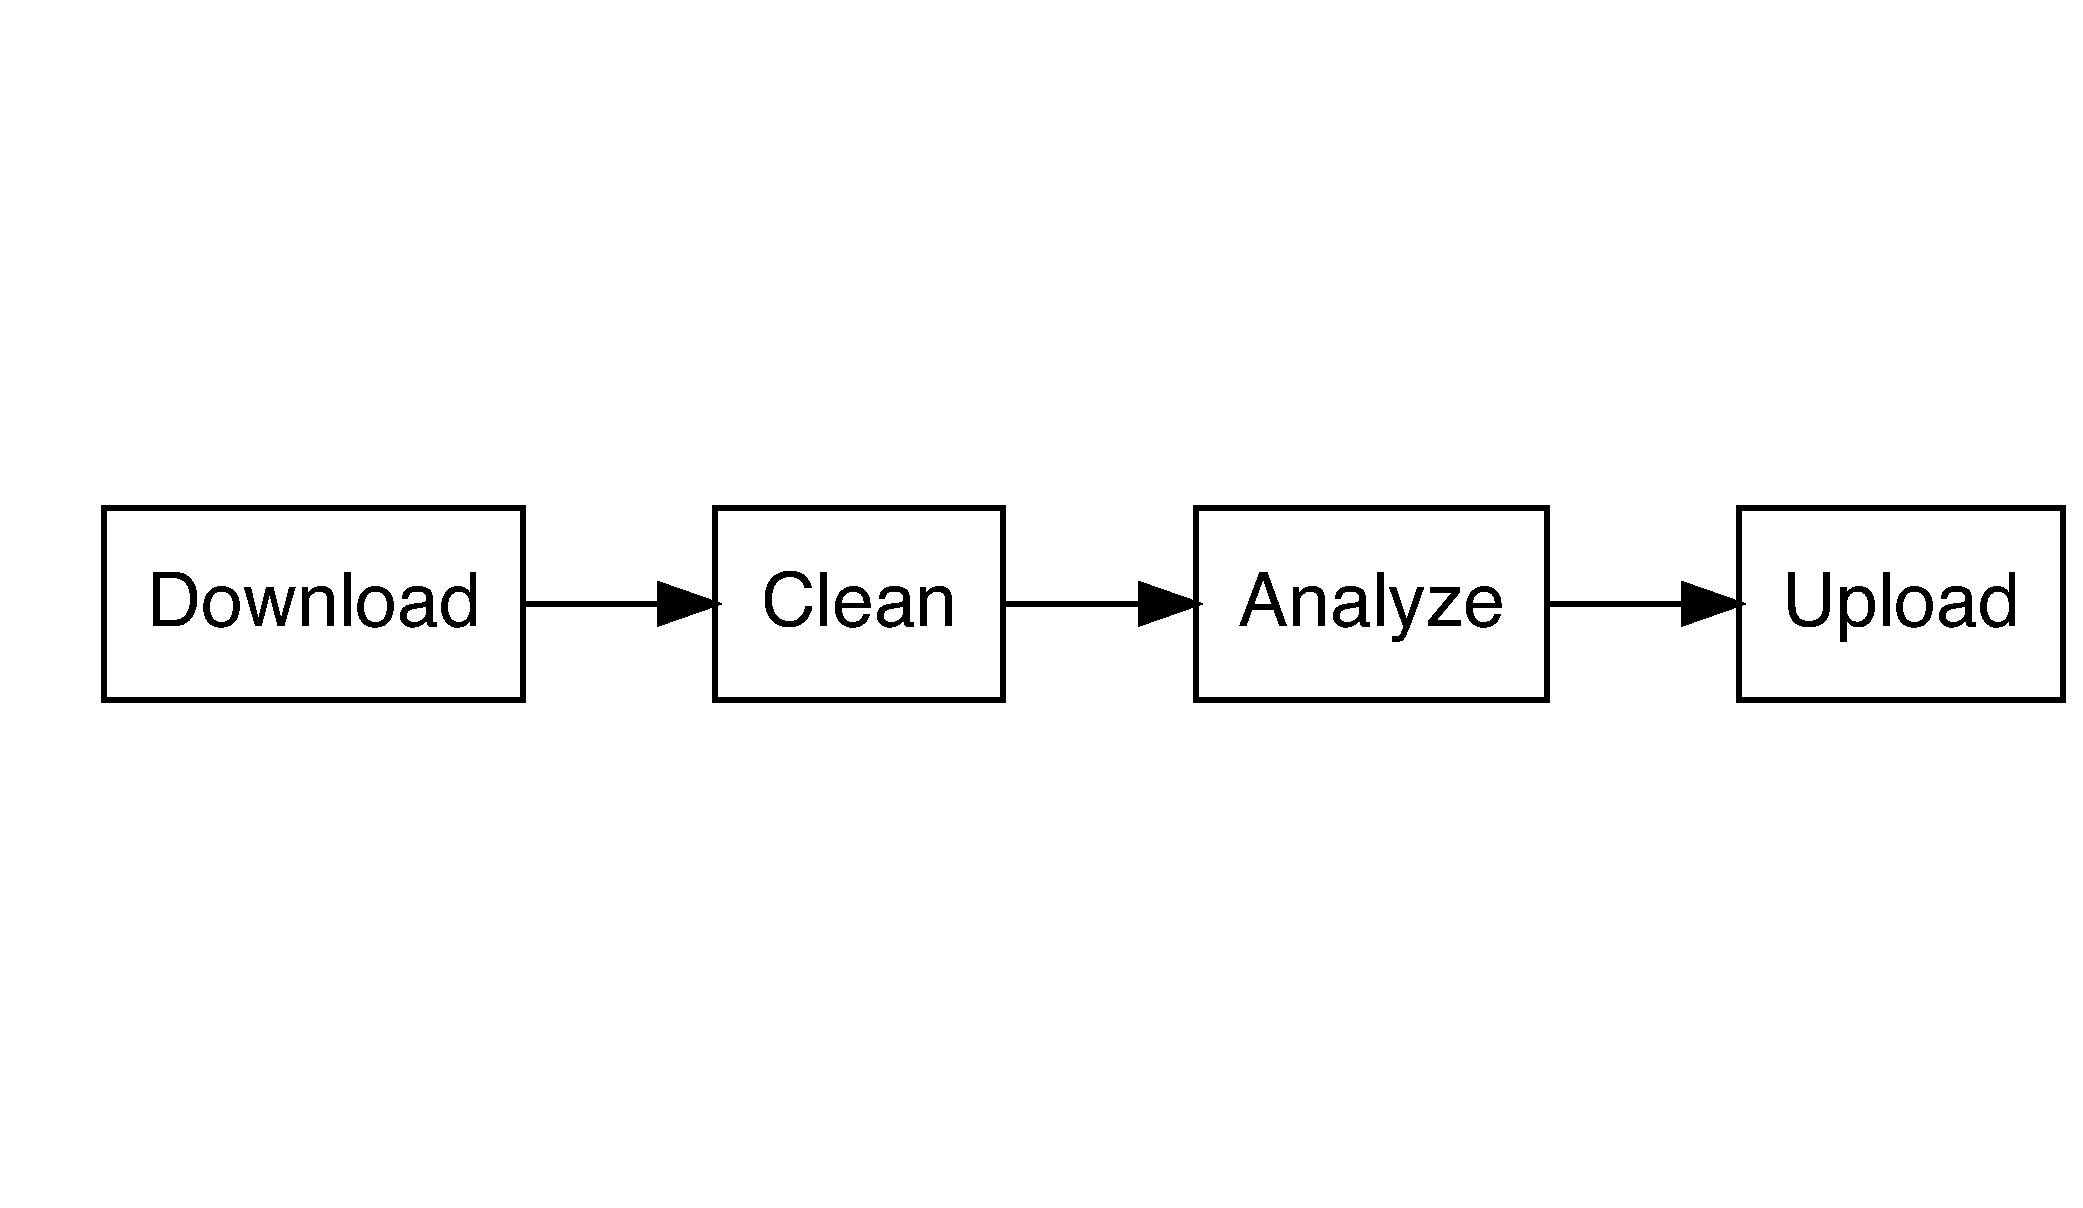
\includegraphics[width=1\linewidth]{Audit_Analytics_with-R_files/figure-latex/unnamed-chunk-181-1}

If you crack open each section, you'll see what you had to perform, which gives you an idea about what functions you may need. For example, you may have downloaded several tables from your accounting software, and a listing of employees from the HR database, amongst the other several procedures you needed to do.

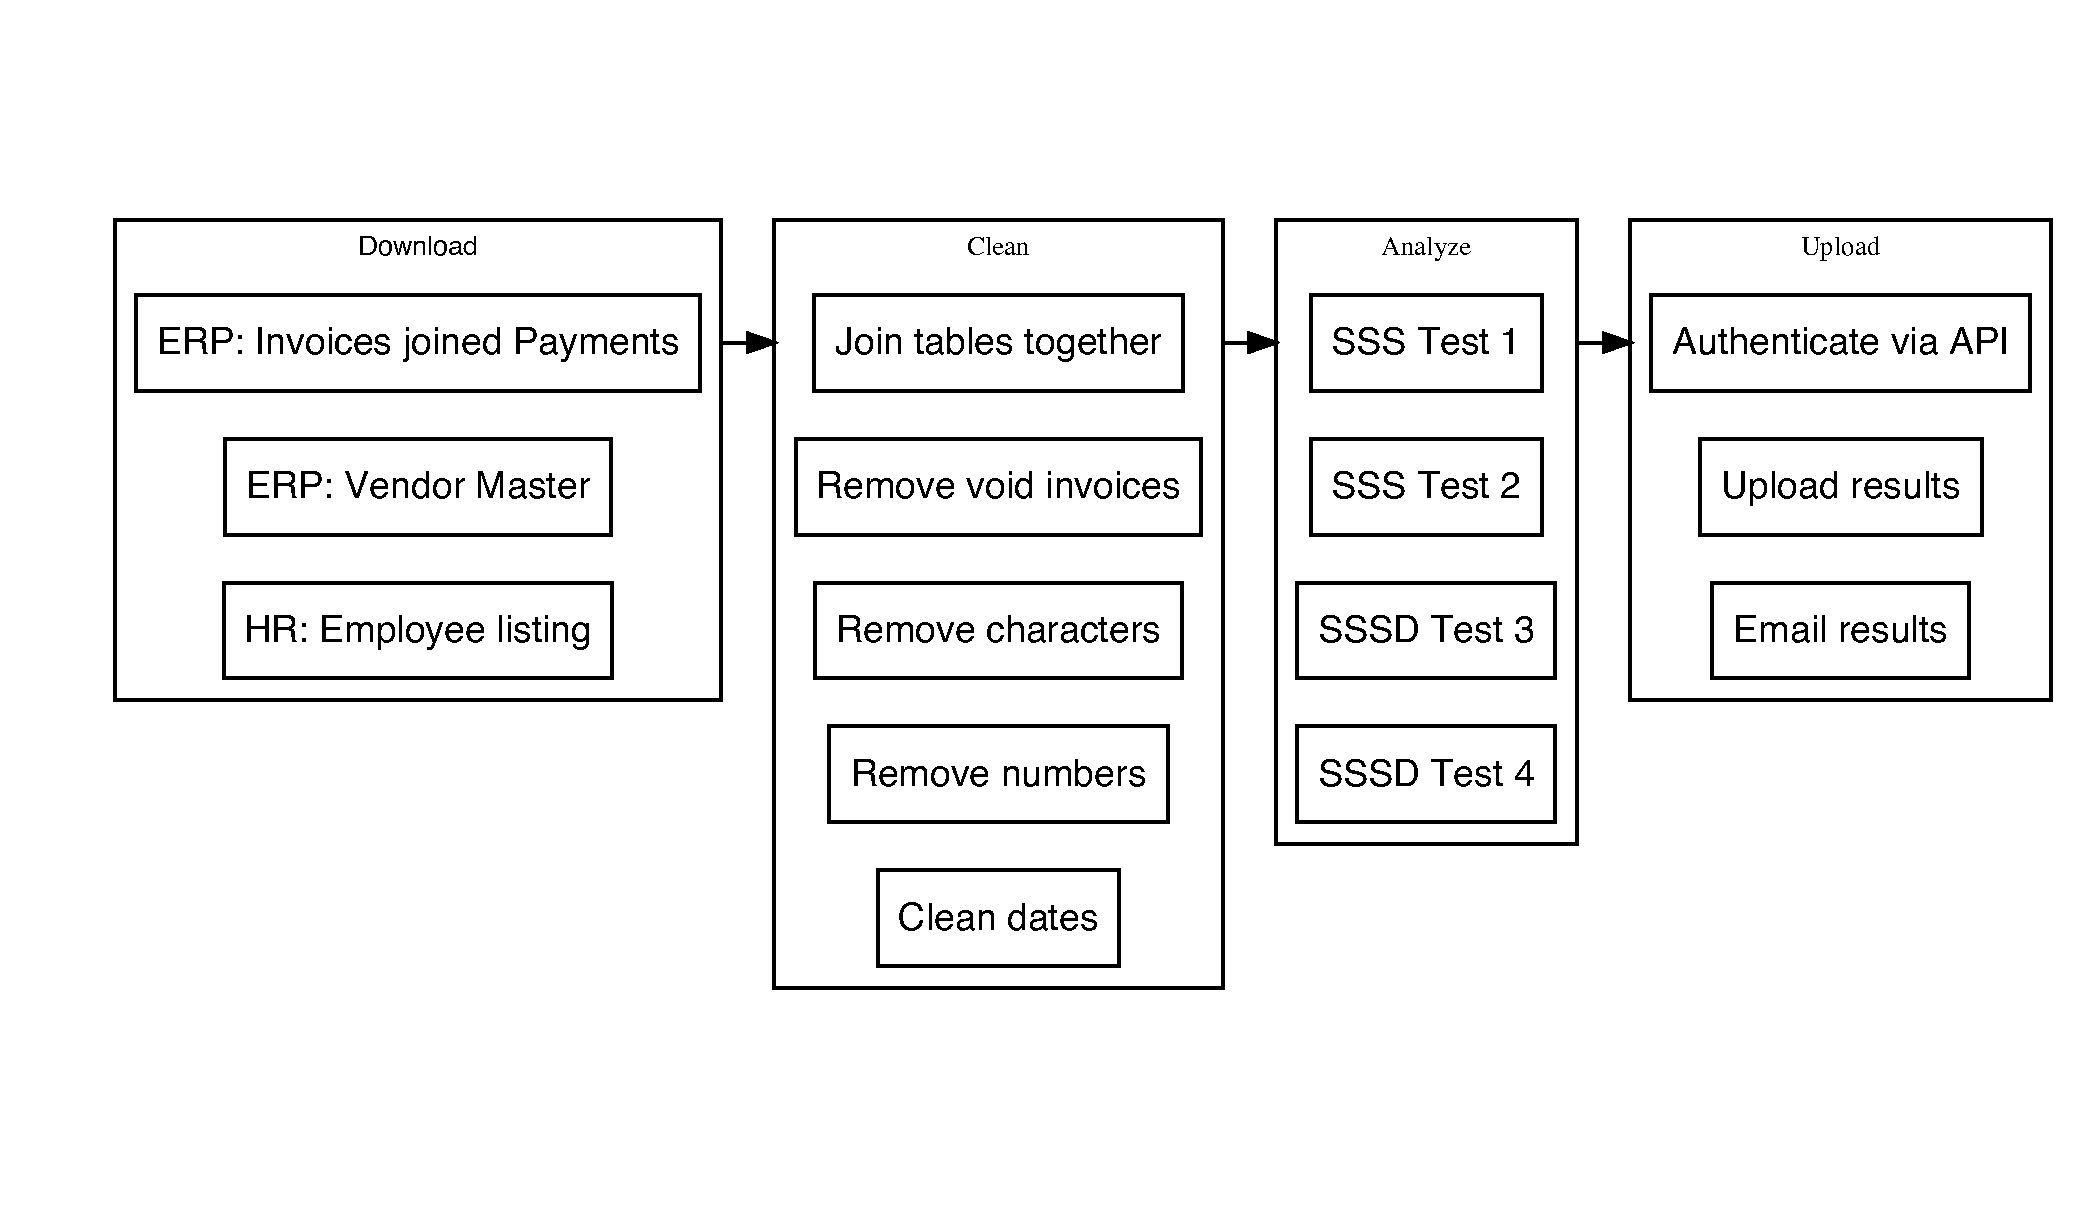
\includegraphics[width=1\linewidth]{Audit_Analytics_with-R_files/figure-latex/unnamed-chunk-182-1}

If you further dig into the download phase, you'll see that you had to create two separate database connections to download information from the ERP and also HR database, before it could be used the even download the information.

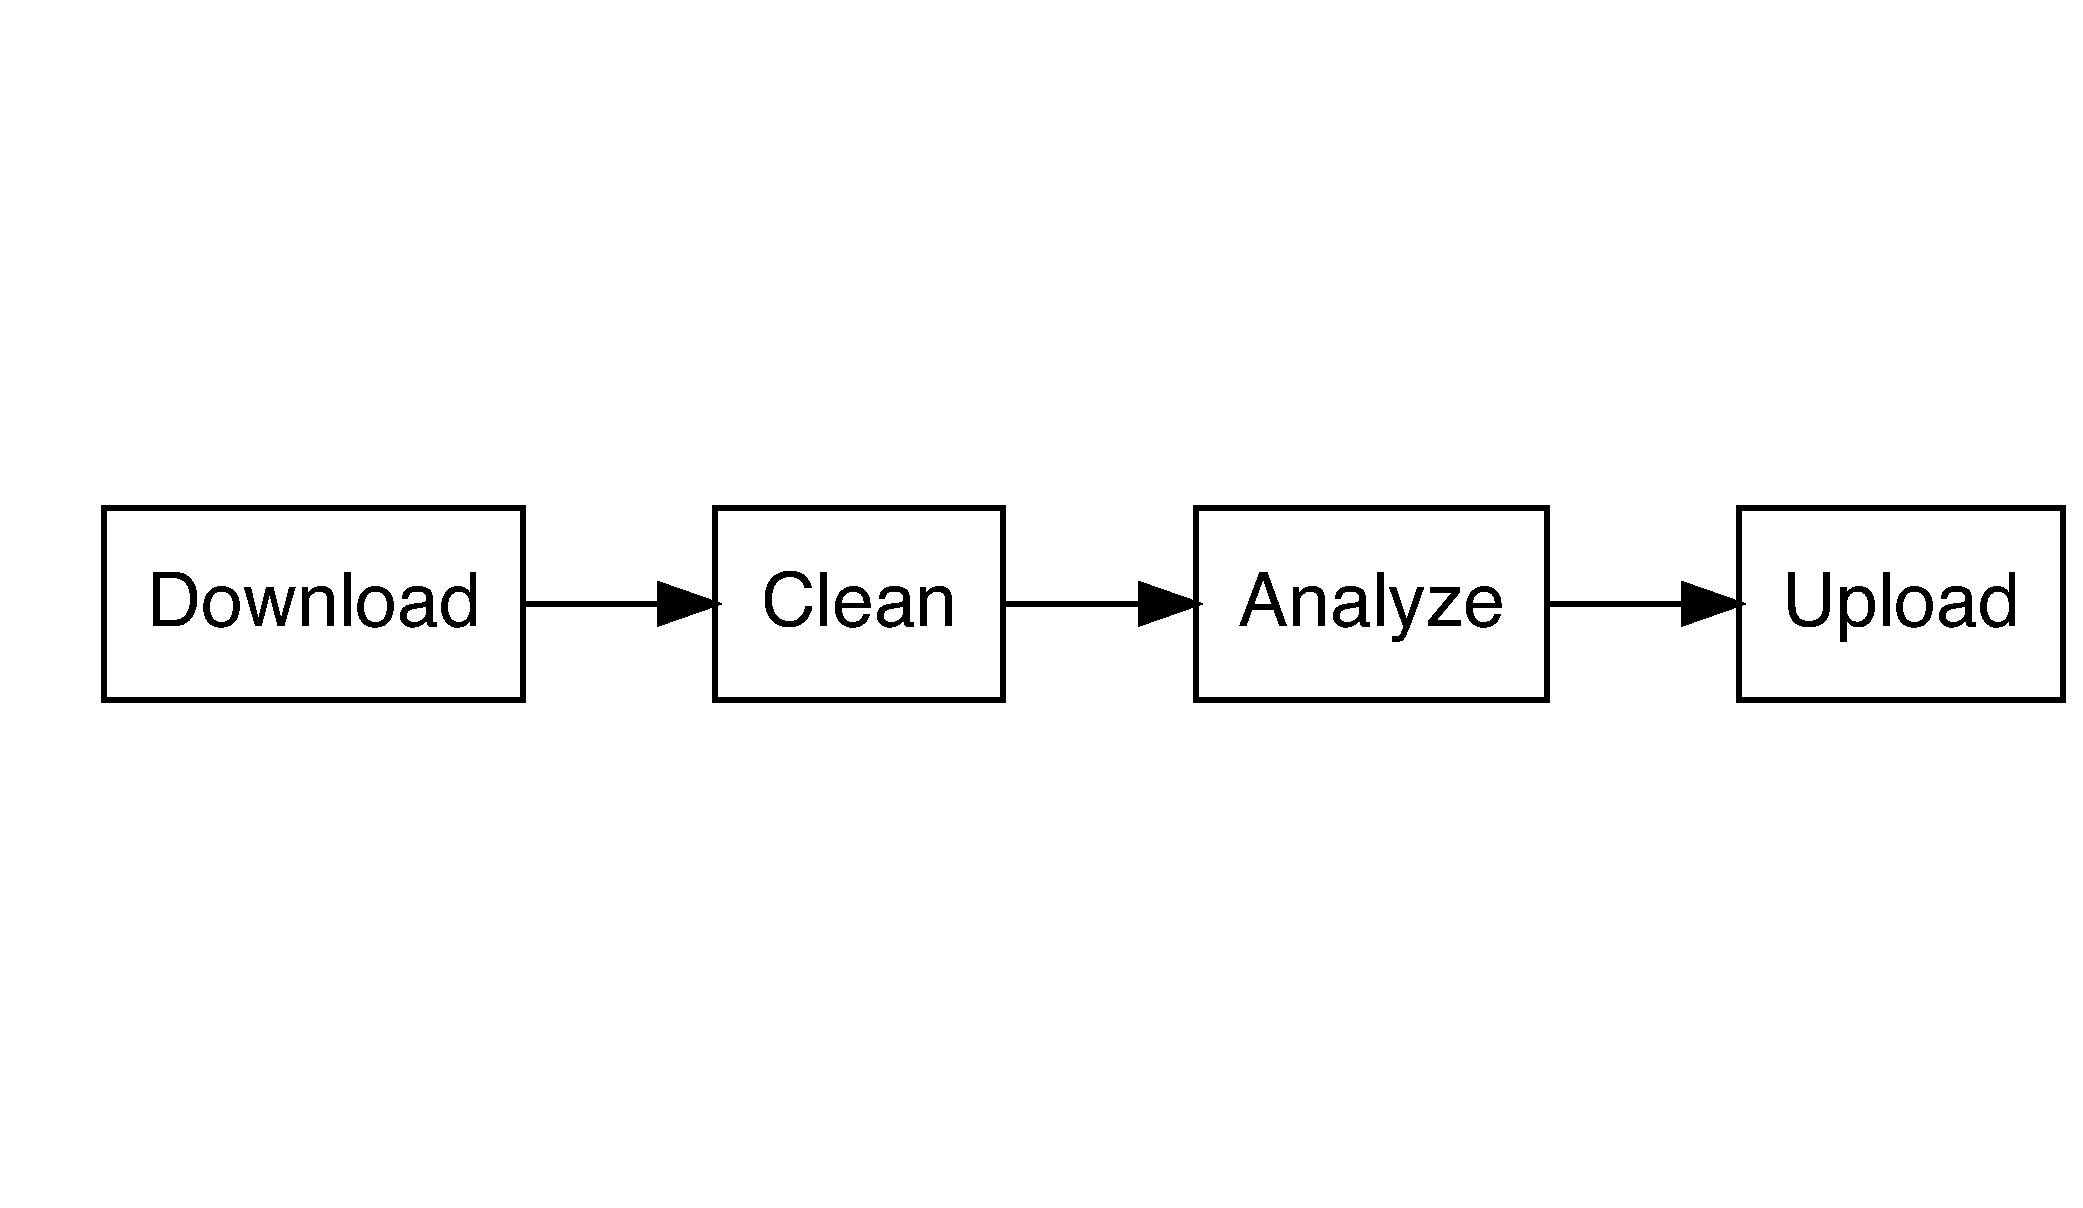
\includegraphics[width=1\linewidth]{Audit_Analytics_with-R_files/figure-latex/unnamed-chunk-183-1}

There are some functions that are worth considering to make. The code you can consider turning into a function could be:

\begin{itemize}
\tightlist
\item
  Database connections to the ERP via Oracle or HR via SQL.
\item
  Downloading and creating of the vendor master, invoices and payments.
\item
  Perform everything - Connecting, downloading and joining the information at the same time.
\end{itemize}

Which ones do you end up choosing to implement? This is a design choice, and is known in programming as cohesion and coupling. \textbf{Cohesion} is where a function does one thing, does it incredibly well, and the inputs and outputs of this are passed between functions. \textbf{Coupling} is how dependent the function is on the input data. Ideally you would choose to retain implement functions that are highly cohesive, and have low coupling.

Database connections, \texttt{connect\_erp()} and \texttt{connect\_hr()}, serve as connectivity mechanisms to their respective databases. These would be reasonably dependent on its input data (a username and password), and would be useful functions to implement. They would quite short and sweet too:

\begin{Shaded}
\begin{Highlighting}[]
\NormalTok{connect_erp <-}\StringTok{ }\ControlFlowTok{function}\NormalTok{(username, password)\{}
\NormalTok{  DBI}\OperatorTok{::}\KeywordTok{dbConnect}\NormalTok{(oracle, }\DataTypeTok{host =}\NormalTok{ erp.abc.com, username, password)}
\NormalTok{\}}
\end{Highlighting}
\end{Shaded}

The \texttt{tbl()} functions serve well for their purpose, which is to point to a specific table. You can further lock in that knowledge by implementing a \texttt{tbl\_erp\_invoices()}, \texttt{tbl\_erp\_payments()} and \texttt{tbl\_hr\_emplist()}. This is still highly cohesive (does one thing: connects to a data table), but also starts to increase coupling (where it is highly dependent on the database connection provided). The increase in coupling may be reasonable - you may choose accept this design and implement these functions, as it is hard to remember exactly the table names that house the data you are looking for.

\begin{Shaded}
\begin{Highlighting}[]
\NormalTok{tbl_erp_invoices <-}\StringTok{ }\ControlFlowTok{function}\NormalTok{(erp)\{}
\NormalTok{  dplyr}\OperatorTok{::}\KeywordTok{tbl}\NormalTok{(erp, }\StringTok{'ap_1200'}\NormalTok{)}
\NormalTok{\}}
\end{Highlighting}
\end{Shaded}

The last option, connecting and downloading all the data you need, may make a monolithic module that is tailored only for one use case, and it also performs too many things. At first glance, this structure seems to make sense because this is how the notebook was written:

\begin{Shaded}
\begin{Highlighting}[]
\NormalTok{all_in_one <-}\StringTok{ }\ControlFlowTok{function}\NormalTok{(username_}\DecValTok{1}\NormalTok{, password_}\DecValTok{1}\NormalTok{, username_}\DecValTok{2}\NormalTok{, password_}\DecValTok{2}\NormalTok{)\{}
\NormalTok{  erp <-}\StringTok{ }\NormalTok{DBI}\OperatorTok{::}\KeywordTok{dbConnect}\NormalTok{(oracle, }\DataTypeTok{host =}\NormalTok{ erp.abc.com, username_}\DecValTok{1}\NormalTok{, password_}\DecValTok{1}\NormalTok{)}
\NormalTok{  sql <-}\StringTok{ }\NormalTok{DBI}\OperatorTok{::}\KeywordTok{dbConnect}\NormalTok{(sql, }\DataTypeTok{host =}\NormalTok{ hr.abc.com, username_}\DecValTok{2}\NormalTok{, password_}\DecValTok{2}\NormalTok{)}
  
\NormalTok{  invoices <-}\StringTok{ }\NormalTok{dplyr}\OperatorTok{::}\KeywordTok{tbl}\NormalTok{(erp, }\StringTok{'ap_1200'}\NormalTok{)}
\NormalTok{  payments <-}\StringTok{ }\NormalTok{dplyr}\OperatorTok{::}\KeywordTok{tbl}\NormalTok{(erp, }\StringTok{'ap_1201'}\NormalTok{)}
\NormalTok{  vendors <-}\StringTok{ }\NormalTok{dplyr}\OperatorTok{::}\KeywordTok{tbl}\NormalTok{(erp, }\StringTok{'vm_5000'}\NormalTok{)}
\NormalTok{  emps <-}\StringTok{ }\NormalTok{dplyr}\OperatorTok{::}\KeywordTok{tbl}\NormalTok{(hr, }\StringTok{'v_emp_list'}\NormalTok{)}
  
\NormalTok{  invoices }\OperatorTok
\StringTok{   }\NormalTok{dplyr}\OperatorTok{::}\KeywordTok{semi_join}\NormalTok{(payments, }\DataTypeTok{by =} \StringTok{'invoice_id'}\NormalTok{)}
\NormalTok{\}}
\end{Highlighting}
\end{Shaded}

However, now we're presented with a function that has low cohesion (its doing multiple things) - it is creating the database connecting, downloading and then joining the tables. Not to mention the two sets of credentials that aren't obviously related to the output:

\begin{itemize}
\tightlist
\item
  The username and password to the ERP database.
\item
  The username and password to the HR database.
\end{itemize}

From a function maintenance perspective, it is difficult to maintain:

\begin{itemize}
\tightlist
\item
  Will you copy and paste the database connections every single time you want to use it elsewhere?
\item
  What happens when this database changes host locations?
\item
  What happens when the ERP is upgraded and the table names change?
\item
  What if you wanted to keep invoices that were both paid and unpaid?
\end{itemize}

While this function technically achieves one highly specific objective, its highly dependent on making sure the company and systems stays constant. With experience, we know this never happens. Given the frailness of the design, a function like this should be used sparingly, and ideally should be kept in a notebook.

\hypertarget{templates}{%
\section{Templates}\label{templates}}

Pre-developed layouts help standardize thought processes and deliverables that your team members should go through when assembling a report. Read more about \href{https://bookdown.org/yihui/rmarkdown-cookbook/package-template.html}{templates within R Markdown}.

Within the \protect\hyperlink{report-structure}{Reporting Section}, we highlight what items are key within an Audit Data Analytics (ADA) notebook. R Markdown templates can be retained within the \texttt{inst/rmarkdown/templates} folder of your package. Specifically, an ADA R Markdown template can be kept at \texttt{inst/rmarkdown/templates/ada/skeletion/skeleton.Rmd}.

\begin{Shaded}
\begin{Highlighting}[]
\NormalTok{---}
\NormalTok{title: "Audit Data Analytics - "}
\NormalTok{author: "Your name"}
\NormalTok{date: "2020-10-29 22:56:30"}
\NormalTok{output:}
\NormalTok{  html_document}
\NormalTok{---}

\FunctionTok{# Objective}

\FunctionTok{# Risks addresses}

\FunctionTok{# Data source}

\FunctionTok{# Data extraction}

\FunctionTok{# Data transformation}

\FunctionTok{# Data completeness}

\FunctionTok{# Test procedures}

\FunctionTok{# Test results}

\FunctionTok{# Session Info}
\BaseNTok{```\{r\}}
\BaseNTok{sessionInfo()}
\BaseNTok{```}
\end{Highlighting}
\end{Shaded}

\hypertarget{continuous-testing}{%
\chapter{Continuous testing}\label{continuous-testing}}

Continuous Monitoring (CM) and Continuous Auditing (CA, or automated controls testing) relies on the same premise - that a specific entity of interest is being evaluated on a high frequency and regular basis. Both definitions are used inconsistently in the audit industry - I tend to rely on CM for general risk measurement, and CA for controls.

Continuous Auditing is a no brainer - who would say no to higher coverage and more tests? Ironically, asking this same question to external auditors can really put them in a bind. Several audit firms do not have explicit guidance on the handling of reliance on internal controls being continuously tested, as current guidance is exclusively pointed towards sampling. See the \protect\hyperlink{appendixct}{appendix} on how to help get started on establishing an agreeable methodology.

\hypertarget{applied-adw}{%
\chapter{Audit Data Mart}\label{applied-adw}}

\hypertarget{other-practices-to-follow}{%
\chapter{Other practices to follow}\label{other-practices-to-follow}}

\hypertarget{documentation}{%
\section{Documentation}\label{documentation}}

As you start, you should promote basic habits instilled into you. Documenting your basic thought process in .R files is generally expected, and the `why' a certain process outlined with comments (lines starting with a \texttt{\#}). The why is important as it explains to code reviewers (external auditors and your peers) the rationale for your approach, or unusual quirks about the data you are transforming.

RMarkdown files become valuable as communication mediums for reports, allowing you to embed a mix of code, graphics, and interactive tables. While most of the exploratory work can be done within a basic .R file, having the ability to readily `knit' a document for sharing increases the people you can share your work with.

Whether you are using R or RMarkdown files, its convenient to have these files as your primary sources of editing as you can use the keyboard shortcuts command-return or control-enter to send a command from the script file to the console.

\hypertarget{passwords}{%
\section{Passwords}\label{passwords}}

TODO Storing secrets - .Renviron, config, keyring

\hypertarget{part-appendix}{%
\part{Appendix}\label{part-appendix}}

\hypertarget{appendixct}{%
\chapter{Continuous testing methodology}\label{appendixct}}

\hypertarget{support-for-continuous-auditing}{%
\section{Support for Continuous Auditing}\label{support-for-continuous-auditing}}

There is a lot of hype around continuous controls testing, and how it will automate or eliminate the need for manual testing or sampling. Regulations have struggled to keep up with the view of continuous testing, despite independent advancements resulting in greater assurances of internal control through these advanced testing mechanisms.

This should not discourage your team in applying analytics on a continuous basis. Rather, it gives you a point to open up conversation with external auditors about how the tests of controls offer greater assurance at a higher degree of efficiency.

\hypertarget{the-requirements-for-evaluting-icfr}{%
\subsection{The requirements for evaluting ICFR}\label{the-requirements-for-evaluting-icfr}}

The Security and Exchange Commission (SEC) provides oversight to the Public Company Accounting Oversight Board (PCAOB), and the PCAOB provides many of the Audit Standards that accounting firms interpret. The SEC explicitly avoids detailing guidance and providing examples to test controls, encouraging companies to design controls to mitigate the risk to the reliability of financial reporting. (``Commission Guidance Regarding Management's Report on Internal Control over Financial Reporting Under Section 13(a) or 15(d) of the Securities Exchange Act of 1934; Final Rule'' \protect\hyperlink{ref-sec-princples-based}{2007})

As a result, if we take a first principles approach, \emph{``The objective of internal control over financial reporting (''ICFR``) is to provide reasonable assurance regarding the reliability of financial reporting and the preparation of financial statements for external purposes in accordance with generally accepted accounting principles (''GAAP``).''} (section A)

Monitoring activities, including \emph{``controls to monitor results of operations and controls to monitor other controls''}, also help address ICFR (A.1.b), and \emph{``For any individual control, different combinations of the nature, timing, and extent of evaluation procedures may provide sufficient evidence.''} (A.2). More specifically, the evidence of the ICFR is allowed to come from on-going monitoring activities (A.2.b), and even to the point where \emph{``evidence from on-going monitoring is sufficient and that no further direct testing is required.''} (A.2.b)

This enables us to critically consider the usage of a strong audit data analytics program in the evaluation of the ICFR. The onus then, is on you to demonstrate high levels of objectivity and competency of the individuals and team for the monitoring program: \emph{``Management's on-going monitoring activities may provide sufficient evidence when the monitoring activities are carried out by individuals with a high degree of objectivity.''} (E.2)

AS 2201 does allow for the use of entity level controls as conducted by internal audit (.24, (``AS 2201: An Audit of Internal Control over Financial Reporting That Is Integrated with an Audit of Financial Statements'' \protect\hyperlink{ref-pcaob-as2201}{2007})) to lower the risk of other controls (.47), and providing sufficient documentation and evidence of operation around the program (.45) may be enough to contribute to the operating effectiveness and evaluation of a control and risk.

\hypertarget{determining-population-tolerable-error-rate}{%
\subsection{Determining population tolerable error rate}\label{determining-population-tolerable-error-rate}}

You should define the methodology you will use to Continuously Audit control operations. The reason to have these conversations with your external auditors is because testing 100\% of the population will invariably find a deviation. It is inevitable, as any control that involves people (or even systems, to an extent) may trip at some point.

One key method to help acknowledge that errors do indeed exist is through clarifying the \emph{population tolerable error rate} - i.e.~the maximum rate of deviations of a prescribed control (.34, (``AS 2315: Audit Sampling'' \protect\hyperlink{ref-pcaob-as2315}{2015})). This will be based upon the control risk that the audit team decides. In addition, when deviations are found, it does not ultimately result in a misstatement either (.35), as there would have to be sufficient evidence proven that all assertions were not met.

Typical sampling asks the auditor to consider control risk, or the \emph{risk of incorrect acceptance} - i.e.~the risk that a control can be deemed effective when it is not. However, when an entire population is considered, this risk effectively reduces to zero, as there is no sampling conducted.

Traditionally, sample sizes are calculated when you know the population tolerable error rate, and the risk of incorrect acceptance. Where \(\beta\) is the risk of incorrect acceptance, \(p_{t}\) is the population tolerable error rate, and \(n\) is the sample size, we can derive the sample size necessary to satisfy audit sampling. (Stewart (\protect\hyperlink{ref-sampling-technical}{2008})) We assume an expectation of no errors in the population with the below:

\[
n = \frac{ln(\beta)}{ln(1 - p_{t})}
\]

In R, if we were to determine the sample size necessary with a risk of incorrect acceptance of 5\% and tolerable error percentage of 5\%, our sample size would be:

\begin{Shaded}
\begin{Highlighting}[]
\NormalTok{b <-}\StringTok{ }\FloatTok{0.05}
\NormalTok{pt <-}\StringTok{ }\FloatTok{0.05}
\KeywordTok{log}\NormalTok{(b) }\OperatorTok{/}\StringTok{ }\KeywordTok{log}\NormalTok{(}\DecValTok{1} \OperatorTok{-}\StringTok{ }\NormalTok{pt)}
\end{Highlighting}
\end{Shaded}

\begin{verbatim}
## [1] 58.40397
\end{verbatim}

If it is difficult to ascertain what the population tolerable error rate may be, it is possible to work backwards from both a \emph{sample size} and an assumption on the control risk. Derived from Sampling Guide technical notes (Stewart (\protect\hyperlink{ref-sampling-technical}{2008})), the population tolerable error rate can be defined as:

\[
p_{t} = -e^\frac{ln(\beta)}{n} + 1
\]
From the previous example, lets say our sample size was 59, and our risk of incorrect acceptance was 10\%, we can estimate the population tolerable error rates.

\begin{Shaded}
\begin{Highlighting}[]
\NormalTok{n <-}\StringTok{ }\DecValTok{59}
\NormalTok{b <-}\StringTok{ }\FloatTok{0.05}
\OperatorTok{-}\KeywordTok{exp}\NormalTok{(}\DecValTok{1}\NormalTok{)}\OperatorTok{^}\NormalTok{(}\KeywordTok{log}\NormalTok{(b) }\OperatorTok{/}\StringTok{ }\NormalTok{n) }\OperatorTok{+}\StringTok{ }\DecValTok{1}
\end{Highlighting}
\end{Shaded}

\begin{verbatim}
## [1] 0.04950761
\end{verbatim}

With this, your methodology could be derived from existing sampling, and you could set your threshold of control operating effectiveness, when tested on the full population, to accept 5\% of samples with errors.

\hypertarget{acl-analytics-to-r}{%
\chapter{ACL Analytics to R}\label{acl-analytics-to-r}}

ACL Analytics is the Audit Command Language and tool, and is useful for analytics teams with novice to expert expertise in analytics. ACL Analytics itself is strongly tied into the Galvanize Highbond cloud software, and development efforts can be done locally prior to uploading into their Robotics tool.

R is useful as your team reaches a higher level of maturity due to its ability to incorporate version control, markdown reports and code packages. The ceiling and technical capabilities required are higher, especially as you move into command prompt oriented software.

Inexperienced teams are encouraged to develop their best audit foundation practices, as it is less about the tool and more about the aptitude. As your team reaches the ceiling of your current toolset and maturity level, then it is worth considering adding to your toolkit.

There are several similarities and differences to help bridge the gap when transferring between the tools, and this appendix will help you bridge the gap.

\hypertarget{import}{%
\section{Import}\label{import}}

\hypertarget{data}{%
\section{Data}\label{data}}

\hypertarget{joins}{%
\subsection{Joins}\label{joins}}

The \href{https://help.highbond.com/helpdocs/analytics/142/scripting-guide/en-us/Content/lang_ref/commands/r_join.htm}{join command} is similar, but there are some syntax and behaviours differences you need to be aware of:

\begin{longtable}[]{@{}lll@{}}
\toprule
\begin{minipage}[b]{0.30\columnwidth}\raggedright
ACL AN\strut
\end{minipage} & \begin{minipage}[b]{0.30\columnwidth}\raggedright
R (tidyverse)\strut
\end{minipage} & \begin{minipage}[b]{0.30\columnwidth}\raggedright
Difference\strut
\end{minipage}\tabularnewline
\midrule
\endhead
\begin{minipage}[t]{0.30\columnwidth}\raggedright
\texttt{JOIN} with no keywords\strut
\end{minipage} & \begin{minipage}[t]{0.30\columnwidth}\raggedright
\texttt{inner\_join(...)}\strut
\end{minipage} & \begin{minipage}[t]{0.30\columnwidth}\raggedright
R will return all matches with all columns in Secondary table, if found in Primary table. \textbf{Can effectively return more rows than exist in Primary table.} AN will return the first match found in the Primary table per row.\strut
\end{minipage}\tabularnewline
\begin{minipage}[t]{0.30\columnwidth}\raggedright
\texttt{PKEY\ \textless{}pkey1\textgreater{}} \texttt{SKEY\ \textless{}skey1\textgreater{}}\strut
\end{minipage} & \begin{minipage}[t]{0.30\columnwidth}\raggedright
\texttt{*\_join(...,\ by\ =\ c(\textquotesingle{}pkey1\textquotesingle{}\ =\ \textquotesingle{}skey1\textquotesingle{},\ \textquotesingle{}pkey2\textquotesingle{}\ =\ \textquotesingle{}skey2\textquotesingle{}))}\strut
\end{minipage} & \begin{minipage}[t]{0.30\columnwidth}\raggedright
Join key goes into the \texttt{by} command. Additional join keys can be added.\strut
\end{minipage}\tabularnewline
\begin{minipage}[t]{0.30\columnwidth}\raggedright
\texttt{FIELDS\ ALL}\strut
\end{minipage} & \begin{minipage}[t]{0.30\columnwidth}\raggedright
\texttt{semi\_join(...)}\strut
\end{minipage} & \begin{minipage}[t]{0.30\columnwidth}\raggedright
Filters the Primary table, only keeping matches that existed in the Secondary table\strut
\end{minipage}\tabularnewline
\begin{minipage}[t]{0.30\columnwidth}\raggedright
\texttt{FIELDS\ \textless{}names\textgreater{}} \texttt{WITH\ \textless{}names\textgreater{}}\strut
\end{minipage} & \begin{minipage}[t]{0.30\columnwidth}\raggedright
\strut
\end{minipage} & \begin{minipage}[t]{0.30\columnwidth}\raggedright
All columns from both tables are kept by design. \texttt{\textless{}names\textgreater{}} of columns can not be specified, and need to be pre-selected beforehand\strut
\end{minipage}\tabularnewline
\begin{minipage}[t]{0.30\columnwidth}\raggedright
\texttt{PRIMARY}\strut
\end{minipage} & \begin{minipage}[t]{0.30\columnwidth}\raggedright
\texttt{left\_join(...)}\strut
\end{minipage} & \begin{minipage}[t]{0.30\columnwidth}\raggedright
Unmatched keys will have secondary column values written as \texttt{NA}\strut
\end{minipage}\tabularnewline
\begin{minipage}[t]{0.30\columnwidth}\raggedright
\texttt{SECONDARY}\strut
\end{minipage} & \begin{minipage}[t]{0.30\columnwidth}\raggedright
\texttt{right\_join(...)}\strut
\end{minipage} & \begin{minipage}[t]{0.30\columnwidth}\raggedright
Unmatched keys will have primary column values be written as \texttt{NA}\strut
\end{minipage}\tabularnewline
\begin{minipage}[t]{0.30\columnwidth}\raggedright
\texttt{PRIMARY\ SECONDARY}\strut
\end{minipage} & \begin{minipage}[t]{0.30\columnwidth}\raggedright
\texttt{full\_join(...)}\strut
\end{minipage} & \begin{minipage}[t]{0.30\columnwidth}\raggedright
Unmatched keys will have primary or secondary column values written as \texttt{NA}\strut
\end{minipage}\tabularnewline
\begin{minipage}[t]{0.30\columnwidth}\raggedright
\texttt{UNMATCHED}\strut
\end{minipage} & \begin{minipage}[t]{0.30\columnwidth}\raggedright
\texttt{anti\_join(...)}\strut
\end{minipage} & \begin{minipage}[t]{0.30\columnwidth}\raggedright
\strut
\end{minipage}\tabularnewline
\bottomrule
\end{longtable}

\hypertarget{analyze}{%
\section{Analyze}\label{analyze}}

\hypertarget{refs}{}
\leavevmode\hypertarget{ref-aicpa2018guide}{}%
AICPA. 2018. \emph{Guide to Data Analytics}. Newark: John Wiley \& Sons, Incorporated.

\leavevmode\hypertarget{ref-pcaob-as2201}{}%
``AS 2201: An Audit of Internal Control over Financial Reporting That Is Integrated with an Audit of Financial Statements.'' 2007. \url{https://pcaobus.org/Standards/Auditing/Pages/AS2201.aspx}.

\leavevmode\hypertarget{ref-pcaob-as2315}{}%
``AS 2315: Audit Sampling.'' 2015. \url{https://pcaobus.org/Standards/Auditing/Pages/AS2315.aspx}.

\leavevmode\hypertarget{ref-sec-princples-based}{}%
``Commission Guidance Regarding Management's Report on Internal Control over Financial Reporting Under Section 13(a) or 15(d) of the Securities Exchange Act of 1934; Final Rule.'' 2007. \url{https://www.sec.gov/rules/interp/2007/33-8810fr.pdf}.

\leavevmode\hypertarget{ref-shop-class}{}%
Crawford, Matthew B. 2009. \emph{Shop Class as Soulcraft: An Inquiry into the Value of Work}.

\leavevmode\hypertarget{ref-rfordatasci}{}%
Hadley Wickham, Garrett Grolemund. 2017. \emph{R for Data Science}. \url{https://r4ds.had.co.nz/index.html}.

\leavevmode\hypertarget{ref-r-pkgs}{}%
Hadley Wickham, Jennifer Bryan. 2020. \emph{R Packages}. \url{https://r-pkgs.org}.

\leavevmode\hypertarget{ref-nigrini-forensicanalytics-ch11}{}%
\emph{Identifying Anomalies Using the Relative Size Factor Test}. 2012. John Wiley \& Sons, Ltd. \url{https://doi.org/10.1002/9781118386798.ch11}.

\leavevmode\hypertarget{ref-nigrini-forensicanalytics-ch12}{}%
\emph{Identifying Fraud Using Abnormal Duplications Within Subsets}. 2012. John Wiley \& Sons, Ltd. \url{https://doi.org/10.1002/9781118386798.ch12}.

\leavevmode\hypertarget{ref-cognitive-ease}{}%
Kahneman, Daniel. 2011. \emph{Thinking, Fast and Slow}.

\leavevmode\hypertarget{ref-outliers}{}%
\emph{NIST/Sematech E-Handbook of Statistical Methods}. n.d. \url{https://www.itl.nist.gov/div898/handbook/prc/section1/prc16.htm}.

\leavevmode\hypertarget{ref-sampling-technical}{}%
Stewart, Trevor R. 2008. ``Technical Notes on the Aicpa Audit Guide Audit Sampling.'' \url{http://cte.univ-setif.dz/coursenligne/cheriguiomar/Ressources/SamplingGuideTechnicalNotes.pdf}.

\leavevmode\hypertarget{ref-tribal-knowledge}{}%
``Tribal Knowledge.'' 2020. \emph{Wikipedia}. Wikimedia Foundation. \url{https://en.wikipedia.org/wiki/Tribal_knowledge}.

\leavevmode\hypertarget{ref-lubridate-help}{}%
Vitalie Spinu, Hadley Wickham, Garrett Grolemund. 2016. \emph{Dates and Times Made Easy with Lubridate}. RStudio. \url{https://lubridate.tidyverse.org/reference/lubridate-package.html}.

\leavevmode\hypertarget{ref-quebec}{}%
``Wikipedia, Name of Quebec City.'' 2020. \emph{Wikipedia}. Wikimedia Foundation. \url{https://en.wikipedia.org/wiki/Name_of_Quebec_City}.

\end{document}
